\chapter{continuità e limiti}
\label{ch:successioni}

\section{funzioni continue}
\label{sec:continuita}

Intuitivamente una funzione continua ha la proprietà
che se in un punto $x_0$ assume un valore $y_0=f(x_0)$ allora
in punti abbastanza vicini ad $x_0$ i valori assunti
non saranno molto diversi dal valore $y_0$.
Nella definizione seguente questo viene formalizzato:
fissato il punto $x_0$ e scelto un errore $\eps>0$
che siamo disposti a commettere sui valori della funzione
possiamo trovare un errore $\delta>0$ per cui nei punti
che differiscono da $x_0$ per meno di $\delta$ il valore
della funzione differisce da $y_0$ per meno di $\eps$.

Se $x$ e $y$ sono due punti di $\RR$ la loro distanza 
è data da $\abs{x-y}$. 
Una disuguaglianza del tipo $\abs{x-y}<r$ significa 
che il punto $x$ si trova nell'intervallo $(x-r,x+r)$.
Nel seguito ci concentreremo sulle funzioni con dominio 
e codominio nei numeri reali. 
Ma potremo osservare che molte delle definizioni e molti 
dei teoremi possono essere enunciati e dimostrati in maniera 
identica anche per le funzioni con dominio e codominio 
nei numeri complessi. 
Ad una prima lettura si consiglia di trascurare 
il caso complesso.
%
\mynote{Ci sono in realtà quattro casi rilevanti:
dominio e codominio reale, dominio e codominio complesso, 
dominio reale e codominio complesso, 
dominio complesso e codominio reale, cominio reale 
e codominio complesso. 
Per dire che il dominio è sottoinsieme dei numeri complessi 
diremo che la funzione $f$ è \emph{di variabile complessa},
mentre per dire che la funzione $f$ ha codominio nei numeri 
complessi diremo che $f$ è \emph{a valori complessi}
o più semplicemente che $f$ è complessa.
Il caso di funzioni complesse di variabile complessa 
è ovviamente il caso più generale. 
Ma a volte può essere utile restringersi alla variabile 
reale dove abbiamo la struttura lineare data dall'ordinamento.
Sempre per mantenere l'ordinamento il caso reale e complesso 
si distinguono anche per i punti all'infinito: nel caso reale 
ne introduciamo due, $+\infty$ e $-\infty$ mentre nel caso 
complesso si introduce un unico punto $\infty$.
}
%
Anche quando $x$ e $y$ sono punti di $\CC$ il modulo della 
differenza $\abs{x-y}$ rappresenta la distanza tra i due 
punti $x$ e $y$. 
Fissato $y\in \CC$ e $r>0$
\mynote{La condizione $r>0$ non ha senso se $r\in \CC$ 
quindi se si impone questa condizione è sottointeso 
che $r\in \RR$}
la condizione $\abs{x-y}<r$ identifica i punti $x$ 
che si trovano all'interno di un cerchio di raggio $r$
intorno a $y$.

\begin{definition}[funzione continua]
  \label{def:continua}%
  \index{funzione!continua}%
  \index{continuità}%
  Sia $f\colon A \subset \RR \to \RR$ 
  (oppure $f\colon A\subset \CC \to \CC$) una funzione. 
  Diremo che $f$ è \emph{continua nel punto}%
\mymargin{continua nel punto}%
\index{continuo!nel punto} $x_0\in A$ se
  \begin{equation}\label{eq:continuita}
  \forall \eps>0 \colon \exists \delta>0 \colon
  \forall x\in A\colon
  \abs{x-x_0} < \delta \implies \abs{f(x)-f(x_0)} < \eps.
  \end{equation}
  
  Diremo che $f$ è \emph{continua}%
\mymargin{continua}%
\index{continuo} se è continua in ogni punto $x_0 \in A$.
  \end{definition}
  
  %%%%%%%%%%%%%%%%%%%
  %%%%%%%%%%%%%%%%%%%
  %%%%%%%%%%%%%%%%%%%
  
  Attenzione: la funzione $f(x)=\frac{1}{x}$
  assume vicino a $x=0$ valori molto diversi tra loro (ad esempio $f(0.01)-f(-0.01)=200$)
  ma ciò non toglie che la funzione possa essere continua in quanto il punto
  $x=0$ non appartiene al dominio e quindi,
  in base alla definizione precedente, non ha senso e non ha importanza
  verificare se la funzione è continua in tale punto.
  
  \begin{theorem}[continuità del reciproco]
  \label{th:cont_reciproco}%
  La funzione $f\colon \RR\setminus\ENCLOSE{0}\to \RR$ definita
  da $f(x)=\frac 1 x$ è una funzione continua.
  \end{theorem}
  %
  \begin{proof}
  Siano $x,x_0\neq 0$.
  Se prendiamo $\delta < \frac{\abs{x_0}}2$
  e se $\abs{x-x_0} < \delta$ si avrà,
  per disuguaglianza triangolare inversa,
  $\abs{x} > \frac{\abs{x_0}}2$. Dunque
  \[
  \abs{\frac 1 x - \frac 1 {x_0}}
  = \frac{\abs{x-x_0}}{\abs{x\cdot x_0}}
  \le \frac{2\delta}{\abs{x_0}^2}.
  \]
  Si ottiene quindi la condizione $\abs{f(x)-f(x_0)}<\eps$
  se si sceglie $\delta$ in modo che
  risulti anche $\delta < \frac{\abs{x_0}^2\cdot \eps}{2}$.
  \end{proof}
  
  \begin{example}
  La \emph{funzione segno}%
\mymargin{funzione segno}%
\index{funzione!segno} $\sgn\colon \RR \to \RR$ definita da
  \[
    \sgn(x) = \begin{cases}
    1 & \text{se $x> 0$}\\
    0 & \text{se $x=0$}\\
    -1 & \text{se $x<0$}
    \end{cases}
  \]
  è un esempio di funzione non continua.
  \end{example}
  %
  \begin{proof}
  Verifichiamo che la funzione non è continua
  nel punto $x_0=0$.
  Infatti se $x\neq 0$ si ha
  \[
  \abs{\sgn(x)-\sgn(x_0)} = \abs{\sgn(x)} = 1
  \]
  e quindi se scegliamo $\eps<1$ non è possibile
  trovare $\delta>0$ per cui valga la condizione
  di continuità~\eqref{eq:continuita}
  nel punto $x_0=0$.
  \end{proof}
  
  \begin{exercise}
  Dimostrare che le funzioni $f(x) = x$ e $g(x)=\abs{x}$ sono continue.
  Dimostrare che le funzioni $h(x) = \lfloor x\rfloor$ e $k(x)=\lceil x \rceil$
  non sono continue (ma sono continue in ogni punto
  $x_0\in \RR \setminus \ZZ$).
  \end{exercise}
  
  \begin{definition}[operazioni sulle funzioni]
  Sia $A \subset \RR$ (oppure $A\subset \CC$) 
  e siano $f,g$ funzioni $A \to \RR$ (oppure $A\to \CC$).
  Possiamo allora definire
  $f+g$, $-f$, $f-g$, $f\cdot g$, $\abs f$, $f^n$ (con $n\in \NN$)
  e (se $g(x)\neq 0$ per ogni $x\in A$) anche $f/g$
  come funzioni $A \to \RR$ (o $A\to \CC$) mediante le seguenti ovvie
  definizioni
  \begin{gather*}
  (f+g)(x) = f(x) + g(x), \qquad
  (f-g)(x) = f(x) - g(x), \\
  (f\cdot g)(x) = f(x) \cdot g(x), \qquad
  (f/g)(x) = f(x) / g(x), \\
  (-f)(x) = -(f(x)), \qquad
  \abs f(x) = \abs{f(x)}, \qquad
  f^n(x) = (f(x))^n.
  \end{gather*}
  
  Se $f\colon A \to B$ e $g\colon B\to C$ ricordiamo
  che abbiamo definito la funzione composta
  $g\circ f\colon A \to C$:
  \[
    (g\circ f)(x) = g(f(x)).
  \]
  
  Se $c\in \RR$ (o $c\in \CC$) è un numero considereremo a volte 
  $c\colon A \to \RR$ come una funzione \emph{costante}.
  Risulta quindi inteso che $c\cdot f$ è la funzione definita da
  $(c\cdot f)(x) = c\cdot (f(x))$.
  La somma e il prodotto per costante rendono l'insieme $\RR^A$
  delle funzioni $A \to \RR$ uno spazio vettoriale sul campo $\RR$
  (lo stesso vale per $\CC^A$ con $A\subset \CC$)
  \end{definition}
  
  \begin{theorem}[composizione di funzioni continue]
  \label{th:continuita_composizione}%
  Se $f$ e $g$ sono funzioni (reali o complesse) definite e continue
  in uno stesso punto $x_0$ (reale o complesso)
  allora anche
  \[
    f+g, \qquad
    f\cdot g, \qquad
    f-g, \qquad
    \abs{f}, \qquad
    f^n\ \text{(con $n\in \NN$)}
  \]
  sono funzioni definite e continue nel punto $x_0$.
  Se inoltre $g(x_0)\neq 0$ anche la funzione
  $f/g$
  è definita e continua nel punto $x_0$.
  
  Se $f\colon A\subset \RR \to \RR$ è una funzione continua
  nel punto $x_0\in A$ e
  $g\colon B\subset \RR \to \RR$ è una funzione
  continua nel punto $y_0=f(x_0)\in B$ allora la funzione $g\circ f$
  definita in $f^{-1}(B)$ è continua nel punto $x_0$
  (lo stesso vale sostituendo $\CC$ ad $\RR$)
  \end{theorem}
  %
  \begin{proof}
  Mostriamo prima di tutto la continuità
  della composizione $g\circ f$.
  Per la continuità di $f$ in $x_0$ e di $g$ in $y_0=f(x_0)$
  si ha che per ogni $\eps>0$ esiste un $\gamma>0$
  e per ogni $\gamma>0$ esiste un $\delta>0$ per cui
  \begin{align*}
   \abs{x-x_0}< \delta &\implies \abs{f(x)-f(x_0)}<\gamma,\\
   \abs{y-y_0}< \gamma & \implies \abs{g(y)-g(y_0)}<\eps
  \end{align*}
  da cui
  \[
  \abs{x-x_0}< \delta
  \implies \abs{f(x)-f(x_0)}< \gamma
  \implies \abs{g(f(x))-g(f(x_0))} < \eps
  \]
  che non è altro che la condizione di
  continuità~\eqref{eq:continuita} per $g\circ f$.
  
  Se $f$ e $g$ sono continue nel punto $x_0$
  allora per ogni $\eps'>0$ esistono $\delta_1$
  e $\delta_2$ tali che
  \begin{align*}
   \abs{x-x_0} < \delta_1 &\implies \abs{f(x)-f(x_0)} < \eps',
   \\
   \abs{x-x_0} < \delta_2 &\implies \abs{g(x)-g(x_0)} < \eps'.
  \end{align*}
  In particolare scegliendo $\delta = \min\ENCLOSE{\delta_1,\delta_2}$
  se $\abs{x-x_0} < \delta$ valgono contemporaneamente
  entrambe le stime:
  \[
   \abs{f(x)-f(x_0)}< \eps', \qquad
   \abs{g(x)-g(x_0)}< \eps'.
  \]
  
  Dunque per la somma osserviamo che se $\abs{x-x_0}<\delta$
  si ha
  \begin{align*}
   \abs{(f+g)(x) - (f+g)(x_0)}
    &= \abs{f(x)+g(x)-f(x_0)-g(x_0)}\\
    &\le \abs{f(x)-f(x_0)} + \abs{g(x)-g(x_0)}
    \le 2 \eps'.
  \end{align*}
  Dato $\eps>0$ basterà quindi scegliere $\eps' = \eps / 2$
  e $\delta$ come sopra per ottenere la condizione di continuità.
  
  Per il prodotto si ha
  \begin{align*}
    \MoveEqLeft \abs{f(x)g(x)-f(x_0)g(x_0)}\\
    &= \abs{f(x)g(x) - f(x_0)g(x) + f(x_0)g(x) - f(x_0)g(x_0)}\\
    &\le \abs{f(x)-f(x_0)}\cdot\abs{g(x)} + \abs{f(x_0)}\cdot \abs{g(x)-g(x_0)} \\
    &\le \eps' \abs{g(x)} + \abs{f(x_0)} \eps'.
  \end{align*}
  Osserviamo ora che $\abs{g(x)}\le \abs{g(x)-g(x_0)} + \abs{g(x_0)}$
  e quindi $\abs{g(x)}\le \abs{g(x_0)}+\eps'$ da cui:
  \begin{align*}
    \abs{f(x)g(x)-f(x_0)g(x_0)}
    &\le \eps' \enclose{\abs{g(x_0)}+\eps'} + \abs{f(x_0)} \eps' \\
    &= \eps' \cdot(\abs{f(x_0)} + \abs{g(x_0)} + \eps').
  \end{align*}
  Possiamo facilmente rendere questa quantità inferiore a
  qualunque $\eps>0$: basterà prendere $\eps'<1$ e
  \[
    \eps' < \frac{\eps}{\abs{f(x_0)} + \abs{g(x_0)} + 1}.
  \]
  
  La funzione $f^n$ è continua per induzione su $n$
  in quanto prodotto di funzioni
  continue: $f^{n+1} = f^{n} \cdot f$.
  
  Abbiamo già visto che la funzione $h(x) = \frac{1}{x}$ è continua,
  dunque se $g$ è continua anche la funzione $\frac{1}{g(x)} = h\circ g$
  è continua essendo composizione di funzioni continue. 
  Di conseguenza anche la funzione $\frac{f}{g} = f \cdot \frac{1}{g}$
  è continua, essendo il prodotto di funzioni continue.
  
  Analogamente la funzione $f-g$ è la somma di $f$ con $-g$ e
  la funzione $-g$ è la composizione di $g$ con $h(x)=-x$.
  E' immediato verificare che la funzione $h(x)=-x$ è continua
  e dunque anche la differenza $f-g$ è continua.
  Lo stesso vale per la funzione $\abs f$ che è la composizione
  di $f$ con la funzione $h(x) = \abs{x}$.
  \end{proof}
  
  Il precedente teorema è molto importante ed utile in quanto
  garantisce che ogni funzione definita tramite una espressione
  che coinvolge solamente le funzioni e le operazioni
  elencate nell'enunciato del teorema, risulta certamente
  essere una funzione continua. Come nel seguente.
  
  \begin{example}
  La funzione
  \[
  f(x) = \frac{(x-3)\cdot x -\frac{1}{x+x^2}}{\abs{x-\frac{1-x^3}{x}}}
  \]
  è continua.
  
  Si intende che tale funzione è definita sull'insieme degli $x\in \RR$
  per cui tutte le operazioni coinvolte sono definite ovvero
  $f\colon D \subset \RR \to \RR$
  con
  \[
    D = \ENCLOSE{x\in \RR \colon x+x^2 \neq 0,\ x\neq 0,\ \abs{x-\frac{1-x^3}{x}}\neq 0}.
  \]
  \end{example}
  \begin{proof}
  Per convincersi che questa funzione $f$ è continua
  si nota che le funzioni $x$ e le costanti $3$ e $1$ sono
  funzioni continue.
  Ma allora, per il teorema~\ref{th:continuita_composizione},
  anche le funzioni $x-3$ e $x^2=x\cdot x$ sono continue.
  Dunque anche $(x-3)\cdot x$, $x+x^2$ e $x^3$ e $1-x^3$ sono continue.
  Di conseguenza sono continue pure $\frac 1{1+x^2}$ e $\frac{1-x^3}{x}$.
  E poi saranno continue anche $(x-3)\cdot x - \frac 1{1+x^2}$ e $x-\frac{1-x^3}{x}$
  e quindi $x-\frac{1-x^3}{x}$ e pure $\abs{x-\frac{1-x^3}{x}}$. Infine sarà
  dunque continua $f(x)$.
  \end{proof}
  
  In particolare è chiaro che le funzioni lineari e quadratiche 
  che abbiamo introdotto nelle sezioni precedenti sono funzioni continue
  in quanto sono ottenute sommando e moltiplicando tra loro funzioni continue.
  
  %%%%%%%%%%%%%%%%%%%
  
  \begin{theorem}[continuità delle funzioni monotone]
    \label{th:monotona_continua}%
    \mymark{*}%
    \index{funzione!continua}%
    \index{funzione!monotòna}%
    \index{funzione!suriettiva}%
    Sia $A\subset \RR$ e sia
    $f\colon I \to \RR$ una funzione monotòna.
    Se $f(I)$ è un intervallo allora $f$ è continua.
%    \label{th:monotona_continua_reverse}%
%    Allora $f$ è continua se e solo se $f(I)$ è 
%    un intervallo.
\end{theorem}
  %
  \begin{proof}
  Senza perdita di generalità possiamo supporre che $f$ 
  sia crescente. 
  % Dimostriamo innanzitutto che se $f(I)$ è intervallo allora $f$ è continua.
  
  Prendiamo un punto $x_0\in I$ e sia $\eps>0$.
  Vogliamo trovare $x_1<x_0$ tale che  
  per ogni $x\in [x_1,x_0]\cap I$ si abbia $f(x)>f(x_0)-\eps$.
  Siccome $f(I)$ è un intervallo che contiene il punto $f(x_0)$ 
  ci sono due possibilità: o $f(x)>f(x_0)-\eps$ per ogni $x\in I$
  e quindi possiamo scegliere $x_1<x_0$ a piacere
  oppure esiste $x_1\in I$ tale che $f(x_1)=f(x_0) - \frac \eps 2$.
  In questo secondo caso dovrà essere $x_1<x_0$ (in quanto $f$ è crescente)
  e per monotonia si avrà, come voluto $f(x)\ge f(x_1) > f(x_0)-\eps$ 
  per ogni $x\in [x_1,x_0]$.
  
  In modo analogo possiamo trovare $x_2>x_0$ tale 
  che per ogni $x\in [x_0,x_2]\cap I$ si abbia $f(x) < f(x_0)+\eps$.
  Essendo $f$ crescente se $x\ge x_0$ si avrà anche $f(x)\ge f(x_0)$ 
  e se $x\le x_0$ si avrà $f(x) \le f(x_0)$. 
  Dunque per ogni $x\in [x_1,x_2]$ si avrà $\abs{f(x)-f(x_0)}<\eps$.
  Basterà scegliere $\delta = \min\ENCLOSE{x_0-x_1,x_2-x_0}$ 
  per ottenere la continuità di $f$ in $x_0$.
  
%  Supponiamo ora che $f$ sia una funzione continua e crescente.
%  Vogliamo dimostrare che $f(I)$ è un intervallo.
%  
%  Siano $y_1, y_2 \in f(I)$ e sia $y_0\in \RR$
%  con $y_1 < y_0 < y_2$.
%  Vogliamo dimostrare che $y_0\in f(I)$ cioè che esiste $x_0\in I$
%  tale che $f(x_0)=y_0$.
%  Sappiamo che esistono $x_1,x_2$ in $I$ tali che
%  $f(x_1) = y_1$ e $f(x_2) = y_2$.
%  Dovrà essere $x_1<x_2$ perché $f(x_1)<f(x_2)$ e
%  $f$ è crescente.
%  Definiamo:
%  \[
%   x_0 = \sup A
%  \qquad
%  \text{con } A=\ENCLOSE{x\in I\colon f(x)<y_0},
%  \]
%  e dimostriamo che $f(x_0)=y_0$. 
%  Chiaramente $x_0\in [x_1,x_2]$ in quanto 
%  $x_1\in A$ e $x_2$ è un maggiorante di $A$
%  e dunque $f$ è definita e continua in $x_0$.
%  
%  Se fosse $f(x_0)<y_0$ scelto $\eps = y_0-f(x_0)$
%  per la definizione di continuità dovrebbe esistere
%  $\delta>0$ tale che per ogni $x\in I$ con $\abs{x-x_0}<\delta$
%  si abbia $\abs{f(x)-f(x_0)}<\eps$.
%  In particolare scelto $x=x_0+\frac \delta 2$
%  si avrebbe $f(x) < f(x_0) + \eps = y_0$.
%  Ma allora avremmo $x\in A$ che è assurdo in quanto
%  $\sup A = x_0 < x$.
%  
%  Se fosse invece $f(x_0)>y_0$ posto $\eps = f(x_0)-y_0$,
%  grazie alla continuità di $f$ in $x_0$,
%  possiamo trovare $\delta>0$ tale che per ogni $x\in I$
%  con $\abs{x-x_0}<\delta$ si abbia $\abs{f(x)-f(x_0)}<\eps$.
%  In particolare scelto $t = x_0 - \frac \delta 2$
%  si ha $f(t) > f(x_0)-\eps = y_0$. 
%  Ma essendo $t<x_0 = \sup A$ sappiamo che $t$ non può essere 
%  un maggiorante di $A$ dunque deve esistere $x\in A$
%  tale che $t<x$. 
%  Ma se $x\in A$ allora $f(x) < y_0 < f(t)$
%  che è assurdo in quanto $f$ è crescente.
%  
%  Abbiamo quindi mostrato che $f(x_0)=y_0$. 
%  Questo è vero per ogni scelta di $y_1<y_2$ in $f(I)$
%  dunque $f(I)$ è un intervallo.
\end{proof}
  %

Il teorema precedente (teorema~\ref{th:monotona_continua}) 
ci permette di affermare che per $a>0$, $a\neq 1$ 
le funzioni $\exp_a$ e $\log_a$ sono continue. 
Infatti tali funzioni sono bigezioni monotone tra 
gli intervalli $\RR$ e $\RR_+$.

Anche le funzioni trigonometriche $\sin$ e $\cos$ sono funzioni continue.
Sappiamo infatti che $\sin \colon [-\tau/4,\tau /4]\to [-1,1]$
e $\cos\colon [0,\tau/2]\to [-1,1]$ sono strettamente monotone 
e bigettive dunque sono continue su tali intervalli. 
Grazie alle proprietà di simmetria e periodicità
(oppure utilizzando le formule di addizione) è facile verificare 
che tali funzioni sono continue su tutto $\RR$.

Grazie al teorema~\ref{th:continuita_composizione} sappiamo 
che se $n\in \NN$ la funzione $x^n$ è continua su tutto il suo 
dominio $\RR$. 
La funzione inversa $\sqrt[n]{x}$ è anch'essa crescente e 
bigettiva come funzione $[0,+\infty)\to[0,+\infty)$ e dunque 
anch'essa risulta essere continua.
Per simmetria (si veda l'esercizio~\ref{ex:simmetrica_continua}) 
possiamo concludere 
%che sia la potenza $x^n$ 
che le radici $\sqrt[n]{x}$ sono 
funzioni continue su tutto il loro dominio.
Anche la funzione $f(x) = x^\alpha$, $f\colon [0,+\infty)\to [0,+\infty]$ 
con $\alpha>0$ è crescente ed è invertibile (l'inversa è $x^{\frac 1 \alpha}$)
e dunque è surgettiva e continua.
Se $\alpha<0$ la funzione $f(x)=x^\alpha$ è definita sull'intervallo 
$(0,+\infty)$ ed è anch'essa continua in quanto 
composizione di funzioni continue: $x^{\alpha} = \frac{1}{x^{-\alpha}}$.

%
\begin{exercise}\label{ex:simmetrica_continua}
  Sia $f\colon \RR\to \RR$ una funzione pari oppure dispari.
  Se la restrizione di $f$ all'intervallo $[0,+\infty)$ 
  è continua allora $f$ è continua su tutto $\RR$.
\end{exercise}

\subsection{limite}

Se una funzione $f$ non è definita in un punto $x_0$ non ha senso chiedersi
se in tale punto è continua. 
Possiamo però chiederci se è possibile definire la funzione anche nel punto 
$x_0$ dando un valore opportuno $\ell$ in modo da rendere $f$ continua 
in quel punto. 
Se ciò è possibile diremo che la funzione $f(x)$ ha limite $\ell$ 
per $x$ che tende a $x_0$ e scriveremo:
\[
  f(x) \to \ell \qquad \text{per $x\to x_0$}
\]
(daremo tra poco una definizione con maggiore precisione e generalità).

Ad esempio la funzione $f(x) = \frac{x^2-1}{x-1}$ è una funzione definita per $x\neq 1$
e coincide, se $x\neq 1$ con la funzione lineare $\tilde f(x) = x+1$ definita 
su tutto $\RR$. 
Visto che $\tilde f$ è continua e $\tilde f(1)=2$
scriveremo:
\[
  \frac{x^2-1}{x-1} \to 2
  \qquad \text{per $x\to 1$.}
\]

Se estendiamo $f$ con un valore $\ell$ nel punto $x_0$ otteniamo 
in generale la funzione 
\[
  \tilde f(x) = \begin{cases}
    f(x) & \text{se $x\neq x_0$}\\
    \ell & \text{se $x=x_0$}
  \end{cases}  
\]
e la continuità di $\tilde f$ nel punto $x_0$ si scrive così:
\[
\forall\eps>0\colon \exists \delta>0\colon
\abs{x-x_0}<\delta \implies \abs{\tilde f(x)-\tilde f(x_0)}<\eps.  
\]
Osserviamo che se $x=x_0$ allora ovviamente $\abs{\tilde f(x)-\tilde f(x_0)}
= 0 < \eps$ dunque possiamo supporre, nella condizione precedente, 
che sia $x\neq x_0$ e dunque $\tilde f(x)=f(x)$. 
Inoltre visto che $\tilde f(x_0)=\ell$ 
e $\tilde f(x)=f(x)$ se $x\neq x_0$,
si ottiene 
la seguente condizione:
\begin{equation}\label{eq:55338}
\forall \eps>0\colon \exists \delta >0 \colon 
  \forall x\neq x_0\colon
  \abs{x-x_0}<\delta \implies \abs{f(x) - \ell} < \eps.
\end{equation}
La~\eqref{eq:55338} potrebbe dunque essere utilizzata per definire 
il concetto di limite $f(x)\to \ell$ per $x\to x_0$.
Sarà però molto utile estendere il concetto di limite $f(x)\to \ell$ 
per $x\to x_0$ anche nei casi in cui $\ell$ e/o $x_0$ possano 
essere infiniti (cioè elementi dei reali estesi $\bar \RR$).

Per fare ciò osserviamo che
se definiamo%
\mynote{%
la lettera $B$ sta per \emph{ball} in quanto 
più in generale (se fossimo in $\RR^3$ invece che in $\RR$)
l'insieme dei punti che distano meno di $\rho$ da un punto fissato 
è l'interno di una sfera piena. 
In geometria una sfera piena si chiama \emph{palla} 
se contiene solo i punti interni (e non la superficie sferica)
e si chiama \emph{disco} o \emph{palla chiusa} se contiene 
anche i punti della superficie.
}
$B_\rho(x_0) = \ENCLOSE{x\in \RR \colon \abs{x-x_0}<\rho}$
la condizione \eqref{eq:55338}
può essere scritta anche nella forma 
\[
  \forall \eps>0\colon \exists \delta >0 \colon 
  x \in B_\delta(x_0)\setminus\ENCLOSE{x_0} \implies f(x) \in B_\eps(\ell)  
\]
che a sua volta si può scrivere nella forma:
\[
  \forall \eps>0\colon \exists \delta >0 \colon 
  f(B_\delta(x_0)\setminus\ENCLOSE{x_0}) \subset  B_\eps(\ell).    
\]

L'idea è che gli insiemi del tipo
$B_\rho(x_0)$ 
rappresentano i punti \emph{vicini} al punto $x_0$. 
In analogia potremmo pensare che i punti \emph{vicini} 
a $+\infty$ siano i punti di una qualunque semiretta 
del tipo $(M,+\infty]$.
Si dà quindi la seguente.


\begin{definition}[intorno]
Per $x\in \RR$ definiamo la famiglia degli \emph{intorni}%
\mymargin{intorni}%
\index{intorno} (basilari) di $x$
come l'insieme di tutti gli intervallini aperti, simmetrici, centrati in $x$:
\[
  \B_x = \ENCLOSE{ (x-\eps, x+\eps) \colon \eps>0}.
\]
Definiamo poi le famiglie 
degli \emph{intorni destri} e \emph{intorni sinistri}
\mymargin{intorni destri/sinistri}%
\index{intorni!destri/sinistri}
\index{intorni}
di $x$ come
\[
  \B_{x^+} = \ENCLOSE{ [x, x+\eps) \colon \eps>0},
  \qquad
  \B_{x^-} = \ENCLOSE{ (x-\eps , x] \colon \eps>0}
\]
e le famiglie degli intorni di $+\infty$ e $-\infty$ come segue
\[
  \B_{+\infty} = \ENCLOSE{ (\alpha,+\infty], \colon \alpha \in \RR },\qquad
  \B_{-\infty} = \ENCLOSE{ [-\infty, -\beta), \colon \beta\in \RR}.
\]

Per ogni $x\in \bar \RR = [-\infty, +\infty]$
risultano quindi definiti gli intorni $\B_x$ e per
ogni $x\in \RR$ sono definiti gli intorni $\B_{x^+}$ e $\B_{x^-}$.

Più in generale se $x\in \CC$ o $x\in \RR^n$
si definiscono gli intorni di $x$ 
utilizzando la norma $\abs{\cdot}$.
Posto $B_\rho(x) = \ENCLOSE{y\colon \abs{y-x}<\rho}$
(palla di raggio $\rho$ centrata in $x$)
la famiglia di intorni di $x$ non è altro che
\[
  \B_x = \ENCLOSE{B_\rho(x)\colon \rho>0}.
\]
Nel caso $x\in \RR$ si riottiene la stessa definizione che 
abbiamo dato sopra.

In $\CC$ o in $\RR^n$ non c'è un ordinamento quindi 
tipicamente si aggiunge un solo punto all'infinito: $\infty$.
Gli intorni di $\infty$
sono dati dall'esterno di una palla:
\[
  \B_\infty = \ENCLOSE{\ENCLOSE{y\colon \abs{y}\ge R}\colon R>0}.
\]

Anche su $\RR$ si può considerare un unico punto 
all'infinito (che potremmo denotare con $\infty$)
invece che i due punti $+\infty$ e $-\infty$.
\end{definition}

% \begin{remark}
% Sarebbe possibile definire in maniera analoga gli intorni dei punti in $\RR^n$
% (per l'analisi di funzioni di più variabili)
% o in $\CC$ (per l'analisi complessa).
% Ma in questo corso e in questo capitolo in particolare siamo interessati 
% allo studio delle funzioni di una singola variabile.
% 
% Su $\RR$ c'è una struttura di ordine totale che è utile preservare aggiungendo
% due punti all'infinito: $+\infty$ e $-\infty$.
% Su $\RR^n$ (e su $\CC$, che in questo contesto possiamo identificare con $\RR^2$)
% non c'è una struttura d'ordine naturale e quindi
% usualmente si considera un unico punto all'infinito $\infty$ i cui intorni
% saranno
% \[
%   \B_\infty = \ENCLOSE{\ENCLOSE{x \in \RR^n\colon \abs{x}>R}\colon R>0}.
% \]
% 
% Su $\RR^n$ (e su $\CC$) non esiste il concetto di intorno \emph{destro}
% e \emph{sinistro} proprio perché questi concetti presuppongono un ordinamento.
% 
% In certi casi può tornare utile considerare un unico punto all'infinito,
% denotato con $\infty$, anche in $\RR$ (in molti testi tale punto verrebbe
% denotato con il simbolo $\pm\infty$)
% e si potrebbero usare le notazioni $+\infty = \infty^-$ e $-\infty = \infty^
% +$ visto che gli intorni di $+\infty$ e $-\infty$ sono in effetti intorni
% unilaterali del punto all'infinito.
% \end{remark}

\begin{definition}[limite di funzione]
\mymark{***}
Sia $A\subset \RR$ e $f\colon A \to \RR$. 
Sia $x_0\in [-\infty,+\infty]$
% un punto di accumulazione di $A$ 
e sia $\ell \in [-\infty,+\infty]$.
Allora diremo che la funzione $f$ ha limite $\ell$ per $x$ che tende a $x_0$ 
e scriveremo\mymargin{limite di funzione}%
\index{limite!di funzione}
\[
  f(x) \to \ell \qquad \text{per $x\to x_0$}
\]
se per ogni intorno di $\ell$ esiste un intorno di $x_0$ tale che
la funzione valutata nell'intorno di $x_0$, tolto eventualmente $x_0$,
assume valori
nell'intorno di $\ell$:
\begin{equation}\label{eq:def_limite}
  \forall V \in \B_\ell \colon \exists U \in \B_{x_0} \colon f(U\setminus\ENCLOSE{x_0}) \subset V.
\end{equation}

La stessa definizione può essere data restringendosi agli intorni destri/sinistri del punto $x_0$ (nel caso $x_0 \in \RR$). Si otterranno quindi le definizioni
di \emph{limite destro} e \emph{limite sinistro}
\mymargin{limite destro/sinistro}%
\index{limite!destro/sinistro} %
semplicemente sostituendo $\B_{x_0^+}$ o $\B_{x_0^-}$ al posto di 
$\B_{x_0}$ nella definizione
precedente. 
In tal caso scriveremo $f(x)\to \ell$ per $x\to x_0^+$ per il limite 
destro e $f(x)\to \ell$ per $x\to x_0^-$ per il limite sinistro.

Infine anche il risultato del limite può essere $\ell^+$ o $\ell^-$, 
in tal caso useremo $\B_{\ell^+}$ o $\B_{\ell^-}$ 
al posto di $\B_{\ell}$.

Anche per le funzioni complesse $f\colon A\subset \CC \to \CC$ 
si applica la stessa identica definizione.
\end{definition}
  
\begin{example}
Si consideri la funzione segno:
\[
\sgn(x) =
\begin{cases}
  1 & \text{se $x>0$},\\
  0 & \text{se $x=0$},\\
  -1 & \text{se $x<0$}.
\end{cases}
\]
Si può verificare che
\[
\sgn(x) \to 1 \qquad \text{per $x\to 0^+$}
\]
e
\[
\sgn(x) \to -1 \qquad \text{per $x\to 0^-$}
\]
\end{example}

Abbiamo già visto che nel caso in cui $x_0\in \RR$ e $\ell\in \RR$ 
siano entrambi finiti 
la definizione di limite $f(x)\to \ell$ per $x\to x_0$
si traduce nella condizione~\eqref{eq:55338}.

Anche negli altri casi esplicitando le definizioni di intorno
si possono ottenere delle condizioni più esplicite.
Ad esempio la condizione $f(x)\to -\infty$ per $x\to x_0^+$
si traduce nel modo seguente:
\[
\forall \beta\in \RR\colon \exists \delta>0 \colon x_0 < x < x_0+\delta 
\implies f(x) < -\beta.  
\]
Visto che ci sono cinque diversi casi per il punto $x_0$:
$x_0\in \RR$, $x_0^+$, $x_0^-$, $+\infty$, $-\infty$ e altrettanti 
casi per $\ell$ (in effetti anche il risultato del limite 
può essere \emph{destro} o \emph{sinistro}), si ottengono 
in tutto 25 diverse definizioni di limite.

In tutte queste definizioni di limite è sottointeso che i punti 
$x$ che vengono presi in considerazione sono punti 
del dominio di $f\colon A \subset \RR \to \RR$.
Accade allora che se esiste un intorno $V\in \B_{x_0}$
per cui $A \cap V \setminus \ENCLOSE{x_0}$ è vuoto allora 
la condizione di limite è vuota ed è quindi sempre verificata 
qualunque sia il valore di $\ell$. 
E' quindi inutile fare il limite per $x\to x_0$ 
se $x_0$ non soddisfa la seguente.

\begin{definition}[punto di accumulazione]
  \mymark{*}
  Siano $A\subset  \RR$ un insieme e $x_0\in [-\infty, +\infty]$.
  Diremo che $x_0$ è un \emph{punto di accumulazione}%
\mymargin{punto di accumulazione}%
\index{punto!di accumulazione} di $A$
  se ogni intorno di $x_0$ contiene punti di $A$ diversi da $x_0$, ovvero:
  \[
   \forall U \in \B_{x_0}\colon (A\setminus \ENCLOSE{x_0}) \cap U \neq \emptyset.
  \]

  Stessa definizione si può dare per $x_0^+$ e $x_0^-$ 
  utilizzando gli intorni destri/sinistri di $x_0$. 

  Sempre la stessa definizione si può applicare 
  quando $A\subset \CC$ e $x_0\in \bar \CC$.
\end{definition}

\begin{theorem}[unicità del limite]
\mymark{*}
Sia $A\subset \RR$, $f\colon A \to \RR$, $x_0$
punto di accumulazione per $A$ e $\ell_1, \ell_2\in [-\infty,+\infty]$.
Se per $x\to x_0$ si ha
\[
  f(x) \to \ell_1 \qquad\text{e}\qquad f(x) \to \ell_2
\]
allora $\ell_1=\ell_2$.

Risultato analogo si ha per i limiti destro e sinistro: $x\to x_0^+$, 
$x\to x_0^-$.
Anche su $\CC$ vale lo stesso risultato
prendendo $\ell_1,\ell_2\in \bar \CC$.
\end{theorem}
%
\begin{proof}
\mymark{*}
Supponiamo per assurdo che $\ell_1\neq \ell_2$.
Allora esiste un intorno $V_1$ di $\ell_1$ ed un intorno $V_2$ di $\ell_2$
tali che $V_1\cap V_2 = \emptyset$ (basta prendere degli intorni abbastanza piccoli). 
Ma per le definizioni di limite $f(x)\to \ell_1$ e $f(x)\to \ell_2$ 
dovranno esistere $U_1$ e $U_2$ intorni di $x_0$ su cui si ha 
$f(U_1)\subset V_1$ e $f(U_2)\subset V_2$. 
Ma allora $f((A\setminus\ENCLOSE{x_0})\cap U_1)\cap f((A\setminus\ENCLOSE{x_0})\cap U_2)\subset V_1\cap V_2 = \emptyset$... 
e questo è assurdo perché certamente $U_1\cap U_2$ 
contiene punti di $A$ diversi da $x_0$ in quanto 
$U_1$ e $U_2$ sono uno contenuto nell'altro e $x_0$ 
è un punto di accumulazione per $A$.
\end{proof}

Il teorema precedente garantisce che se $x_0$ è un punto di accumulazione 
del dominio di $f$ allora il limite per $x\to x_0$ se esiste è unico. 
In tal caso possiamo dunque dare la seguente.
%
\begin{definition}[operatore di limite]
Sia $f\colon A\subset \RR \to \RR$ una funzione e $x_0$ 
un punto di accumulazione per $A$. 
Se esiste $\ell\in\closeinterval{-\infty}{+\infty}$ tale che
$f(x)\to \ell$ per $x\to x_0$ allora poniamo
\[
  \lim_{x\to x_0} f(x) = \ell.
\]
Lo stesso si può fare per il limite destro $x\to x_0^+$ 
e sinistro $x\to x_0^-$.
Anche per funzioni di variabile e/o di valore 
complesso si può dare la stessa definizione prendendo $x_0\in \bar \CC$ 
e/o $\ell\in \bar \CC$.
\end{definition}

Abbiamo visto che in un punto di accumulazione se il limite 
esiste allora è unico.
Sarà però utile osservare che in effetti il limite può non 
esistere, come si può verificare con un esempio.

\begin{example}[in generale il limite non esiste]
Il limite 
\[
  \lim_{x\to 0} \frac{x}{\abs{x}}
\]
non esiste. 
\end{example}
\begin{proof}
Osserviamo infatti che la funzione $f(x) = \frac{x}{\abs x}$ 
vale $1$ se $x>0$ e $-1$ se $x<0$.
Dunque se il limite esistesse e fosse $\ell\in \bar \RR$, 
scelto $\eps=1$, dovrebbe esistere un intervallo intorno di $0$ 
della forma $\openinterval{-\delta}{\delta}$ tale che 
$\abs{f(x)-\ell}<1$ per ogni $x$ in tale intervallo.
In particolare siccome in tale intervallo ci sono sicuramente 
sia numeri positivi che negativi si dovrà avere 
contemporaneamente
\[
  \abs{1-\ell}<1, \qquad 
  \abs{-1-\ell}<1  
\]
che è impossibile in quanto per disuguaglianza triangolare 
\[
 2 = \abs{1-(-1)} 
 \le \abs{1-\ell} + \abs{-1-\ell}
 < 1 + 1 = 2
\]
che è assurdo.
\end{proof}

Si noti che nell'esempio precedente il limite per $x\to 0$ 
non esiste ma in realtà esistono sia il limite per $x\to 0^+$ 
(vale $1$) che i limite per $x\to 0^-$ (vale $0$).
Possiamo esibire un esempio ``patologico'' di funzione 
che non ammette limite (né da destra né da sinistra)
in nessun punto:
\[
  f(x) = 
  \begin{cases}
     1 & \text{se $x\in \QQ$}\\ 
     0 & \text{se $x\in \RR\setminus \QQ$}.
  \end{cases}
\]
In ogni intervallo $\openinterval a b$ con $a<b$ questa funzione 
assume sia il valore $0$ che il valore $1$ 
in quanto sia $\QQ$ che $\RR\setminus \QQ$ intersecano 
l'intervallo (sono insiemi densi).
Ma se $f$ avesse limite $\ell$ dovrebbe esistere un intervallo 
in cui i valori distano meno di $\eps$ da $\ell$ e quindi 
dovrebbe essere $\abs{1-\ell}<\eps$ e $\abs{0-\ell}<\eps$
che è impossibile se scegliamo $\eps < \frac 1 2$.

\begin{theorem}[collegamento tra limiti e continuità]%
\mymark{***}%
  Sia $A\subset \RR$, $f\colon A \to \RR$. 
  Se $x_0\in A$ è un punto di accumulazione di $A$
  allora $f$ è continua in $x_0$ se e solo se
  \[
    \lim_{x\to x_0}f(x) = f(x_0).
  \]
  Se $x_0\in A$ non è punto di accumulazione diremo 
  che $x_0$ è un \emph{punto isolato}%
\mymargin{punto isolato}%
\index{punto!isolato} di $A$.
  In tal caso la funzione $f$ è sempre continua nel punto $x_0$.

Risultato analogo vale per funzioni complesse e/o di variabile complessa.
\end{theorem}
  
  \begin{proof}
  In base alla definizione~\ref{def:continua} la funzione $f$ è continua nel
  punto $x_0\in \bar \RR$ se
  \[
   \forall \eps>0 \colon \exists \delta >0 \colon
   \forall x \in A\colon
   \abs{x-x_0}<\delta \implies \abs{f(x)-f(x_0)} < \eps
  \]
  mentre la definizione di limite $f(x)\to f(x_0)$ per $x\to x_0$
  si espande in
  \[
  \forall \eps>0 \colon \exists \delta>0\colon
  \forall x \in A, x\neq x_0\colon
  \abs{x-x_0}<\delta \implies \abs{f(x)-f(x_0)} < \eps.
  \]
  L'unica differenza è che nella definizione di limite
  c'è la condizione $x\neq x_0$. Ma visto che per $x=x_0$
  si ha $\abs{f(x)-f(x_0)}=0$ tale condizione è in questo caso 
  inutile e quindi le due definizioni sono equivalenti.

  Se il punto $x_0$ è isolato la definizione di continuità
  è sempre verificata in quanto esiste un $\delta>0$ 
  tale che il punto $x=x_0$ è l'unico punto di $A$ 
  nell'intorno $(x_0-\delta,x_0+\delta)$.
  \end{proof}

\begin{example}
  Non è difficile convincersi che gli unici punti di accumulazione 
  per l'insieme $\ZZ$ sono $+\infty$ e $-\infty$.
  Dunque qualunque funzione $f\colon \ZZ \to \RR$ è continua in quanto 
  tutti i punti del suo dominio sono punti isolati.
\end{example}
  
\begin{theorem}[località del limite]%
\label{th:localita_limite}%
Il limite di una funzione per $x\to x_0$ dipende solamente dai valori di $f$
in un intorno di $x_0$ e non dipende dal valore di $f$ in $x_0$.

Più precisamente: se $A,B\subset \RR$, $f\colon A\to \RR$, $g\colon B\to \RR$, 
$x_0\in \RR$ sono tali che 
esiste un intorno $V$ di $x_0$ per cui 
$(A\setminus\ENCLOSE{x_0}) \cap  V = (B\setminus \ENCLOSE{x_0}) \cap V$ 
e $f(x)=g(x)$ per ogni $x\in(A\setminus\ENCLOSE{x_0}) \cap  V$ 
allora se $f(x)\to \ell$ per $x\to x_0$ anche $g(x)\to \ell$ 
per $x\to x_0$.

Lo stesso risultato vale per funzioni complesse e/o di variabile complessa.
\end{theorem}
%
\begin{proof}
  Basta osservare che nella definizione di limite 
  non è restrittivo supporre che l'intorno del punto $x_0$ 
  sia sempre preso all'interno dell'intorno $V$ su cui 
  le due funzioni coincidono.
\end{proof}

\begin{theorem}[restrizione del limite]
Se una funzione ha limite $\ell$ per $x\to x_0$ 
e se restringiamo l'insieme di definizione della funzione 
allora il limite della funzione non cambia. 
Più precisamente
se $f\colon A \to \RR$ è una funzione tale che $f(x)\to \ell$ per $x\to x_0$
e se $B \subset A$ e $g\colon B\to \RR$ è la restrizione di $f$ 
a $B$ allora anche $g(x)\to \ell$ per $x\to x_0$. 
\end{theorem}
%
\begin{proof}
Il teorema segue immediatamente dalla definizione di limite se si osserva
che restringendo il dominio la condizione di validità del limite si indebolisce
in quanto gli intorni di $x_0$ vengono intersecati con il dominio della funzione.
\end{proof}

Si osservi che a differenza del teorema sulla località del limite è
possibile che la funzione ristretta $g$ abbia limite quando la funzione
$f$ non aveva limite.
Si osservi anche che in entrambi questi teoremi sarà opportuno 
che $x_0$ sia un punto di accumulazione, altrimenti la condizione $f(x)\to \ell$ 
risulta essere vuota.

\begin{theorem}[legame tra limite, limite destro e limite sinistro]%
\mymark{*}%
Sia $A\subset \RR$, $f\colon A \to \RR$ una funzione e $x_0$ un punto di accumulazione
di $A$. Sia $A^+ = A \cap [x_0,+\infty)$ e $A^- = A \cap (-\infty, x_0]$.

Se $x_0$ è punto di accumulazione sia di $A^+$ che di $A^-$
allora si ha
\[
  \lim_{x\to x_0} f(x) = \ell
\]
se e solo se
\[
  \lim_{x\to x_0^+} f(x) = \lim_{x\to x_0^-} f(x) = \ell.
\]

Se $x_0$ è punto di accumulazione di $A^+$ ma non di $A^-$ allora
i limiti
\[
  \lim_{x\to x_0} f(x) \qquad \text{e}\qquad \lim_{x\to x_0^+} f(x)
\]
sono equivalenti. Analogamente se $x_0$ è punto di accumulazione
di $A^-$ ma non di $A^+$ risultano equivalenti
\[
  \lim_{x\to x_0} f(x) \qquad \text{e}\qquad \lim_{x\to x_0^-} f(x).
\]
\end{theorem}
%
\begin{proof}
Si tratta semplicemente di verificare le definizioni di limite sfruttando il fatto che intorni di un punto $x_0$ sono formati dall'unione di intorno destro e intorno sinistro.
\end{proof}

\begin{theorem}[limite della funzione composta/cambio di variabile]
\label{th:limite_composta}
Siano $A\subset \RR$, $B\subset \RR$,
$x_0$ un punto di accumulazione di $A$,
$y_0$ un punto di accumulazione di $B$,
$\ell\in [-\infty,+\infty]$.
Siano $f\colon A \to B$, $g\colon B\to \RR$
funzioni tali che $f(x)\neq y_0$ se $x\neq x_0$ e 
\[
  \lim_{x\to x_0} f(x) = y_0,
\qquad
  \lim_{y\to y_0} g(y) = \ell.
\]
Allora nel secondo limite si può porre $y=f(x)$ e al posto di $y\to y_0$ 
si può mettere $x\to x_0$ (in quanto il primo limite ci dice che se $x\to x_0$ 
allora $y\to y_0$) e dunque vale:
\[
 \lim_{x\to x_0} g(f(x)) = \ell.
\]
\end{theorem}
%
\begin{proof}
Visto che $g(y)\to \ell$
per ogni $U$ intorno di $\ell$ deve esistere un $V$ intorno di $y_0$
tale che $g((B\setminus\ENCLOSE{y_0})\cap V) \subset U$
e visto  che $f(x)\to y_0$ deve esistere un intorno $W$ di $x_0$
tale che $f((A\setminus\ENCLOSE{x_0})\cap W) \subset V$.
Ma visto che per ipotesi $f$ assume valori in $B\setminus\ENCLOSE{y_0}$
si ha anche $f((A\setminus\ENCLOSE{x_0})\cap W)\subset (B\setminus\ENCLOSE{y_0}) \cap V$
e quindi
\[
  g(f((A\setminus\ENCLOSE{x_0})\cap W)) \subset g((B\setminus \ENCLOSE{y_0}) \cap V)
  \subset U
\]
che significa che $g(f(x)) \to \ell$.
\end{proof}

\begin{exercise}
  Si faccia un esempio di una funzione $f\colon\RR\to \RR$ 
  e una funzione $g\colon\RR\to \RR$ tali che 
  \[
  \lim_{x\to 0} f(x) = 0, \qquad 
  \lim_{x\to 0} g(x) = 0
  \]
  ma
  \[
  \lim_{x\to 0} g(f(x)) = 1.
  \]
  Quale ipotesi nel teorema precedente viene a mancare?
\end{exercise}

\begin{theorem}[limite di funzioni monotòne]%
  \mymark{**}%
  \label{th:limite_monotona}%
Sia $f\colon A \subset \RR \to \RR$ una funzione crescente. 
Se $x_0$ è un punto di accumulazione sinistro per $A$ 
il seguente limite esiste e vale
\[
   \lim_{x\to x_0^-}f(x) = \sup f(\ENCLOSE{x\in A\colon x<x_0})
\]
e se $x_0$ è un punto di accumulazione destro per $A$ 
il seguente limite esiste e vale
\[
   \lim_{x\to x_0^+} f(x) = \inf f(\ENCLOSE{x\in A\colon x>x_0}).
\]
In particolare se $+\infty$ è punto di accumulazione per $A$ 
si ha 
\[
  \lim_{x\to +\infty} f(x) = \sup f(A)
\]
e se $-\infty$ è punto di accumulazione per $A$ si ha 
\[
  \lim_{x\to -\infty} f(x) = \inf f(A).
\]

Gli stessi risultati valgono per le funzioni decrescenti, 
scambiando $\sup$ e $\inf$.
\end{theorem}
%
\begin{proof}\mymark{**}
Supponiamo che $f$ sia crescente e consideriamo il limite 
sinistro $x\to x_0^-$. Può anche essere $x_0=+\infty$, in tal 
caso il limite sinistro $x\to x_0^-$ equivale a $x\to +\infty$.
Poniamo $B=\ENCLOSE{x\in A\colon x<x_0}$
e $\ell=\sup f(B)$ e ricordiamo le proprietà che caratterizzano 
l'estremo superiore
(sappiamo che $B$ non è vuoto in quanto $x_0^-$ per ipotesi 
è un punto di accumulazione per $A$):
\begin{gather*}
  \forall x \in B \colon f(x) \le \ell \\
  \forall y < \ell \colon \exists \alpha \in B \colon f(\alpha) > y.
\end{gather*}
Siccome $f$ è crescente, dalla seconda condizione 
si ottiene che per ogni $x>\alpha$ si ha $f(x)\ge f(\alpha)> y$
e mettendo insieme le due condizioni si ottiene che per ogni $y<\ell$
esiste $\alpha\in\RR$ tale che per ogni $x>\alpha$ si ha $y<f(x)\le \ell$.
Certamente si ha $\alpha < x_0$ perché $\alpha\in B$.   
Dunque la condizione $x>\alpha$ identifica un intorno sinistro 
del punto $x_0$ e si ha dunque $f(x)\to \ell$ per $x\to x_0^-$.

Ragionamento analogo si può fare per il limite destro  
e per le funzioni decrescenti.
\end{proof}

\begin{exercise}
  Utilizzando il teorema precedente si studino le \emph{discontinuità}
  delle funzioni monotone. 
  Si dimostri quindi che l'insieme dei punti in cui una funzione monotona 
  \emph{non} è continua può essere messo in corrispondenza biunivoca 
  con un sottoinsieme di $\QQ$ e dunque tale insieme è numerabile.
\end{exercise}

Il teorema precedente si applica in particolare alle funzioni 
esponenziali, potenze, radici e logaritmi negli estremi dei loro 
domini. Ad esempio è chiaro che se $x_0\in (0,+\infty)$ 
si ha 
\[
  \lim_{x\to x_0} \log_a x = \log_a x_0
\]
in quanto il logaritmo è una funzione continua. 
Se $a>1$ il logaritmo è crescente e la sua immagine è tutto $\RR$ 
dunque si ha 
\[
  \lim_{x\to 0^+} \log_a x = \inf \RR = -\infty
  \qquad
  \lim_{x\to +\infty} \log_a x = \sup \RR = +\infty.
\]
Per l'esponenziale avremo 
\[
 \lim_{x\to x_0} a^x = a^{x_0}
\]
se $x_0\in \RR$ per continuità. 
Se $a>1$ l'esponenziale è crescente 
ed ha immagine $(0,+\infty)$ dunque 
\[
  \lim_{x\to -\infty} a^x = 0, \qquad 
  \lim_{x\to +\infty} a^x = +\infty.
\]
Se $0<a<1$ i limiti all'infinito 
si scambiano in quanto $a^{x}= \frac{1}{a^{-x}}$.
Per le potenze avremo, se $x_0\in[0,+\infty)$ e $\alpha>0$
\[
  \lim_{x\to x_0} x^\alpha = x_0^\alpha
\]
per continuità. Invece essendo $x^\alpha$ crescente e bigettiva 
su $[0,+\infty)$ si avrà 
\[
  \lim_{x\to +\infty} x^\alpha = +\infty.
\]
Se $\alpha<0$ la funzione $x^\alpha$ è continua, decrescente e bigettiva 
su $(0,+\infty)$ e dunque in tal caso:
\[
  \lim_{x\to +\infty} x^\alpha = 0.
\]
Tutti questi limiti \emph{notevoli} possono essere facilmente 
ricordati se teniamo in mente i grafici delle funzioni elementari
Figura~\ref{fig:esponenziale_logaritmo} (a pagina \pageref{fig:esponenziale_logaritmo})
e~\ref{fig:potenza_intera_radice} (a pagina \pageref{fig:potenza_intera_radice}).

Anche la funzione valore assoluto $f(x)=\abs{x}$ è separatamente 
monotona sugli intervalli $[0,+\infty)$ e $(-\infty,0]$. 
Dunque sappiamo che 
\[
  \lim_{x\to +\infty} \abs{x} = \abs{+\infty} = +\infty, 
  \lim_{x\to -\infty} \abs{x} = \abs{-\infty} = +\infty.
\]
Se $x_0\in \RR$ ovviamente si ha pure
\[
  \lim_{x\to x_0} \abs{x_0} = \abs{x_0}
\]
in quanto è banale verificare che la funzione $\abs{x}$ è continua.
Lo stesso vale per la funzione \emph{modulo} $\abs{z}$ quando $z\in \CC$.

Ci sarà anche utile osservare che vale anche questa proprietà 
\[
\lim_{x\to x_0} \abs{f(x)} = 0 \iff 
\lim_{x\to x_0} f(x) = 0
\]
valida perché le definizioni di limite $f(x)\to 0$ e $\abs{f(x)}\to 0$ 
coincidono in quanto $\abs{f(x)-0} = \big\lvert{\abs{f(x)} - 0}\big\rvert$.

\begin{theorem}[permanenza del segno]%
\mymark{***}%
\index{permanenza del segno}%
\index{teorema!della permanenza del segno}%
\mymargin{permanenza del segno}%
Se
\[
  \lim_{x\to x_0} f(x) > 0
\]
allora esiste un intorno $U$ di $x_0$ tale che 
per ogni $x\in U$ si ha $f(x) > 0$.

Viceversa se esiste un intorno $U$ di $x_0$ tale che per ogni $x \in U$  
si ha $f(x)\ge 0$ e se esiste $\ell$ tale che 
\[
    \lim_{x\to x_0} = \ell
\]
allora $\ell\ge 0$.
\end{theorem}
%
Intuitivamente il teorema precedente ci dice che le disuguaglianze strette 
si preservano (permangono) togliendo l'operatore di limite mentre 
le disuguaglianze larghe si preservano passando al limite.
%
\begin{proof}
Sia $\ell\in [-\infty,+\infty]$ il valore del limite.
Se $\ell>0$ esiste certamente un intorno $V$ di $\ell$ 
tale che $V\subset (0,+\infty]$: se $\ell\in \RR$ basta prendere 
$V=(\ell/2,3 \ell/2)$, se $\ell=+\infty$ basta prendere $V=(1,+\infty]$.
Per la definizione di limite esiste $U$ intorno di $x_0$ 
tale che $f(U)\subset V$ e il risultato segue.

Per il viceversa si ragiona per assurdo. 
Se il limite $\ell$ di $f$ esistesse e fosse $\ell < 0$
allora per il punto precedente (applicato a $-f$) dovremmo 
concludere che c'è un intorno di $x_0$ in cui $f(x)<0$.
Ma allora non è possibile che ci sia un intorno in cui $f(x)\ge 0$.
\end{proof}

\begin{theorem}[operazioni con i limiti di funzione]
  \label{th:operazioni_limiti}%
  \index{limite!della somma}%
  \index{limite!del prodotto}%
  \index{limite!del rapporto}%
\mymark{***}%
Se
\[
  \lim_{x\to x_0}f(x) = \ell_1,\qquad
  \lim_{x\to x_0}g(x) = \ell_2
\]
allora si ha
\begin{gather*}
  \lim_{x\to x_0} \enclose{f(x) + g(x)} = \ell_1 + \ell_2, \qquad
  \lim_{x\to x_0} \enclose{f(x) - g(x)} = \ell_1 - \ell_2, \\
  \lim_{x\to x_0} f(x)\cdot g(x) = \ell_1 \cdot \ell_2, \qquad
  \lim_{x\to x_0} \frac{f(x)}{g(x)} = \frac{\ell_1}{\ell_2}
\end{gather*}
sempre che le operazioni utilizzate sul lato destro delle uguaglianze
siano state definite\mynote{%
Si veda la sezione~\ref{sec:reali_estesi}.
I casi in cui le operazioni non sono definite si chiamano 
usualmente \emph{forme indeterminate}
\index{forme indeterminate}
e sono: $+\infty - (+\infty)$, 
$-\infty - (-\infty)$, $+\infty + (-\infty)$, 
$-\infty + (+\infty)$, $0\cdot (+\infty)$, $+\infty \cdot 0$
$0\cdot (-\infty)$, $-\infty \cdot 0$, $\frac 0 0$,
$\frac{+\infty}{+\infty}$, $\frac{-\infty}{-\infty}$,
$\frac{+\infty}{-\infty}$, $\frac{-\infty}{+\infty}$. 
}.
Inoltre se $g(x)\to 0^+$ 
si ha
\[
    \lim_{x\to x_0} \frac{1}{g(x)} = +\infty
\]
(informalmente potremmo scrivere: $\frac{1}{0^+} = +\infty$).

Gli stessi risultati valgono per funzioni di variabile e/o valore complesso.
Anzi i limiti a $\infty$ si comportano meglio, visto che 
$g(z)\to 0$ risulta equivalente a $1/g(z)\to \infty$.

\end{theorem}
%
\begin{proof}
Consideriamo la somma dei limiti
e innanzitutto il caso in cui $\ell_1$ ed $\ell_2$ 
siano entrambi finiti. 
In tal caso
dato un qualunque intorno $U=(\ell-\eps,\ell+\eps)$ 
di $\ell=\ell_1+\ell_2$
se prendiamo gli intorni $U_1=(\ell_1-\eps/2,\ell_1+\eps/2)$ 
e $U_2 = (\ell_2-\eps/2,\ell_2+\eps/2)$ si possono trovare 
degli intorni $V_1$ e $V_2$ di $x_0$ per cui si ha 
$f(V_1\setminus\ENCLOSE{x_0}) \subset U_1$ e 
$f(V_2\setminus \ENCLOSE{x_0}) \subset U_2$
e a maggior ragione questo risulta se prendiamo $V=V_1\cap V_2$ 
al posto di $V_1$ e $V_2$. 
Visto che $U_1+U_2 = U$ si avrà allora 
$(f+g)(V\setminus\ENCLOSE{x_0})\subset U$.

Sempre nel caso della somma 
se $\ell_1=+\infty$ e $\ell_2\neq -\infty$
allora $\ell_1+\ell_2=+\infty$ e 
dato un intorno di $+\infty$ 
della forma $U=(\alpha,+\infty]$ con $\alpha>0$
possiamo prendere 
$U_1 = (2\alpha,+\infty)$ e $U_2 = (\ell_2-\alpha,\ell_2+\alpha)$ 
se $\ell_2\in \RR$ oppure $U_2 = (\alpha,+\infty)$ se $\ell_2=+\infty$.
In ogni caso si ha $U_1+U_2 = U$ e si procede quindi come nel caso precedente.
Il caso $\ell_1=-\infty$ si dimostra in maniera del tutto analoga.

Per la differenza basta osservare che $f(x)-g(x) = f(x) + (-g(x))$.
Se $\ell_2$ è finito la continuità della funzione $h(y)=-y$
ci garantisce che $-g(x)\to -\ell_2$.
Lo stesso si verifica facilmente quando $\ell_2$ è infinito 
(basta osservare che se $U=(\alpha,+\infty]$ è un intorno di $+\infty$
allora $-U = [-\infty,-\alpha)$ è un intorno di $-\infty$). 
Dunque il limite della differenza si riconduce al limite della somma.

Per quanto riguarda il prodotto ci ricordiamo che grazie 
al teorema~\ref{th:isomorfismo} il gruppo additivo totalmente 
ordinato $\RR = \openinterval{-\infty}{+\infty}$ 
è isomorfo al gruppo moltiplicativo $\RR_+ = \openinterval 0 {+\infty}$
e di conseguenza $\bar \RR = \closeinterval{-\infty}{+\infty}$
corrisponde a $\closeinterval {0^+}{+\infty}$
(l'isomorfismo $\RR_+\to \RR$ è dato dalla funzione $\log_a x$ con $a>1$ 
fissato,
tale funzione preserva gli intorni dei punti corrispondenti salvo il fatto 
che gli intorni di $-\infty$ si trasformano in intorni destri di $0$).

Dunque se $f > 0$ e $g > 0$ i risultati per il limite del prodotto 
sono conseguenza dei risultati analoghi per il limite della somma.
Cambiando segno ad una delle due funzioni o ad entrambe ci si può 
ricondurre al caso $f > 0$ e $g > 0$ quando le due funzioni assumono 
un segno costante in almeno un intorno del punto $x_0$.
Per il teorema della permanenza del segno questo è vero se 
$\ell_1\neq 0$ e $\ell_2\neq 0$: il limite del prodotto in questo caso 
è dunque $\ell_1\cdot \ell_2$.
Se invece $\ell_1=0$ e $\ell_2\in\RR$ sappiamo che $f(x)\to 0$ 
è equivalente a $\abs{f(x)}\to 0$ dunque in tal caso si può rimpiazzare $f(x)$ con $\abs{f(x)}\ge 0$
(gli eventuali punti in cui $f(x)=0$ sono irrilevanti e possono essere tolti 
dal dominio di $f$ per garantire $\abs{f}>0$) e ottenere che il limite 
del prodotto è $0$.
Lo stesso accade se $\ell_2=0$ con la funzione $g(x)$.

Per quanto riguarda il rapporto il teorema~\ref{th:isomorfismo}
ci dice che le proprietà additive dell'opposto diventano (tramite logaritmo)
proprietà moltiplicative del reciproco, almeno se siamo nell'ambito di numeri positivi.
Dunque se $f(x)\to \ell$ con $\ell>0$ 
allora $\frac{1}{f(x)} \to \frac{1}{\ell}$.
Se $\ell=0$ non possiamo concludere niente in quanto le proprietà 
additive a $-\infty$ si rispecchiano nelle proprietà moltiplicative 
in $0^+$, non in $0$. 
Dunque i risultati sul limite del rapporto discendono dai risultati 
sul limite del prodotto con il reciproco.
\end{proof}


Se dobbiamo calcolare un limite in cui compare un elevamento 
a potenza $f(x)^{g(x)}$ con base ed esponente variabile converrà 
scrivere
\[
 f(x)^{g(x)} = a^{g(x)\cdot \log_a f(x)}
\]
per poter applicare il teorema precedente al prodotto $g(x)\cdot \log_a f(x)$.

\begin{example}
  Si calcoli
  \[
  \lim_{x\to +\infty} \frac{2+x^2-x^3}{(x^2-x+2)^2}.
  \]
  \end{example}
  \begin{proof}[Svolgimento.]
  Per $x\to +\infty$ per il teorema sul limite del
  prodotto sappiamo che $x^2\to +\infty$ e
  $x^3\to +\infty$.
  Per il teorema sulla somma dei limiti
  sappiamo che $2+x^2\to +\infty$ ma
  a priori non possiamo applicare tale teorema
  al limite di $(2+x^2)-x^3$ in quanto
  $(+\infty)-(+\infty)$ è una forma indeterminata
  (non rientra nelle ipotesi di quel teorema).
  Bisogna allora intuire che le potenze di $x$
  con esponente maggiore sono preponderanti e vanno
  quindi messe in evidenza tramite
  manipolazioni algebriche. L'espressione
  di cui vogliamo calcolare il limite
  si può quindi riscrivere in questo modo:
  \begin{align*}
  \frac{2+x^2-x^3}{(x^2-x+2)^2}
  &= \frac{x^3 \enclose{\frac 2 {x^3}+\frac{1}{x}-1}}{x^4\enclose{1-\frac 1 x + \frac{2}{x^2}}^2}
  = \frac{1}{x}\cdot \frac{\frac 2 {x^3}+\frac{1}{x}-1}{\enclose{1-\frac 1 x + \frac{2}{x^2}}^2}.
  \end{align*}
  A questo punto l'espressione non presenta più forme indeterminate.
  Applicando i teoremi precedenti possiamo allora affermare che
  si ha
  \begin{align*}
  \lim_{x\to+\infty}\frac{1}{x}\cdot \frac{\frac 2 {x^3}+\frac{1}{x}-1}{\enclose{1-\frac 1 x + \frac{2}{x^2}}^2}
  &= \frac{1}{+\infty} \cdot \frac{\frac 2 {(+\infty)^3}+\frac{1}{+\infty}-1}{\enclose{1-\frac 1 {+\infty} + \frac{2}{(+\infty)^2}}^2}\\
  &= 0 \cdot \frac{0+0-1}{(1-0+0)^2} = 0\cdot (-1) = 0.
  \end{align*}
\end{proof}

L'aver definito le operazioni sulle quantità infinite
risulta in effetti comodo nello svolgimento dei limiti.
Bisogna però essere consapevoli che $\bar \RR$ non è un campo
e quindi le operazioni con i simboli $+\infty$ e $-\infty$
non rispettano molte delle regole che siamo abituati
ad avere sui numeri finiti.
Sarà quindi opportuno ricondursi immediatamente ad una espressione
che abbia senso in $\RR$, sulla quale potremo
applicare le manipolazioni algebriche con più tranquillità.
Per questo motivo in molti testi l'espressione intermedia in cui compaiono 
le operazioni eseguite sulle quantità $+\infty$ e $-\infty$ non è ritenuta valida
e si preferisce scrivere direttamente il risultato.
  
\begin{example}
Si calcoli il seguente limite nel campo complesso:
\[
\lim_{z\to 0} \enclose{\frac 1 {z} - \frac 1 {z^2-z}}. 
\]
\end{example}
\begin{proof}
  Anche in questo caso non possiamo applicare direttamente le regole 
  di calcolo del limite in quanto otterremmo la forma indeterminata 
  $\infty - \infty$.
  Possiamo però operare una semplice manipolazione algebrica
  per eliminare l'indeterminazione:
  \[
    \frac 1 {z} - \frac 1 {z^2-z}
    = \frac{z- 1 - 1}{z^2-z}
    = \frac{z-2}{z^2-z}
    \to \frac{0-2}{0^2-0} = \frac{-2}{0} = \infty 
    \qquad \text{per $z\to 0.$}
  \]
\end{proof}

\begin{comment} % non abbiamo ancora gli strumenti per fare questi esercizi
\begin{exercise}
  Calcolare 
  \[
  \lim_{x\to 0^+} x^x.
  \]
\end{exercise}

\begin{exercise}
  Trovare un esempio di funzioni $f(x)$ e $g(x)$ tali che 
  \[
     \lim_{x\to 0} f(x) = 0, \qquad 
     \lim_{x\to 0} g(x) = 0
  \]
  ma 
  \[
    \lim_{x\to 0} f(x)^{g(x)} \neq 1.
  \]
\end{exercise}
\end{comment}

\subsection{proprietà frequenti e definitive}

\begin{definition}[proprietà frequenti e definitive]
Diremo che un predicato $P(x)$ definito su un insieme $A\subset \RR$ 
di cui $x_0$ è punto di accumulazione vale 
\emph{definitivamente}%
\mymargin{definitivamente}%
\index{definitivamente} per $x\to x_0$ se
vale in un intorno di $x_0$ ovvero:
\[
  \exists U\in \B_{x_0}\colon \forall x \in A\cap U\setminus\ENCLOSE{x_0}\colon P(x).
\]
Diremo che $P(x)$ vale \emph{frequentemente}%
\mymargin{frequentemente}%
\index{frequentemente} per $x\to x_0$
se in ogni intorno di $x_0$ c'è almeno un punto $x\neq x_0$ 
in cui vale:
\[
  \forall U\in \B_{x_0}\colon \exists x\in A\cap U\setminus\ENCLOSE{x_0}
  \colon P(x).
\]
\end{definition}

Chiaramente se una proprietà vale definitivamente vale anche frequentemente
infatti se c'è un intorno $U$ su cui vale la proprietà per ogni altro intorno 
$V$ la proprietà risulta valida su $U\cap V$ che non è mai vuoto.
Se una proprietà vale frequentemente significa in particolare che vale per 
infiniti valori diversi in quanto se vale in punto $x\neq x_0$ 
posso sempre trovare un intorno $V$ di $x_0$ che non contiene $x$
e in tale intorno trovo un ulteriore punto in cui vale la proprietà. 
Iterando il procedimento posso trovare infiniti punti diversi su cui 
la proprietà è valida.

Le due proprietà sono complementari nel senso che
in base alle proprietà dei quantificatori logici vale 
la seguente relazione:
\[
  \text{non frequentemente $P(x)$} \iff
  \text{definitivamente non $P(x)$}
\]

Se due proprietà $P(x)$ e $Q(x)$ valgono definitivamente allora anche
$P(x)\land Q(x)$ vale definitivamente. Se invece valgono entrambe
frequentemente allora anche $P(x) \lor Q(x)$ vale frequentemente.

\begin{example}
La proprietà $x^3 - x > 1000 x^2 + 1$
vale definitivamente per $x\to +\infty$.
La proprietà $x>0$ vale frequentemente per $x\to 0$.
\end{example}


La definizione di limite $f(x) \to \ell$ per $x\to x_0$ 
potrebbe quindi enunciarsi così:
per ogni intorno $U$ di $\ell$ si ha $f(x)\in U$ definitivamente.
E la sua negazione è: esiste un intorno $U$ di $\ell$ per cui
frequentemente $f(x)\not\in U$.


\subsection{criteri di confronto}

\begin{theorem}[criteri di confronto]
\label{th:confronto}%
\index{teorema!del confronto}%
\index{limite!confronto}%
\index{teorema!dei due carabinieri}%
\index{carabineri!teorema dei}%
\mymark{***}%
Siano 
$f$, $g$, $h$ tre funzioni reali%
\mynote{Non è possibile fare confronti tra valori complessi, visto che
sui numeri complessi non abbiamo un ordinamento}
definite su uno stesso dominio $A\subset \RR$ 
con punto di accumulazione $x_0$
\mymargin{confronto tra limiti}%
\index{confronto tra limiti}
\begin{enumerate}
\item
Se per ogni $x\in A$ si ha
\[
f(x) \le g(x)
\]
e se entrambe le funzioni ammettono limite: $f(x) \to \ell_1$ 
e $g(x) \to \ell_2$ per $x\to x_0$
allora
\[
\ell_1 \le \ell_2.
\]

\item
Se per ogni $x\in A$ si ha:
\[
f(x) \le g(x)
\]
e se $f(x)\to +\infty$ allora anche $g(x) \to +\infty$ per $x\to x_0$.
Viceversa se $f(x) \le g(x)$ e $g(x) \to -\infty$ allora anche $f(x) \to -\infty$.

\item
(teorema dei carabinieri)
Se per ogni $x\in A$ vale
\mymargin{teorema dei carabinieri}%
\index{teorema!dei carabinieri}%
\[
f(x) \le h(x) \le g(x)
\]
 e se le due
funzioni $f$ e $g$ hanno lo stesso limite: $f(x) \to \ell$ e $g(x)\to \ell$
per $x\to x_0$
allora anche $h(x) \to \ell$.
\end{enumerate}
\end{theorem}
%
\begin{proof}
\mymark{**}
\begin{enumerate}
\item
Se per assurdo fosse $\ell_1 > \ell_2$
la funzione $f(x)-g(x)$ avrebbe limite positivo e per il teorema
della permanenza del segno dovrebbe essere definitivamente positiva. 
Ma questo contraddice l'ipotesi $f(x)-g(x)\le 0$. 

\item 
Se non fosse $g(x)\to +\infty$ significa che 
esiste $\alpha \in \RR$ tale che $g(x)<\alpha$ frequentemente. 
Ma visto che definitivamente $f(x)>\alpha$ troviamo 
che frequentemente si ha $f(x)>g(x)$ in contrasto con l'ipotesi 
$f(x)\le g(x)$.

\item
Se $f$ e $g$ hanno lo stesso limite $\ell$ significa che per ogni
$U$ intorno di $\ell$ si ha definitivamente $f(x)\in U$ e $g(x)\in U$.
Visto che $U$ è un intervallo anche $h(x)$ è definitivamente in $U$ 
e quindi $h(x)\to \ell$.
\end{enumerate}
\end{proof}

\begin{example}
  Dimostrare che 
  \[
    \lim_{x\to +\infty} \enclose{2x - \lfloor x\rfloor} = +\infty. 
  \]
\end{example}
\begin{proof}[Svolgimento.]
  Sappiamo che $\lfloor x\rfloor \le x$ dunque 
  \[
    2x - \lfloor x \rfloor \ge 2x -x = x \to +\infty.  
  \]
  Dunque per confronto si ottiene il risultato richiesto.
\end{proof}

\begin{corollary}[limitata per infinitesima]%
\label{cor:limitata_per_infinitesima}%
\mymark{**}%
  Se $f(x)$ è una funzione limitata e $g(x)\to 0$ per 
  $x\to x_0$ allora anche
  \[
    f(x)\cdot g(x) \to 0 \qquad \text{per $x\to x_0.$} 
  \]
\end{corollary}
%
\begin{proof}
  Se $f$ è limitata significa che esiste $R>0$ tale che $\abs{f(x)}\le R$
  per ogni $x$ nel dominio di $f$.
  Ma allora 
  \[
     0\le \abs{f(x)\cdot g(x)} = \abs{f(x)}\cdot \abs{g(x)} 
     \le R \abs{g(x)} \to R\cdot 0 = 0.
  \]
  Per confronto deduciamo che $\abs{f(x)\cdot g(x)}\to 0$ 
  che è equivalente alla tesi.
\end{proof}

\begin{exercise}
  Mostrare che 
  \[
   \lim_{x\to +\infty} \frac{x-\lfloor x \rfloor}{x} = 0.  
  \]
\end{exercise}
%\chapter{funzioni continue}

\begin{comment}
Lo scopo principale di questo corso è quello di studiare le
funzioni con dominio e codominio nei numeri reali:
\[
  f \colon A \subset \RR \to \RR.
\]
Ad esempio per ogni $n\in \ZZ$ abbiamo già definito la funzione
potenza:
\[
  f(x) = x^n.
\]
Se $n\ge 0$ si ha $f\colon \RR \to \RR$ (la funzione è definita
per ogni $x\in \RR$), se invece $n<0$ si ha
$f\colon \RR\setminus\ENCLOSE{0}\to \RR$ in quanto le potenze
con esponente negativo non sono definite se la base è $0$.
\end{comment}

\section{limiti}

Se una funzione non è definita in un punto potremmo comunque 
essere interessati a capire se, come per le funzioni continue,
intorno a quel punto i valori assunti dalla funzione si avvicinano 
ad un determinato valore.

\begin{definition}[limite finito]
  \label{def:limite_finito}%
  \index{limite!definizione}%
  Sia $f\colon A\subset \RR \to \RR$ una funzione, 
  $x_0\in \RR$ e $\ell \in \RR$.
  Diremo che $f(x)$ tende a $\ell$ (oppure: ha limite $\ell$) 
  quando $x$ tende a $x_0$ 
  e scriveremo
  \[
    f(x) \to \ell \qquad \text{per $x\to x_0$}
  \]
  se 
  \begin{equation}\label{eq:limite_finito}
    \forall \eps>0\colon \exists \delta>0 \colon 
    \forall x \in A\setminus\ENCLOSE{x_0}\colon
    \abs{x-x_0}<\delta \implies \abs{f(x)-\ell}< \eps.
  \end{equation}

  (Stessa identica definizione può essere data per funzioni 
  di variabile complessa e/o valori complessi.)
\end{definition}

Possiamo osservare che la definizione è molto simile alla 
definizione~\ref{def:continua}. 
In effetti confrontando le due definizioni si deduce che 
la condizione $f(x)\to \ell$ per $x\to x_0$ 
è equivalente a richiedere che l'estensione $\tilde f \colon A \cup \ENCLOSE{x_0}\to \RR$ 
definita da 
\[
 \tilde f(x) = \begin{cases}
    f(x) & \text{se $x\neq x_0$}\\ 
    \ell & \text{se $x=x_0$}
 \end{cases}
\]
sia continua nel punto $x_0$. 
Si osservi che non importa che la funzione $f$ sia definita nel punto 
$x_0$ e se è definita il valore $f(x_0)$ è irrilevante nella 
definizione di limite.

\begin{example}
  Si ha 
  \[
  \frac{\sqrt{x}-1}{x-1} \to \frac 1 2 \qquad \text{per $x\to 1$}. 
  \]
  Infatti, moltiplicando numeratore e denominatore 
  per $\sqrt x + 1$ si nota che se $x\ge 0$, $x\neq 1$ si ha:
  \[
      \frac{\sqrt x-1}{x-1}
      = \frac{x-1}{(x-1)(\sqrt x +1)}
      = \frac{1}{\sqrt x + 1}.
  \]
  Osserviamo che la funzione a lato sinistro è definita sull'insieme 
  $A = [0,1)\cup(1,+\infty)$ mentre la funzione a lato
  destro è definita su tutto l'intervallo $[0,+\infty)$.
  Inoltre quest'ultima funzione è continua 
  (in quanto la radice è una funzione continua e somma e rapporto di funzioni 
  continue è una funzione continua) che assume il valore $\frac 1 2$
  quando $x=1$. 
  Dunque la funzione sinistra pur non essendo definita per $x=1$ 
  ha limite $\frac 1 2$ per $x\to 1$.
\end{example}

Sarà molto utile estendere il concetto di limite 
ai punti all'infinito della retta reale estesa (o del piano complesso).
Per fare ciò la definizione di limite che abbiamo dato deve 
essere opportunamente modificata a seconda che la variabile o il valore 
del limite o entrambi siano finiti o infiniti (distinguendo poi $+\infty$ 
da $-\infty$). 
Molti altri casi devono essere poi presi in considerazione 
per introdurre i limiti destro e sinistro.
Per rendere la trattazione più compatta e omogenea useremo 
quindi l'approccio utilizzato nella \myemph{topologia} che è 
il campo della matematica che si occupa di limiti e continuità nella 
massima generalità possibile. 
Faremo questo senza definire cos'è la \emph{topologia} 
(cosa che ci porterebbe troppo lontano) ma semplicemente 
utilizzando la stessa terminologia in maniera trasparente.

\begin{definition}[intorno]
Sia $U\subset\bar \RR$. Andremo a definire cosa 
significa che $U$ è un \myemph{intorno} di $x_0$
per ogni $x_0\in \bar \RR$.

Se $x_0\in \RR$ diremo che $U$ è un intorno di $x_0$ 
quando vale questa condizione:
\[
\exists \eps>0 \colon \forall x\in \RR\colon 
\abs{x-x_0} < \eps \implies x\in U.
\]
Diremo invece che $U$ è un intorno di $+\infty$ 
se 
\[
 \exists M>0 \colon \forall x\in \bar \RR \colon 
 x > M \implies x\in U;
\]
e analogamente diremo che $U$ è un intorno di $-\infty$
se 
\[
 \exists M>0 \colon \forall x\in \bar \RR\colon 
 x < -M \implies x \in U.  
\]

Dato $x_0\in \bar \RR$ denotiamo con
\[
  \mathcal U_{x_0} = \ENCLOSE{U\in \mathcal P(\bar \RR)
  \colon \text{$U$ è un intorno di $x_0$}}
\]
la famiglia di tutti i suoi intorni.

(Definizioni analoghe possono essere date sul piano complesso: al finito 
la definizione è formalmente la stessa; gli intorni di $\infty\in \bar \CC$ 
sono gli insiemi $U\subset \bar \CC$ per cui esiste $M>0$ tale che per ogni $z\in \bar \CC$ 
se $\abs{z}>M$ si ha $x\in U$.)
\end{definition}

\begin{definition}[limite generale]
  Sia $f\colon A\subset \bar \RR \to \bar \RR$ una funzione, 
  sia $x_0\in \bar \RR$ e $\ell\in \bar \RR$. 
  Scriveremo 
  \[
    f(x)\to \ell\qquad\text{per $x\to x_0$}
  \]
  se vale la seguente condizione:
  \begin{equation}\label{def:limite}
  \forall U\in \mathcal U_\ell\colon 
  \exists V\in \mathcal U_{x_0}\colon 
  \forall x\in A\setminus\ENCLOSE{x_0}\colon 
  x\in V \implies f(x) \in U.
  \end{equation}
\end{definition}

Osserviamo innanzitutto che questa definizione è equivalente 
alla definizione~\ref{def:limite_finito}.
Infatti la proprietà~\eqref{eq:limite_finito} può essere riscritta 
così:
\[
\forall \eps>0\colon \exists \delta>0\colon 
\forall x\in A\setminus\ENCLOSE{x_0}\colon 
 x \in (x_0-\delta,x_0+\delta) \implies f(x) \in (\ell-\eps,\ell+\eps).
\]
Supponiamo che quest'ultima proprietà sia valida e dimostriamo che allora 
anche 


\section{successioni}
\label{sec:successioni}

Una \emph{successione}%
\mymargin{successione}%
\index{successione} in un insieme $X$ è una
funzione $\vec a\colon \NN \to X$.
L'insieme delle funzioni $\NN \to X$ viene usualmente indicato
con $X^\NN$ e potremmo dunque scrivere $\vec a \in X^\NN$. 
In effetti una successione $\vec a$ può essere interpretata
come una sequenza infinita di elementi di $X$:
\mynote{%
Utilizziamo il grassetto per evidenziare il fatto
che $\vec a$ non è un numero ma una \emph{lista} (o vettore) di numeri.
Nella scrittura a mano non è possibile usare il grassetto, ma potremmo
sottolineare il nome della variabile scrivendo $\underline a$ invece che $\vec a$.
In alternativa si potrebbe scrivere $\stackrel{\rightarrow}a$ oppure evitare
qualunque distinzione e scrivere più semplicemente $a$.}
\[
  \vec a = (a_0, a_1, a_2, \dots, a_n, \dots )
\]
dove si intende
\[
   a_n = \vec a(n).
\]
Le componenti $a_n$ si chiamano \emph{termini} della successione.
I numeri $n$ si chiamano, invece, \emph{indici}.
L'intera
successione $\vec a$ può essere indicata con $(a_n)_{n=0}^\infty$
oppure $(a_n)_n$ oppure,
più semplicemente, con $a_n$ quando sia chiaro che si intende l'intera
successione $\vec a$ e non un singolo termine della stessa.%

Per noi il caso più interessante sarà quello delle \emph{successioni reali}
$a_n\in \RR$ cioè il caso $X=\RR$. Considereremo però anche il caso di
\emph{successioni complesse} $a_n\in \CC$ (dunque $X=\CC$) perché questo
potrà essere utile in alcune situazioni.%
\mynote{In alcuni testi le successioni vengono indicate
con la notazione $\ENCLOSE{a_n}$ che però è fuorviante in quanto
una successione in $X$ non è semplicemente un sottoinsieme di $X$:
l'ordine in cui vengono presi gli elementi è rilevante.}

\subsection{limite di successione}

Visto che $\vec a \colon \NN\to\RR$ (o in $\CC$) è una funzione 
con dominio $\NN\subset \RR$ 
e visto che $+\infty$ è l'unico punto di accumulazione di $\NN$ 
sarà possibile considerare il limite
\[
  \ell = \lim_{n\to +\infty} \vec a(n)
\]
che potremmo anche scrivere con una delle seguenti notazioni:
\[
\ell = \lim \vec a = \lim_n a_n = \lim_{n\to +\infty} a_n
\]
o più concisamente:
\[
  a_n \to \ell. 
\]

Esplicitando la definizione astratta di limite osserviamo che se $(\alpha,+\infty]$
è un intorno di $+\infty$ con $\alpha>0$ la sua intersezione con $\NN$ (il dominio della funzione)
è l'insieme $\ENCLOSE{n\in \NN\colon n> N}$ dove $N=\lfloor \alpha \rfloor$ è 
un numero naturale. Dunque se $\ell \in \RR$ 
la condizione $a_n \to \ell$ si esplicita nel modo seguente:
\begin{equation}\label{eq:limite_successione_convergente}
\forall \eps>0\colon \exists N\in \NN\colon n>N\implies \abs{a_n-\ell} < \eps.  
\end{equation}
La condizione $a_n\to +\infty$ si scrive
\[
  \forall \alpha\in \RR \colon \exists N\in \NN \colon n>N \implies a_n > \alpha  
\]
e infine $a_n\to-\infty$ diventa
\[
  \forall \alpha\in \RR \colon \exists N\in \NN \colon n>N \implies a_n < -\alpha.    
\]

\begin{definition}[carattere di una successione]
Sia $a_n$ una successione a valori reali o complessi
e si consideri il limite 
\[
  \lim_n a_n.  
\]
Se tale limite esiste diremo che la successione $a_n$ è 
\emph{regolare}%
\mymargin{regolare}%
\index{regolare},
\index{successione!regolare}%
se il limite esiste ed è finito diremo che la successione è 
\emph{convergente}%
\mymargin{convergente}%
\index{convergente}%
\index{successione!convergente}
se il limite è infinito diremo che la successione è 
\emph{divergente}%
\mymargin{divergente}%
\index{divergente}%
\index{successione!divergente}
se il limite non esiste diremo infine che la successione è
\emph{indeterminata}%
\mymargin{indeterminata}%
\index{indeterminato}%
\index{successione!indeterminata}.

Abbiamo dunque le seguenti alternative
\begin{enumerate}
 \item la successione è convergente (ha limite finito);
 \item la successione è divergente (ha limite infinito);
 \item la successione è indeterminata (non ha limite).
\end{enumerate}
Determinare il \emph{carattere}
\mymargin{carattere di una successione}%
\index{carattere!di una successione}%
\index{successione!carattere}%
di una successione
significa specificare a quale delle tre categorie appartiene.
\end{definition}

\begin{exercise}
Una successione complessa $z_n\in \CC$ potrà essere scritta
nella forma $z_n = x_n + i y_n$ dove $x_n$ e $y_n$ sono successioni
reali. Si può allora verificare che $z_n\to z$ per $z\in \CC$ se e solo se
$x_n\to x$ e $y_n\to y$ dove $z=x+ iy$ con $x,y\in \RR$.
\end{exercise}

Si faccia attenzione al fatto che una successione $a_n\in \RR \subset \CC$
può essere interpretata sia come successione reale che come successione complessa.
Le condizioni di convergenza in $\RR$ o $\CC$ sono allora equivalenti. Ma
se $a_n \to \infty$ (in $\bar \CC$) significa che $\abs{a_n}\to +\infty$
e può capitare che $a_n$ non abbia limite né $+\infty$
né $-\infty$ in quanto potrebbe frequentemente cambiare di segno
(un esempio è $a_n = (-n)^n$).

In generale potremmo avere delle successioni definite solamente 
su un sottoinsieme $\NN$ dei numeri naturali. 
Finché la successione è definita in un intorno di $+\infty$ (cioè 
da un certo $n_0$ in poi) questo non ha nessuna conseguenza sul 
limite per $n\to +\infty$ (grazie alla località del limite, 
teorema~\ref{th:localita_limite}).

\begin{example}
  La successione $a_n = 1/n$ è definita per $n\in \NN$ ma $n\neq 0$.
  Ciò non toglie che possiamo studiarne il limite come qualunque altra
  successione. Per evidenziare il fatto che il primo indice è $n=1$
  si potrà usare la notazione $(a_n)_{n=1}^\infty$.
\end{example}
 
\subsection{successioni limitate}
\label{sec:successione_limitata}%

Se abbiamo una successione $a_n$ reale possiamo anche considerare gli operatori:
\[
  \sup_n a_n, \qquad 
  \inf_n a_n, \qquad 
  \max_n a_n, \qquad 
  \min_n a_n 
\]
che sono definiti come per qualunque altra funzione. 
Sappiamo che $\sup$ e $\inf$ esistono sempre (in $\bar\RR$) mentre $\max$ e $\min$
potrebbero non esistere.

Anche il concetto di limitatezza per una successione è ereditato dallo stesso 
concetto valido per le funzioni.
Una successione $a_n$ (a valori reali o complessi) si dice essere 
\emph{limitata}%
\mymargin{limitata}%
\index{limitato} se 
l'insieme $\{\abs{a_n}\colon n \in \NN\}$ è limitato. Cioè se 
\[
\sup_n \abs{a_n} < +\infty.  
\]
\mynote{si noti che anche quando $a_n$ è complessa la successione 
dei moduli $\abs{a_n}$ è reale (e non negativa).
Vedremo nel seguito che le successioni a valori complessi non creano 
molte più difficoltà di quanto ne creino le successioni che assumono 
valori negativi. 
Il vero vantaggio si avrà con le successioni a valori positivi, 
per questo spesso si considera il modulo di una successione.
}
In caso contrario la successione si dice essere \emph{illimitata}%
\mymargin{illimitata}%
\index{illimiatato}.
Queste definizioni si applicano tali e quali alle successioni di numeri 
complessi (rimpiazzando il valore assoluto con il modulo).

Se la successione ha valori reali potremo anche parlare di 
\emph{limitatezza superiore} quando $\sup a_n <+\infty$ 
e \emph{limitatezza inferiore} quando $\inf a_n > -\infty$.


\begin{example}
Si consideri $a_n = \frac{1}{n+1}$ definita per $n\in \NN$.
Allora
\[
  \sup a_n = \max a_n = 1, \qquad
  \inf a_n = 0, \qquad \text{non esiste }\min a_n.
\]
\end{example}
\begin{proof}
Per ogni $n \in \NN$ si ha $n+1\ge 1$ e quindi $a_n = 1/(n+1) \le 1$.
Visto poi che $a_0 = 1$ si ottiene immediatamente che $\max a_n = 1$
e di conseguenza $\sup a_n = 1$.

Per verificare che $\inf a_n = 0$ dobbiamo verificare innanzitutto
che $0$ è minorante, e questo è vero in quanto $a_n = 1/(n+1)> 0$ essendo $n+1\ge 1 \ge 0$.
Inoltre dobbiamo verificare che per ogni $\eps >0$ esiste $n\in \NN$ tale
che $a_n < 0 + \eps = \eps$. Questo succede se $1/(n+1) < \eps$ ovvero
se $n > 1/\eps -1$ ad esempio per $n=\lceil 1/\eps\rceil$.
Abbiamo dunque verificato che $\inf a_n = 0$.
Il minimo di $a_n$ non esiste perché se esistesse dovrebbe essere uguale
all'estremo inferiore cioè dovrebbe essere $0$. Ma questo è impossibile
perché per ogni $n\in \NN$ si ha $a_n = 1/(n+1)\neq 0$.
\end{proof}

Visto che l'insieme $\NN$ su cui sono definite le successioni 
ha un unico punto di accumulazione $+\infty$ se la successione 
è convergente non potrà essere illimitata, come viene espresso nel seguente.

\begin{theorem}[limitatezza delle successioni convergenti]
\mymark{**}%
Se una successione (reale o complessa) è convergente allora è anche limitata.
Se una successione reale diverge a $+\infty$ allora è inferiormente limitata,
se diverge a $-\infty$ è superiormente limitata.
\end{theorem}
%
\begin{proof}
  Per la definizione di limite~\eqref{eq:limite_successione_convergente} 
  se $a_n\to \ell$ con $\ell$ finito sappiamo 
  che scelto $\eps=1$ dovrà esistere $N\in \NN$ tale che 
  \[
      \forall n>N\colon \abs{a_n - \ell} < 1.
  \]
  Osserviamo ora che gli indici $n$ per cui $n\le N$ sono in numero finito 
  (in effetti sono $N+1$) e quindi esiste
  \[
   M = \max_{n\le N} \abs{a_n} 
   = \max \ENCLOSE{\abs{a_0}, \abs{a_1}, \dots , \abs{a_N}}.  
  \]
  Dunque scelto $R=\max\ENCLOSE{\abs{\ell}+1,M}$ 
  se $n\le N$ si ha certamente $\abs{a_n}\le M \le R$
  e se $n>N$ si ha comunque, per disuguaglianza triangolare,
  \[
  \abs{a_n} \le \abs{a_n-\ell} + \abs{\ell} < 1+ \abs{\ell} \le R.  
  \]
  Dunque nel complesso risulta $\sup_n \abs{a_n}\le R$ e la successione 
  è limitata.

  Se $a_n\to +\infty$ per la definizione di limite 
  scelto $(0,+\infty]$ come intorno di $+\infty$ 
  deve esistere un indice $N\in \NN$ tale che se $n>N$ si ha $a_n>0$. 
  Ma allora posto $R=\min\ENCLOSE{0, a_0,\dots,a_N}$
  si avrà $a_n\ge R$ per ogni $n\in \NN$ e dunque la successione 
  risulta essere inferiormente limitata.

  Dimostrazione analoga si fa nel caso $a_n\to -\infty$.
\end{proof}


% \begin{theorem}[prodotto di limitata per infinitesima]
% \mymark{**}%
% \mymargin{prodotto limitata per infinitesima}%
\index{prodotto limitata per infinitesima}%
% Se $a_n$ è una successione limitata e $b_n\to 0$ allora
% $a_n\cdot b_n \to 0$ (il risultato vale sia per successioni reali 
% che per successioni complesse).
% \end{theorem}
% %
% \begin{proof}
%   Se $a_n$ è limitata significa che esiste $R>0$ tale che $\abs{a_n}\le R$ per
%   ogni $n\in \NN$.
%   Se $b_n\to 0$ sappiamo che anche $\abs{b_n}\to 0$, dunque
%   \[  
%     0
%     \le \abs{a_n\cdot b_n} 
%     = \abs{a_n}\cdot \abs{b_n} 
%     \le R\cdot \abs{b_n}\to R\cdot 0 = 0.
%   \]
%   Per il teorema dei due carabinieri deduciamo che $\abs{a_n\cdot b_n}\to 0$ 
%   e quindi $a_n\cdot b_n \to 0$.
% \end{proof}

\subsection{successioni monotòne}

Le successioni sono funzioni $\NN \to \RR$ e dunque si applicano 
le definizioni~\ref{def:monotonia} per
classificare le successioni in base alla monotonia.
Per le successioni, tuttavia, si possono dare delle definizioni
equivalenti utilizzando il principio di induzione,
come viene esplicitato nel seguente teorema.

\begin{theorem}[successioni monotòne]
\mymark{***}
Una successione $a_n$ è
\begin{enumerate}
\item \emph{crescente}: se per ogni $n\in \NN$ si ha $a_{n+1} \ge a_n$;
\item \emph{decrescente}: se per ogni $n\in \NN$ si ha $a_{n+1} \le a_n$;
\item \emph{strettamente crescente}: se per ogni $n\in \NN$ si ha $a_{n+1}>a_n$;
\item \emph{strettamente decrescente}: se per ogni $n\in \NN$ si ha
$a_{n+1}<a_n$;
\end{enumerate}
\end{theorem}
%
\begin{proof}
  Consideriamo ad esempio la prima condizione (funzione crescente).
Ovviamente se $a_n$ è crescente si ha $a_{n+1}\ge a_n$ in quanto $n+1 > n$.
Viceversa supponiamo che per ogni $n\in \NN$ si abbia $a_{n+1}\ge a_n$.  Allora
chiaramente $a_1\ge a_0$, $a_2\ge a_1 \ge a_0$, $a_3 \ge a_2 \ge a_1 \ge a_0$...
Per induzione si può quindi dimostrare che  $a_n \ge a_{n-1} \ge \dots \ge a_2
\ge a_1$.

Gli altri casi si svolgono in maniera analoga.
\end{proof}

\begin{example}
  La successione $a_n = n!$ è crescente 
  in quanto per ogni $n$ si ha $(n+1)! = (n+1)\cdot n! \ge n!$.
\end{example}

Il teorema~\ref{th:limite_monotona} ci assicura che una 
successione monotona ha sempre limite. 
Infatti il limite per $n\to +\infty$ è un limite sinistro.
In particolare se $a_n$ è crescente si ha 
\[
  \lim_n a_n = \sup_n a_n
\]
mentre se $a_n$ è decrescente si ha 
\[
  \lim_n a_n = \inf_n a_n.
\]

%%%%%%%%%%%%%%%%%
%%%%%%%%%%%%%%%%%
%%%%%%%%%%%%%%%%%
%%%%%%%%%%%%%%%%%

\subsection{successioni ricorsive}

Le successioni ricorsive sono le successioni
definite per induzione (tramite il teorema~\ref{th:induzione}):
\[
 \begin{cases}
   a_0 = \alpha \\
   a_{n+1} = f(a_n).
 \end{cases}
\]
Si potrebbe affrontare ora il capitolo~\ref{ch:successioni_ricorsive}
per uno studio di questo tipo di successioni.
La prima parte di quel capitolo è infatti accessibile con le nozioni
che sono state sviluppate finora.
La seconda parte richiederà invece degli strumenti più avanzati.

\subsection{la costante di Nepero}

\begin{figure}
  \begin{center}
    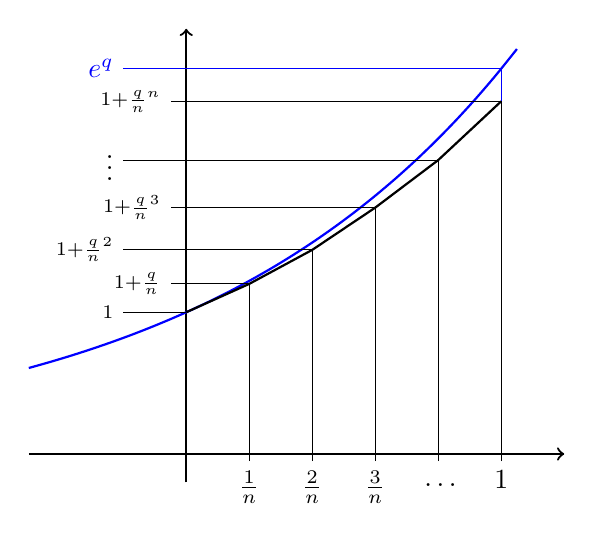
\begin{tikzpicture}[x=4.0cm,y=1.8cm]
    	\draw[thick,->] (-0.5,0) -- (1.2,0);
      \draw[thick,->] (0,-0.2) -- (0,3.0);
      %
      \draw[domain=-0.5:1.05,smooth,variable=\x,thick,blue] plot
      ({\x}, {exp(\x)});
      \draw[blue] (1.0,-0.05) -- (1.0,{exp(1.0)})
      -- (-0.2, {exp(1.0)}) node[left]{$e^q$};
      \draw (-0.2,1) node[left]{$\scriptstyle 1$} -- (0,1);
      \draw (0.2,-0.05) node[below]{$\frac 1 n$} -- (0.2,1.2)
      -- (-0.05,1.2) node[left]{$\scriptstyle 1+\frac q n$};
      \draw (0.4,-0.05) node[below]{$\frac 2 n$} -- (0.4,1.44)
      -- (-0.2,1.44) node[left]{$\scriptstyle\enclose{ 1+\frac q n}^2$};
      \draw (0.6,-0.05) node[below]{$\frac 3 n$} -- (0.6,1.738)
      -- (-0.05,1.738) node[left]{$\scriptstyle\enclose{1+\frac q n}^3$};
      \draw (0.8,-0.05) node[below]{$\rule{0mm}{2mm}\dots$} -- (0.8,2.0736)
      -- (-0.2,2.0736) node[left]{$\vdots$};
      \draw (1.0,-0.05) node [below] {$1$} -- (1.0,2.48832)
      -- (-0.05,2.48832) node[left]{$\scriptstyle\enclose{1+\frac q n}^n$};
      \draw[thick] (0,1) -- (0.2,1.2)
      -- (0.4,1.44) -- (0.6,1.738)
      -- (0.8,2.0736) -- (1.0,2.48832);
    \end{tikzpicture}
  \end{center}
  \caption{L'interesse composto.
  Se dividiamo l'intervallo $[0,1]$
  in $n$ parti (in figura $n=5$), al passo zero
  partiamo con un capitale pari ad $1$ e ad ogni
  passo di ampiezza $\frac 1 n$ moltiplichiamo
  il nostro capitale per $1+\frac q n$ (supponendo
  di avere un interesse pari a $q$ che
  nel tempo $\frac 1 n$ ci paga quindi $\frac q n$
  volte il nostro capitale).
  Dopo
  $n$ passi, cioè al tempo $1$, avremo
  un capitale pari a $\enclose{1+\frac q n}^n$.
  Se $n\to+\infty$ questa quantità tende ad $e^q$.}
  \label{fig:nepero}
\end{figure}


La funzione esponenziale è legata ad un modello di crescita che si trova spesso
in natura: la \emph{crescita esponenziale}%
\mymargin{crescita esponenziale}%
\index{crescita!esponenziale}.
Prendiamo come esempio una popolazione di batteri che cresce senza
limitazioni di spazio e di nutrimento oppure
pensiamo alla crescita di un capitale dovuto ad una rendita finanziaria.

Supponiamo che una popolazione che al tempo $t_0=0$
ammonta ad un certo numero $c$ di batteri, al tempo
$t>0$ raggiunga una numerosità $q(t,c)$.
Se lascio crescere la popolazione per un ulteriore
tempo $s>0$ troverò al tempo $t+s$ la stessa
popolazione che avrei al tempo $s$ se al tempo
zero fossi partito con la popolazione $q(t)$:
\[
  q(t+s,c) = q(s,q(t,c)).
\]
L'equazione precedente si chiama proprietà
di \emph{semigruppo}
\index{semigruppo}%
continuo.
Ma fissato $t$ la popolazione $q(t,c)$ deve
essere proporzionale a $c$ perché ogni batterio
ha la sua discendenza indipendentemente dalla numerosità
totale della popolazione. In pratica
si deve avere $q(t,c) = k(t) \cdot c$ per una opportuna
funzione $k(t)$ che non dipende da $c$.
Dunque
\[
  q(t+s,c)
  = q(s,q(t,c))
  = k(s) \cdot q(t,c)
  = k(s) \cdot k(t) \cdot c
\]
da cui
\[
  k(t+s) = k(s) \cdot k(t).
\]
In base al teorema~\ref{th:isomorfismo}
possiamo affermare
che $k(t)$ è una funzione esponenziale $k(t)=a^t$
per una qualche costante $a$.
La costante $a$ può essere determinata mediante la formula:
\[
  a = k(1) = \frac{q(1,c)}{c}
\]
ma questa espressione non ha un preciso significato fisico in quanto
dipende dall'unità di tempo scelta.

La costante a cui possiamo dare significato è invece l'aumento relativo
istantaneo della popolazione. Possiamo infatti supporre che
se lasciamo la popolazione crescere per un tempo $\Delta t$ molto piccolo,
si otterrà un aumento di popolazione proporzionale al tempo $\Delta t$
e alla popolazione:%
\mynote{stiamo qui anticipando il concetto di derivata}
\begin{equation}\label{eq:488464}
  q(\Delta t,c) = c + r c \Delta t = (1+r \Delta t) c.
\end{equation}
La costante $r$ rappresenta quindi l'aumento
relativo istantaneo della popolazione (nel caso dell'investimento
$r$ sarebbe il tasso di interesse istantaneo).
Questa definizione ha senso
quando $\Delta t$ è piccolo in quanto non tiene conto del fatto che
nell'intervallo di tempo $[t,t+\Delta t]$ la popolazione che si
è aggiunta genera anch'essa nuova popolazione (ovvero l'interesse
accumulato genera anch'esso interesse\mynote{%
In effetti la scoperta della costante $e$
è dovuta a Jacob Bernoulli (1655--1705) vedi note storiche 
a pag~\pageref{note:Bernoulli}}).

Per calcolare l'aumento della popolazione su tempi ``grandi'' possiamo
suddividere gli intervalli temporali in $n$ intervallini di ampiezza
$\Delta t$ e applicare in ognuno di essi la relazione \eqref{eq:488464}.
Si trova:
\begin{align*}
 q(\Delta t,c) &= c(1+r\Delta t) \\
 q(2\Delta t,c) &= q(\Delta t,c) (1+r\Delta t)  = c(1+r\Delta t)^2\\
 &\vdots \\
 q(n\Delta t) &= c(1+r\Delta t)^n.
\end{align*}
Dunque, ponendo $\Delta t=t/n$ si ha
\[
  q(t,c) = c\enclose{1+r\frac{t}{n}}^n
\]
in particolare per $t=1/r$ si ottiene:
\[
  q(1/r,c) = c\enclose{1+\frac{1}{n}}^n
\]
e ricordando che $q(t,c)=c a^t$ otteniamo:
\[
  a^{\frac 1 r} = \enclose{1+\frac{1}{n}}^n.
\]
Se per $n\to +\infty$ (che corrisponde a $\Delta t \to 0$)
la quantità sul lato destro tende ad un numero $e$ (che chiameremo costante
di Nepero) avremo allora
\[
  a = e^r, \qquad q(t,c) = c e^{rt}
\]
che è la relazione che lega le due costanti $a$ e $r$ che definiscono
la crescita esponenziale.

Risulta in effetti valido il seguente.

\begin{theorem}[costante di Nepero]
\mymark{**}%
\label{th:5767684}
La successione
\[
  a_n = \enclose{1+\frac 1 n}^n
\]
è crescente e limitata, dunque è convergente.
\end{theorem}
%
Per dimostrare il teorema precedente ci serve 
preliminarmente il seguente risultato.
%
\begin{theorem}[disuguaglianza di Bernoulli]
  \label{th:disuguaglianza_bernoulli}%
  \mymark{**}%
  \mymargin{disuguaglianza di Bernoulli}%
  \index{Bernoulli!disuguaglianza di}%
  \index{disuguaglianza!di Bernoulli}%
  Se $x > -1$ e $n\in \NN$ si ha
  \begin{equation}
  \label{eq:bernoulli}
  (1+x)^n \ge 1 + nx.
  \end{equation}
  \end{theorem}
  %
  \begin{proof}
  \mymark{**}
  Dimostriamo che vale~\eqref{eq:bernoulli}
  per induzione su $n$.
  Per $n=0$ la disequazione \eqref{eq:bernoulli} diventa $1\ge 1$
  ed è quindi verificata.
  Se~\eqref{eq:bernoulli}
  è verificata per un certo $n$
  moltiplicando ambo i membri per $1+x > 0$ si ottiene
  \[
  (1+x)^{n+1} \ge (1+x) (1+nx) = 1 + (n+1)x + n x^2
  \ge 1 + (n+1)x
  \]
  che è proprio la disuguaglianza~\eqref{eq:bernoulli}
  con $n+1$ al posto di $n$.
  \end{proof}
%
\begin{proof}[Dimostrazione del teorema~\ref{th:5767684}]
Dimostriamo innanzitutto che $a_n$ è crescente, cioè che
per ogni $n\ge 2$ si ha $a_n \ge a_{n-1}$.
E' chiaro che $a_n>0$ per ogni $n$,
quindi ci riconduciamo a
verificare che $\frac{a_n}{a_{n-1}} \ge 1$.

Si ha
\begin{align*}
\frac{a_n}{a_{n-1}}
&= \frac{\enclose{1+\frac 1 n}^n}{\enclose{1+\frac 1 {n-1}}^{n-1}}
= \frac{\enclose{\frac{n+1}{n}}^n}{\enclose{\frac{n}{n-1}}^{n-1}}\\
&= \enclose{\frac{n+1}{n}\cdot\frac{n-1}{n}}^n \cdot \frac{n}{n-1}
= \enclose{\frac{n^2- 1}{n^2}}^n \cdot \frac{n}{n-1}
\end{align*}
Osserviamo ora che la disuguaglianza di Bernoulli, 
teorema~\ref{th:disuguaglianza_bernoulli},
garantisce
\[
  \enclose{\frac{n^2 -1}{n^2}}^n
  = \enclose{1-\frac{1}{n^2}}^n
  \ge 1 - \frac{n}{n^2} = 1 - \frac{1}{n} = \frac{n-1}{n}
\]
da cui si ottiene, come volevamo, $a_n / a_{n-1} \ge 1$ cioè
$a_n$ è crescente.

Se ora consideriamo la successione
\[
  b_n = \enclose{1+\frac 1 n}^{n+1}
\]
osserviamo che si ha
\[
  b_n = \enclose{1+\frac 1 n}^n \cdot \enclose{1+\frac 1 n}
   = a_n\cdot \enclose{1+\frac 1 n} > a_n.
\]
Per dimostrare che $a_n$ è limitata sarà quindi sufficiente dimostrare
che $b_n$ è superiormente limitata. Vedremo ora che $b_n$ è decrescente (e quindi $a_n \le b_n \le b_1$ è superiormente limitata).

Procediamo in maniera analoga a quanto fatto per $a_n$:
\begin{align*}
\frac{b_{n-1}}{b_n}
& = \frac{\enclose{1+\frac{1}{n-1}}^n}{\enclose{1+\frac{1}{n}}^{n+1}}
  = \frac{\enclose{\frac{n}{n-1}}^n}{\enclose{\frac{n+1}{n}}^{n+1}}
  = \enclose{\frac{n}{n-1}\cdot\frac{n}{n+1}}^{n+1}\cdot\frac{n-1}{n} \\
& = \enclose{\frac{n^2}{n^2-1}}^{n+1} \cdot \frac{n-1}{n}
  = \enclose{1 + \frac{1}{n^2-1}}^{n+1} \cdot \frac{n-1}{n}.
\end{align*}
In base alla disuguaglianza di Bernoulli otteniamo
\[
  \enclose{1 + \frac{1}{n^2-1}}^{n+1}
  \ge 1 + (n+1) \cdot \frac{1}{n^2-1}
  = 1 + \frac{1}{n-1} = \frac{n}{n-1}.
\]
Mettendo insieme le due stime si ottiene dunque $b_{n-1}/b_n \ge 1$
che è quanto ci rimaneva da dimostrare.
\end{proof}

E' quindi giustificata la seguente.

\begin{definition}[costante di Nepero]
\mymark{***}
Definiamo la \emph{costante di Nepero}%
\mymargin{costante di Nepero}%
\index{costante!di Nepero}%
\index{$e$}%
\mynote{John Napier (1550-1617) vedi note storiche a pag~\pageref{nota:Nepero}}%
\[
  e = \lim_{n\to +\infty} \enclose{1+\frac 1 n}^n,
  \qquad n\in\NN.
\]
\end{definition}

Sapendo che
\[
  \enclose{1+\frac 1 n}^n \le e \le \enclose{1+\frac 1 n}^{n+1}
\]
e ponendo $n=1$ otteniamo $2\le e \le 4$.

\begin{exercise}\label{ex:4876765}
Posto $a_n = \frac{n^n}{n!}$ mostrare che $\frac{a_{n+1}}{a_n} \to e$.
\end{exercise}


\begin{theorem}[limiti che si riconducono al numero $e$]
\mymargin{limiti che si riconducono al numero $e$}%
\index{limiti che si riconducono al numero $e$}
Si ha 
\[
\lim_{x\to 0}  \enclose{1 + x}^{\frac 1 {x}} = e.
\]
\end{theorem}
%
\begin{proof}
  Iniziamo col dimostrare che 
  \begin{equation}\label{eq:2373793}
    \lim_{x\to +\infty} \enclose{1+\frac 1 x}^x = e.
  \end{equation}
  Ogni numero reale $x$ è compreso tra due interi consecutivi:
  \[
      \lfloor x \rfloor \le x \le \lfloor x\rfloor + 1
  \]
  e dunque
  \[
    1+\frac{1}{\lfloor x\rfloor +1 } 
    \le 1 + \frac 1 x 
    \le 1 + \frac 1 {\lfloor x\rfloor} 
  \]
  da cui 
  \begin{equation}\label{eq:48675248}
    \enclose{1+\frac{1}{\lfloor x\rfloor +1 }}^{\lfloor x\rfloor} 
    \le \enclose{1 + \frac 1 x }^x
    \le \enclose{1 + \frac 1 {\lfloor x\rfloor}}^{\lfloor x\rfloor +1}. 
  \end{equation}
  Per calcolare il limite della espressione a sinistra 
  operiamo il cambio di variabile $n=\lfloor x\rfloor + 1$ per 
  ottenere:
  \begin{align*}
  \lim_{x\to+\infty} \enclose{1+\frac{1}{\lfloor x\rfloor +1 }}^{\lfloor x\rfloor}
  &= \lim_{n\to +\infty} \enclose{1+\frac 1 n}^{n-1}\\
  &= \lim_{n\to +\infty} \frac{\enclose{1+\frac 1 n}^{n}}{1+\frac 1 n}
   = \frac{e}{1} = e.
  \end{align*}
  Similmente per quanto riguarda il limite della espressione a destra 
  si può operare il cambio di variabile $n=\lfloor x\rfloor$:
  \begin{align*}
    \enclose{1 + \frac 1 {\lfloor x\rfloor}}^{\lfloor x\rfloor +1}
    &= \lim_{n\to+\infty} \enclose{1+\frac 1 n}^{n+1} \\
    &= \lim_{n\to+\infty} \enclose{1+\frac 1 n}^n 
    \cdot \enclose{1 + \frac 1 n} 
    = e \cdot 1 = e.
  \end{align*}
  Dunque per il teorema dei due carabinieri otteniamo
  che anche l'espressione 
  al centro in~\eqref{eq:48675248} tende ad $e$.
  Come conseguenza, tramite il cambio di variabile $x\mapsto \frac 1 x$
  si ottiene 
  \[
  \lim_{x\to 0^+}\enclose{1+x}^{\frac 1 x} = e.  
  \]

  Consideriamo ora il limite per $x\to -\infty$ 
  della solita espressione. 
  Tramite il cambio di variabile $y=-x$ si ha 
  \begin{align*}
  \lim_{x\to -\infty} \enclose{1+\frac{1}{x}}^x 
  &= \lim_{y\to +\infty} \enclose{1 - \frac 1 y}^{-y}
   = \lim_{y\to +\infty} \enclose{\frac {y-1} y}^{-y}\\
  &= \lim_{y\to +\infty} \enclose{\frac{y}{y-1}}^y
   = \lim_{y\to +\infty} \enclose{1 + \frac{1}{y-1}}^y\\
  &= \lim_{y\to +\infty} \enclose{1 + \frac{1}{y-1}}^{y-1}
    \cdot\enclose{1+\frac 1 {y-1}} 
    = e\cdot 1 = e.\\
  \end{align*}
  Di conseguenza, facendo il cambio di variabile $x\mapsto \frac 1 x$ 
  si ottiene
  \[
  \lim_{x\to 0^-} \enclose{1+x}^{\frac 1 x} = e.
  \]
  Mettendo insieme limite destro e limite sinistro si ottiene 
  infine il limite completo per $x\to 0$. 
\end{proof}
%
\begin{corollary}%
\label{cor:limite_notevole_ex}%
\mymark{**}%
Per ogni $x\in \RR$ si ha
\[
  \lim_{n\to +\infty} \enclose{1+ \frac x n}^n = e^x.
\]
\end{corollary}
%
\begin{proof}
Infatti, per il teorema precedente, posto $a_n = x/n$ si ha
\[
\lim_{n\to +\infty}\enclose{1+\frac x n}^{\frac n x} = e.
\]
Ma allora
\[
\enclose{1+ \frac x n}^n = \enclose{\enclose{1+\frac x n}^{\frac n x}}^x
\to e^x
\]
\end{proof}

\begin{definition}[logaritmi naturali]
Vedremo che il numero $e$ risulta essere una base naturale per la funzione
esponenziale e di conseguenza per il logaritmo. Il logaritmo in base
$e$ viene chiamato \emph{logaritmo naturale}%
\mymargin{logaritmo naturale}%
\index{logaritmo!naturale} e viene indicato con $\ln = \log_e$.
\end{definition}

\mynote{%
In alcuni testi si utilizza l'operatore $\log$, indicato senza una base esplicita,
ma la definizione non è completamente condivisa.
In certi testi (per lo più in ambito matematico)
si definisce $\log  = \ln = \log_e$,
in altri testi si considera $\log = \log_{10}$.
}

\begin{corollary}[limiti notevoli]\label{cor:limite_notevole_e}
\mymark{*}%
Si ha
\begin{gather}
 \lim_{x\to 0} \frac{\ln \enclose{1+ x}}{x} = 1; \\
 \lim_{x\to 0} \frac{e^x-1}{x} = 1.
\end{gather}
\end{corollary}
%
\begin{proof}
Per quanto riguarda il logaritmo ci si riconduce al teorema precedente
osservando che:
\[
  \frac{\ln(1+x)}{x}
  = \ln \enclose{(1+x)^{\frac 1 {x}}}
  \to \ln e = 1.
\]
Per l'esponenziale ci si riconduce al logaritmo
osservando che posto
\[
  y = e^x-1
\]
se $x\to 0$ anche $y\to 0$ e quindi si ha:
\[
\frac{e^{x}-1}{x} = \frac{y}{\ln(1+y)} \to 1.
\]

\end{proof}

\begin{exercise}
Mostrare che
\begin{gather*}
  \lim_{n\to+\infty} n^n\cdot \enclose{\frac{n+1}{n^2+1}}^n = e; \\
  \lim_{n\to+\infty} n\cdot \ln\enclose{1 + \frac 1 n} = 1; \\
  \lim_{n\to+\infty} \enclose{1-\frac{n+1}{n!}}^{(n-1)!} = \frac 1 e; \\
  \lim_{n\to+\infty} n \cdot \enclose{\sqrt[n]{2}-1} = \ln 2.
\end{gather*}
\end{exercise}

%%%%%%%%%%%%%%%%%%%
%%%%%%%%%%%%%%%%%%%
%%%%%%%%%%%%%%%%%%%
%%%%%%%%%%%%%%%%%%%
\subsection{criteri del rapporto e della radice}

Succede spesso di dover determinare il limite
del rapporto di due successioni che tendono entrambe a infinito
oppure entrambe a zero.
In queste situazioni il teorema del limite del rapporto non
si applica in quanto siamo di fronte ad una forma indeterminata.
Dovremo quindi capire quale delle due successioni
tende a infinito o a zero ``più velocemente''.

I teoremi che seguono si basano (in maniera più o meno implicita)
sull'andamento della successione geometrica:
\[
  a_n = q^n
\]
dove $q>0$ è una costante fissata.
Dalle proprietà della funzione esponenziale 
sappiamo che se $q>1$ si ha $q^n\to \infty$.
Se $q=1$ chiaramente $q^n=1\to 1$
e se $q<1$ si ha $q^{-1}>1$ e quindi $q^{-n} \to +\infty$
da cui $q^n \to 0$.

\begin{theorem}[criterio del rapporto]
\label{th:criterio_rapporto}
\index{criterio!del rapporto per le successioni}
\index{rapporto!criterio del}
  Sia $a_n$ una successione reale a termini positivi
  $a_n > 0$ tale che esista il limite del rapporto di due termini consecutivi:
  \[
     \frac{a_{n+1}}{a_n} \to \ell \in [0,+\infty].
  \]
  Se $\ell < 1$ allora $a_n \to 0$, se $\ell >1$ allora $a_n \to +\infty$.
\end{theorem}
%
%
% \begin{proof}\mynote{%
%   la dimostrazione di questo teorema si potrebbe fare in maniera
%   molto simile alla dimostrazione del teorema~\ref{th:criterio_radice}
%   senza tirare in ballo il teorema~\ref{th:criterio_cesaro} che è decisamente più complesso.
%   }
% Grazie al teorema~\ref{th:criterio_cesaro} sappiamo
% che $\sqrt[n]{a_n}\to \ell$ e quindi il risultato
% segue direttametne dal teorema~\ref{th:criterio_radice}.
% \end{proof}
%

\begin{proof}
Supponiamo sia $\ell<1$. Posto $q=(1+\ell)/2$ si ha $\ell < q < 1$ 
e posto $\eps=q-\ell>0$ per la definizione di limite $\frac{a_{n+1}}{a_n}\to \ell$ 
dovrà esistere un $N\in \NN$ tale
che per ogni $n\ge N$ si abbia:
\[
  \frac{a_{n+1}}{a_n} < \ell + \eps = q
\]
ovvero $a_{n+1} < q \cdot a_n$. In particolare si avrà:
\begin{align*}
  a_{N+1} &< q \cdot a_N \\
  a_{N+2} &< q \cdot a_{N+1} < q^2\cdot a_N \\
  a_{N+3} &< q \cdot a_{N+2} < q^3\cdot a_N \\
  \vdots
\end{align*}
ed è chiaro che per induzione potremo dimostrare che per
ogni $k\in \NN$ si ha
\[
  a_{N+k} < q^k\cdot a_N.
\]
Osserviamo però che $q^k \cdot a_N \to 0$ per $k\to +\infty$
in quanto $q<1$ e quindi $q^k \to 0$. 
Dunque, tolti i primi $N$ termini, la successione $a_n$ tende a zero. 
Ma i primi $N$ termini non influenzano né il carattere né il limite 
della successione e quindi l'intera successione $a_n$ tende a zero.

Il caso $\ell>1$ si fa in maniera analoga. Si sceglie $q$ tale
che $1<q<\ell$ e si trova, in maniera analoga al caso precedente,
che per un certo $N\in \NN$ e per ogni $k\in \NN$ si ha
\[
  a_{N+k} > q^k \cdot a_N \to +\infty.
\]
\end{proof}

Osserviamo che, nel teorema precedente (ma anche nel criterio della radice teorema~\ref{th:criterio_radice}),
non si può concludere alcunché nel
caso in cui sia $\ell = 1$.
Ad esempio le due successioni $a_n = 1/n$ e $b_n = n$
hanno limiti diversi ($a_n \to 0$, $b_n\to +\infty$) ma per entrambe
il limite del rapporto di termini consecutivi tende ad $\ell=1$.

\begin{exercise}
Mostrare che
\begin{gather*}
  \lim \frac{n!}{n^n} = 0 \\
  \lim \frac{(2n)!}{(2n)^n} = +\infty
\end{gather*}
\end{exercise}

\begin{theorem}[criterio della radice]
\label{th:criterio_radice}%
\mymark{***}%
\mymargin{criterio della radice}%
\index{criterio!della radice per successioni}%
Sia $a_n$ una successione a termini non negativi, $a_n\ge 0$, tale che
\[
  \sqrt[n]{a_n} \to \ell
\]
con $\ell \in \bar \RR$.
Allora se $\ell<1$ si ha $a_n \to 0$ se invece $\ell > 1$ si ha $a_n \to +\infty$.
\end{theorem}
%
\begin{comment}
\begin{proof}
\mymark{**}
Consideriamo prima il caso $\ell < 1$.
Se $\lim \sqrt[n]{a_n} = \ell$ significa che per ogni $\eps>0$ la successione
$\sqrt[n]{a_n}$ risulta definitivamente minore di $\ell +\eps$.
Scegliendo opportunamente $\eps$ (ad esempio $\eps = (1-\ell)/2$) si potrà
avere $q = \ell+\eps < 1$. Dunque avremo definitivamente $\sqrt[n]{a_n}< q$
ovvero $a_n < q^n$. Per ipotesi $a_n\ge 0$
e quindi, tolto un numero finito di termini, si ottiene $0 \le a_n < q^n \to 0$
da cui $a_n \to 0$ (in quanto l'aver tolto un numero finito di termini non
cambia né il carattere né il limite della successione).

Se $\ell>1$ si potrà procedere in maniera analoga. Esisterà $q$ con $1 < q < \ell$ tale che definitivamente $\sqrt[n]{a_n} > q$ da cui $a_n > q^n \to +\infty$.
\end{proof}
\end{comment}

\begin{proof}
  Si può osservare che
  \[
    a_n = \enclose{\sqrt[n]{a_n}}^n
     = e^{n \cdot \ln \sqrt[n]{a_n}}.
  \]
  Se $\ell <1$ allora il logaritmo tende ad un numero negativo,
  l'argomento dell'esponenziale tende a $-\infty$ e quindi l'esponenziale tende a zero.

  Se invece $\ell>1$ il logaritmo tende ad un numero positivo e quindi l'esponenziale tende a $+\infty$.
\end{proof}

%%%%%
%%%%%
\section{ordini di infinito, equivalenza asintotica}
%%%%%
%%%%%

\begin{definition}[ordine di infinito/infinitesimo]%
  \label{def:ordine_infinito}%
  \mymark{***}%
  \mymargin{ordine di infinito/infinitesimo}%
\index{ordine di infinito/infinitesimo}%
  \index{ordine!di infinito}%
  \index{infinito}%
  \index{infinitesimo}%
  Sia $A\subset \RR$, $f,g\colon A \to (0,+\infty)$.
  Sia $x_0\in \bar \RR$ un punto di accumulazione di $A$.
  \begin{enumerate}
  \item
  Diremo che
  per $x\to x_0$ la funzione $f$ è \emph{molto più piccola}
  della funzione $g$ e scriveremo $f(x) \ll g(x)$ se vale
  \mymargin{$\ll$}%
\index{$\ll$}
  \[
  \frac{f(x)}{g(x)} \to 0, \qquad \text{per $x\to x_0$}
  \]
  diremo invece che $f$ è \emph{molto più grande}
  di $g$ e scriveremo $f(x) \gg g(x)$ se
  \mymargin{$\gg$}%
\index{$\gg$}
  \[
  \frac{f(x)}{g(x)} \to +\infty, \qquad \text{per $x\to x_0$.}
  \]
  \item
  Diremo infine che $f$ e $g$
  sono \emph{asintoticamente equivalenti}%
\mymargin{equivalenza asintotica}%
\index{asintoticamente equivalenti}
  \mymargin{equivalenza asintotica}%
\index{equivalenza!asintotica}%
  per $x\to x_0$
  e scriveremo $f(x) \sim g(x)$ se
  \mymargin{$\sim$}%
\index{$\sim$}
  \[
  \frac{f(x)}{g(x)} \to 1, \qquad \text{per $x\to x_0.$}
  \]
  \end{enumerate}
\end{definition}
  
Ad esempio è facile verificare che se $\alpha > \beta > 0$
allora $x^\alpha \gg x^\beta$ per $x\to +\infty$
mentre $x^\alpha \ll x^\beta$ per $x\to 0^+$.
Analogamente se $a>b>1$ allora $a^x\gg b^x$ per $x\to +\infty$
mentre $a^x \ll b^x$ per $x\to -\infty$.

E' molto facile verificare che le relazioni
$\ll$ e $\gg$ sono una l'inversa dell'altra
e soddisfano la proprietà transitiva
mentre la relazione $\sim$ soddisfa la proprietà simmetrica
e la proprietà transitiva.

\begin{theorem}[ordini di infinito]
\label{th:ordine_infinito}%
\mymargin{ordini di infinito}%
\index{ordini di infinito}%
\mymark{***}%
Siano $a>1$ e $\alpha>0$. Per $n\to +\infty$, $n\in\NN$
si ha
\[
  n^\alpha \ll a^n \ll n! \ll n^n
\]
e per $x\to +\infty$, $x\in \RR$ si ha 
\[
\log_a x \ll x^\alpha \ll a^x.
\]
\end{theorem}
%
\begin{proof}
\mymark{**}
Cominciamo col mostrare che $a^n \ll n!$
applicando il criterio del rapporto alla successione $\frac{a^n}{n!}$:
\[
\frac{\displaystyle \frac{a^{n+1}}{(n+1)!}}{\displaystyle \frac{a^n}{n!}}
= \frac{a^{n+1}}{a^n}\cdot \frac{n!}{(n+1)!}
= a \cdot \frac {1}{n + 1} \to 0 < 1.
\]
Dunque si ha, come richiesto, $a^n / n! \to 0$.
Si procede in modo analogo per mostrare che $n! \ll n^n$:
\begin{align*}
\frac{(n+1)!}{n!}\cdot \frac{n^n}{(n+1)^{n+1}}
&= (n+1) \cdot \enclose{\frac{n}{n+1}}^n \frac {1}{n+1}\\
&= \frac{1}{\enclose{1+\frac 1 n}^n} \to \frac 1 e < 1.
\end{align*}
  
Per dimostrare che
$n^\alpha \ll a^n$
si può procedere con il criterio del rapporto, come nei casi precedenti:
\[
\frac{(n+1)^\alpha}{n^\alpha}\cdot \frac{a^n}{a^{n+1}}
= \frac 1 a \cdot \enclose{\frac{n+1}{n}}^\alpha \to \frac 1 a \cdot 1^\alpha = \frac 1 a < 1
\]
da cui $n^\alpha / a^n \to 0$.

Per $x\in \RR$,
cerchiamo di ricondurci ad una successione a valori interi.
Osserviamo che si ha
\[
\lfloor x \rfloor
\le x
\le \lfloor x \rfloor + 1
\]
da cui, per monotonia,
\[
\lfloor x \rfloor^\alpha
\le x^\alpha
\le (\lfloor x \rfloor + 1)^\alpha
= \lfloor x \rfloor^\alpha \enclose{1+ \frac{1}{\lfloor x \rfloor}}^\alpha
\]
e
\[
a^{\lfloor x \rfloor}
\le a^{x}
\le a^{\lfloor x \rfloor + 1}
= a \cdot a^{\lfloor x \rfloor}.
\]
Dunque
\[
\frac{\lfloor x \rfloor^\alpha}{a \cdot a^{\lfloor x \rfloor}}
\le \frac{x^\alpha}{a^{x}}
\le \frac{\lfloor x \rfloor^\alpha \enclose{1+ \frac{1}{\lfloor x \rfloor}}^\alpha}
    {a^{\lfloor x \rfloor}}.
\]
Ma ora, se $x\to +\infty$ sapendo che $n = \lfloor x\rfloor \to +\infty$ 
possiamo effettuare un cambio di variabile nel limite
\[
\lim_{x\to +\infty} \frac{\lfloor x \rfloor^\alpha}{a^{\lfloor x \rfloor}} 
= \lim_{n\to+\infty} \frac{n^\alpha}{a^n} = 0
\qquad
\text{e}
\qquad
\lim_{x\to+\infty} \frac{\lfloor x \rfloor^\alpha }
    {a^{\lfloor x \rfloor}} 
= \lim_{n\to+\infty} \frac{n^\alpha}{a^n} = 0
\]
da cui segue che $\frac{x^\alpha}{a^{x}}\to 0$.

Per dimostrare l'ultima relazione, $\log_a x\ll x^\alpha$,
operiamo il cambio di variabile $y = \alpha \cdot \log_a x$
cosicché $a^y = x^\alpha$.
Notiamo che se $x\to +\infty$
anche $y \to +\infty$.
Dunque, per le proprietà precedenti,
sappiamo che $y \ll a^y$ e dunque
\[
\frac{\log_a x}{x^\alpha}
= \frac{1}{\alpha}\cdot\frac{y}{a^{y}} \to 0.
\]
\end{proof}

Le notazioni e gli
ordini di infinito individuati nel teorema precedente
sono strumenti molto utili nel calcolo dei limiti.

L'equivalenza asintotica
si mantiene per prodotto e rapporto:
se $f\sim F$ e $g\sim G$ allora
\[
 f \cdot g \sim F \cdot G,
 \qquad
 \frac{f}{g} \sim \frac{F}{G}.
\]
Osserviamo inoltre che se
$f \sim g$ e se $f\to \ell$ allora
anche $g\to \ell$.
Se poi $\ell\in(0,+\infty)$
la relazione $f\sim \ell$ è equivalente ad $f\to \ell$.

Per quanto riguarda la somma
è facile verificare che se $f\ll g$ allora
$(f+g) \sim g$ in quanto
\[
  \frac{f + g}{g} = \frac{f}{g} + 1 \to 1.
\]

In un limite in cui compaiono somme di termini
di ordini diversi potremo allora raccogliere i termini di ordine
massimo per individuare il limite, come facciamo
nel seguente.

\begin{example}
Calcolare il limite
\[
\lim_{n\to+\infty}
\frac{2n^4 + 3^n - 3 \ln n}{n! - 3\sqrt n}.
\]
\end{example}
\begin{proof}[Svolgimento.]
Si ha
\[
\frac{2n^4 + 3^n - 3 \ln n}{n! - 3\sqrt{n}}
= \frac
{3^n \cdot \enclose{2\frac{n^4}{3^n}+ 1 - 3\frac{\ln n}{3^n}}}
{n!\cdot \enclose{1-3\frac{\sqrt n}{n!}}}
\]
e ricordando che risulta (teorema~\ref{th:ordine_infinito})
\[
n^4 \ll 3^n, \qquad
\ln n \ll 3^n, \qquad
\sqrt n \ll n!, \qquad
3^n \ll n!
\]
avremo
\[
\frac{2n^4 + 3^n - 3 \ln n}{n! - 3\sqrt{n}}
\sim \frac{3^n}{n!} \to 0.
\]
\end{proof}


\begin{exercise}
Calcolare i seguenti limiti
\begin{gather*}
  \lim_{n\to +\infty} \frac{\displaystyle \ln\sqrt{n^2+n^n}}
  {\displaystyle e^{1 + \ln n}\cdot \ln(n^2-n\sqrt n)}, \qquad
  \lim_{n\to +\infty} \frac{\sqrt{n! + 2^n}}{3^n}, \\
  \lim_{n\to +\infty} \frac{\sqrt{(2n)!}}{n^n}, \qquad
  \lim_{n\to +\infty} \sqrt[n]{e^n + \sqrt{10^n}}.
\end{gather*}
\end{exercise}

\begin{exercise}
  Dimostrare che $\sqrt[n]{n}\to 1$ per $n\to +\infty$.
\end{exercise}



%%%%%%%%%%%
%%%%%%%%%%%
\section{successioni estratte}
%%%%%%%%%%%
%%%%%%%%%%%

\begin{definition}[sottosuccessione]
\mymark{*}
Se $a_n$ è una successione e $n_k$ è una successione strettamente crescente i cui valori sono numeri naturali, allora la successione
$b_k = a_{n_k}$ si dice essere una \emph{sottosuccessione}%
\mymargin{sottosuccessione}%
\index{sottosuccessione} di $a_n$
(o anche \emph{successione estratta} da $a_n$).
\end{definition}

Ricordando che una successione $a_n$ non è altro che una funzione
$\vec a\colon \NN \to \RR$, la successione $n_k$ corrisponde ad una funzione
$\vec n\colon \NN \to \NN$ e la sottosuccessione $a_{n_k}$ corrisponde alla
funzione composta $\vec a \circ \vec n$.

Si osservi che nella definizione precedente la variabile $n$ rappresenta
una variabile muta quando scriviamo la successione $a_n$, ma
rappresenta anche il nome della successione fissata $n_k$.
Questo sovraccarico
di significato è voluto e se usato correttamente rende più semplice
le notazioni, in quanto la successione $n_k$ viene sostituita alla
variabile $n$, con lo stesso nome, nella successione $a_n$.
La sottosuccessione $a_{n_k}$ risulta essere una successione nella variabile $k$, non nella variabile $n$.

\begin{example}
Sia $a_n = n^2$ la successione dei quadrati perfetti:
\begin{center}
\begin{tabular}{l|rrrrrrrrr}
$n$   & $0$ & $1$ & $2$ & $3$ & $4$  & $5$  & $6$  & \dots \\ \hline
$a_n$ & $0$ & $1$ & $4$ & $9$ & $16$ & $25$ & $36$ & \dots
\end{tabular}
\end{center}
Consideriamo la successione dei numeri pari $n_k = 2k$.
la corrispondente sottosuccessione dei quadrati perfetti
$b_k = a_{n_k}$
rappresenta la successione dei quadrati dei numeri pari:
\begin{center}
\begin{tabular}{l|rrrrrrrrr}
$k$       & $0$ & $1$ & $2$ & $3$ & $4$  & $5$  & $6$  & \dots \\ \hline
$n_k$ & $0$ & $2$ & $4$ & $6$ & $8$ & $10$ & $12$ & \dots \\
$a_{n_k}$ & $0$ & $4$ & $16$ & $36$ & $64$ & $100$ & $144$ & \dots
\end{tabular}
\end{center}
Si ha in pratica
  $b_k = a_{n_k} = a_{2k} = (2k)^2$.

Abbiamo in effetti \emph{estratto} alcuni dei termini della successione
originaria.
\end{example}

\begin{example}
Se $a_n = (-1)^n$ e $n_k=2k$ allora $a_{n_k} = 1$.
Vediamo quindi che una successione irregolare
può contenere una sottosuccessione regolare.
\end{example}

Osserviamo che se $\vec n\colon \NN\to \NN$ è una
funzione strettamente crescente
(cioè $n_k=\vec n(k)$ è una successione strettamente crescente di indici)
allora posto $A=\vec n(\NN)=\ENCLOSE{n_k\colon k\in \NN}$ si ha che
$\vec n \colon \NN \to A$ è una bigezione. Quindi $A$ è un insieme infinito.
Viceversa dato un qualunque insieme infinito $A\subset \NN$ esiste una
unica successione $\vec n\colon \NN \to A$ bigettiva e strettamente crescente:
basterà porre, per induzione,
$n_0 = \min A$, $n_1 = \min \ENCLOSE{n\in A \colon n > n_0}$
e, in generale,
 $n_{k+1} = \min\ENCLOSE{ n\in A \colon n > n_k}$.

Dunque possiamo identificare le sottosuccessioni di una successione
$\vec a \colon \NN \to \RR$ con le restrizioni ai sottoinsiemi infiniti di $\NN$.
Nell'esempio precedente, si è considerata la sottosuccessione
di tutti i termini con indice pari $n_k=2k$ per ottenere la sottosuccessione
$a_{n_k} = a_{2k}$. Si può equivalentemente pensare di prendere l'insieme di
tutti i numeri pari $A=2\NN$ e considerare la successione ristretta ai soli
indici pari:
\[
  a_0, a_2, a_4, \dots
\]
Se rinumeriamo gli indici pari usando tutti i numeri naturali otteniamo
la sottosuccessione $b_k=a_{n_k}$:
\[
  b_0 = a_0,\ b_1 = a_2,\ b_2 = a_4,\ \dots,\ b_k = a_{n_k},\ \dots
\]

\begin{lemma}[estratte monotone]%
\label{lem:estratte_monotone}%
Ogni successione $a_n\in \RR$ ha una estratta $a_{n_k}$ monotona.
Inoltre se $\sup a_n = +\infty$ c'è una estratta $a_{n_k}$
strettamente crescente che tende a $+\infty$.
\end{lemma}
%
\begin{proof}
Consideriamo l'insieme $P$ dei punti di ``picco'', ovvero degli indici
di quei termini della successione che sono maggiori o uguali a tutti i termini
seguenti:
\[
  P = \ENCLOSE{n\in \NN\colon m\ge n \implies a_n\ge a_m}.
\]
Se $P$ è finito
significa che esiste un indice $n_1\in \NN$ tale
che non ci sono picchi da $n_1$ in poi. In particolare $n_1$ non è un punto di
picco
quindi deve esistere $n_2>n_1$ tale che $a_{n_2}>a_{n_1}$.
Ma neanche $n_2$ è un punto di picco quindi deve esistere $n_3>n_2$ tale
che $a_{n_3}>a_{n_2}$... procedendo induttivamente si riesce quindi a definire
una successione $n_k$ di indici tali che $a_{n_k}$ risulta essere strettamente
crescente.

In particolare se $\sup a_n = +\infty$ siamo nella situazione precedente 
perché chiaramente in tal caso $P$ è vuoto visto che per ogni $n\in \NN$ 
deve esistere $m\in \NN$ tale che $a_m > \max\ENCLOSE{a_0, a_1, \dots a_n}$
e certamente $m>n$.

Se, viceversa, $P$ è infinito allora elencando in ordine i suoi elementi otterremo
una successione $n_1 < n_2 < n_3, \dots$ di indici ognuno dei quali corrisponde ad un valore
di picco. 
Se $j>k$ si ha dunque $n_j>n_k$ ed essendo $n_k\in P$ significa che
$a_{n_j} \le a_{n_k}$. 
Dunque la successione $a_{n_k}$ risulta essere decrescente.
\end{proof}


\begin{theorem}[Bolzano-Weierstrass]\label{th:Bolzano}
\label{th:bolzano_weierstrass}%
\mymark{***}%
\mymargin{Bolzano-Weierstrass}%
\index{Bolzano-Weierstrass}%
\index{teorema!di Bolzano-Weierstrass}%
Ogni successione $a_n$ ha una estratta regolare.
Più precisamente se $a_n$ è una successione limitata
allora esiste una sottosuccessione
$a_{n_k}$ convergente.
Se $a_n$ è una successione non limitata allora 
esiste una estratta $a_{n_k}$ divergente.
\end{theorem}
%
\begin{proof}
\mymark{***}
Cominciamo con il caso reale $a_n\in \RR$.
Il lemma~\ref{lem:estratte_monotone} garantisce 
che esiste una estratta $a_{n_k}$ monotona. 
Ma per il teorema~\ref{th:limite_monotona} concludiamo 
immediatamente che $a_{n_k}$ ha limite.
Se $a_n$ è limitata anche $a_{n_k}$ è limitata e quindi 
in tal caso il limite è finito e dunque la successione 
estratta è convergente.

Se $a_n$ non è superiormente limitata il lemma 
ci garantisce che l'estratta tende a $+\infty$ 
e dunque è divergente.
Per simmetria se $a_n$ non è inferiormente limitata 
esiste una estratta che tende a $-\infty$ e quindi anche in
questo caso l'estratta è divergente.

Se $a_n$ è una successione di numeri complessi, si potrà scrivere
$a_n = x_n + i y_n$ con
$x_n$ e $y_n$ successioni reali. Se $a_n$ è limitata significa che $\abs{a_n}$
è superiormente limitata. Ma risulta $\abs{x_n} \le \abs{a_n}$ e
$\abs{y_n}\le \abs{a_n}$ quindi se $a_n$ è limitata anche la parte reale
$x_n$ e la parte immaginaria $y_n$ sono successioni limitate.
Allora $x_n$ ammette una sotto-successione convergente $x_{n_k}$.
Ma $y_{n_k}$ è anch'essa limitata e quindi anch'essa ammette una
sotto-sotto-successione $y_{n_{k_j}}$ convergente.
Dunque la sotto-sotto-successione $a_{n_{k_j}}$ è convergente.

Se $a_n\in \CC$ non è limitata, applicando il teorema al suo modulo $\abs{a_n}$
troviamo che c'è una estratta $a_{n_k}$ tale che $\abs{a_{n_k}}\to +\infty$.
Ma questo significa che $a_{n_k}\to \infty \in \bar \CC$.
\end{proof}

%% \begin{comment}%% SECONDO METODO DIAGONALE DI CANTOR
%% 
%% Il seguente teorema è molto importante dal punto di vista
%% culturale, ma non verrà utilizzato nella teoria seguente.
%% 
%% \begin{theorem}[Cantor: secondo metodo diagonale]
%% \label{th:cantor_secondo}%
%% \mymargin{non numerabilità dei reali}%
%% \index{non numerabilità dei reali}%
%% \index{secondo metodo diagonale di Cantor}%
%% \index{Cantor}%
%% \index{teorema!di Cantor}%
%% L'insieme dei numeri reali non è numerabile: $\#\RR > \#\NN$.
%% \end{theorem}
%% %
%% \begin{proof}
%% E' sufficiente dimostrare che $\#[0,1] > \#\NN$ in quanto
%% chiaramente $\#\RR \ge \#[0,1]$.
%% Supponiamo per assurdo che esista una funzione biettiva $a\colon \NN \to [0,1]$.
%% Questa funzione corrisponde dunque ad una successione $a_n$.
%% Consideriamo l'intervallo $[0,1]$ e dividiamolo in tre intervalli  di lunghezza $1/3$: $[0,1/3]$, $[1/3,2/3]$, $[2/3,1]$. Il punto $a_0$ non può stare in tutti e tre questi intervalli. Sia $[A_0,B_0]$ un intervallo (dei tre) che non contiene $a_0$: $a_0 \not \in [A_0,B_0]$.
%% Dividiamo anche $[A_0,B_0]$ in tre intervalli di lunghezza $1/9$.
%% Almeno uno di questi tre intervalli, che chiamiamo $[A_1,B_1]$,
%% non contiene $a_1$: $a_1 \not \in [A_1,B_1]$.
%% Procediamo così all'infinito in maniera simile al teorema precedente.
%% Otterremo due successioni $A_n$, $B_n$ che soddisfano queste proprietà:
%% \begin{enumerate}
%% \item $A_n$ crescente, $B_n$ decrescente;
%% \item $0\le A_n \le B_n \le 1$;
%% \item $a_n \not \in [A_n, B_n]$;
%% \item $B_n - A_n = 1/3^{n+1}$.
%% \end{enumerate}
%% 
%% Essendo $A_n$ monotona e limitata, essa ha limite finito $\lim A_n = \ell$.
%% Fissato $n$ osserviamo che per ogni $k\ge n$ si ha
%% \[
%%   A_n \le A_k \le b_k \le B_n
%% \]
%% passando al limite in $k$ (con $n$ fissato) si ottiene
%% \[
%%   A_n \le \ell \le B_n
%% \]
%% che significa che $\ell \in [A_n, B_n]$ per ogni $n\in \NN$
%% (in particolare $\ell \in [0,1]$).
%% Visto che invece $a_n \not \in [A_n, B_n]$ risulta che per
%% ogni $n\in \NN$ si ha $\ell \neq a_n$.
%% Dunque il numero $\ell$ non è un termine della successione $a_n$
%% ovvero la funzione $a\colon \NN \to [0,1]$ non è suriettiva.
%% \end{proof}
%% \end{comment}


%%%%%%%%%%%%
%%%%%%%%%%%%
\subsection{punti limite}
%%%%%%%%%%%%
%%%%%%%%%%%%

\begin{theorem}[ponte di collegamento tra limiti di funzione e limiti di successione]%
\label{th:ponte}%
\mymark{***}%
Sia $A \subset \RR$, $f\colon A \to \RR$, sia $x_0$ un punto di accumulazione di $A$ e sia
$\ell \in [-\infty, +\infty]$.
Le due seguenti condizioni sono equivalenti:
\begin{enumerate}
\item $\displaystyle \lim_{x\to x_0} f(x) = \ell$;
\item per ogni successione $a_n\to x_0$ con $a_n\in A\setminus\ENCLOSE{x_0}$ risulta
\[
\lim_{n\to+\infty} f(a_n) = \ell. 
\]
\end{enumerate}
\end{theorem}
%
\begin{proof}
\mymark{***}
Se per $x\to x_0$ si ha $f(x)\to \ell$ e se $a_n \to x_0$ con $a_n\in A\setminus\ENCLOSE{x_0}$ la successione $f(a_n)$ non è altro che la composizione
della funzione $f$ con la funzione $n\mapsto a_n$. Si può quindi applicare
il teorema sul limite della funzione composta per ottenere che $f(a_n)\to \ell$.

Supponiamo viceversa di sapere che per ogni successione $a_n\to x_0$ si ha $f(a_n)\to \ell$. Vogliamo mostrare allora che $f(x)\to \ell$. Lo facciamo per assurdo: supponiamo che esista un intorno $U$ di $\ell$ tale che preso un qualunque intorno $V$ di $x_0$ non si abbia $f((A\setminus\ENCLOSE{x_0})\cap V)\subset U$.
Possiamo considerare per ogni $n\in \NN$ degli intorni $V_n$ sempre più piccoli. Ad esempio nel caso $x_0 \in \RR$ potremo scegliere $V_n = (x_0-1/n, x_0+1/n)$, nel caso $x_0 = +\infty$ si potrà scegliere $V_n = (n,+\infty]$ e nel caso $x_0=-\infty$ si sceglierà $V_n = [-\infty, -n)$.
Se per assurdo $f((A\setminus\ENCLOSE{x_0}\cap V_n))$ non fosse contenuto in $U$
significherebbe che per ogni $n\in\NN$ esisterebbe $a_n \in (A\setminus\ENCLOSE{x_0})\cap V_n$ tale che $f(a_n)\not \in U$. Ma allora $a_n$ risulterebbe essere una successione in
$A\setminus \ENCLOSE{x_0}$ con limite $x_0$
(in quanto per ogni intorno di $x_0$ esiste un $N$ tale che $V_N$ sia contenuto in tale intorno e per ogni $n>N$ si ha $V_n\subset V_N$)
ma $f(a_n)$ non potrebbe avere limite $\ell$
(essendo fuori dall'intorno $U$).
Ma questo nega l'ipotesi e conclude quindi la dimostrazione del teorema.
\end{proof}
\begin{proposition}[proprietà caratteristica della convergenza]
  \label{prop:convergenza}
Sia $f\colon A\subset \RR\to \RR$ e $x_0$ punto di accumulazione di $A$.
Sia $\ell\in \bar \RR$.
Se per ogni $a_n\to x_0$, $a_n\in A\setminus\ENCLOSE{x_0}$
esiste una estratta $a_{n_k}$ tale che $f(a_{n_k})\to \ell$ 
allora $f(x)\to \ell$ per $x\to x_0$.
\end{proposition}
%
\begin{proof}
  Se per assurdo non fosse $f(x) \to \ell$
  esisterebbe un intorno $U\in \B_\ell$
  per cui frequentemente $f(x) \not \in U$.
  Questo significa che esiste una successione
  $a_n\to x_0$ con $a_n\neq x_0$ tale che $f(a_n)\not \in U$.
  Ma allora da $f(a_n)$
  non è possibile estrarre una sottosuccessione
  che abbia limite $\ell$, e questo è contrario alle
  ipotesi.
\end{proof}

\begin{definition}[punti limite, limite superiore, limite inferiore]
  Sia $f\colon A\subset \RR \to \RR$ una funzione e $x_0\in \bar \RR$ 
  un punto di accumulazione per $A$.
  Una quantità $\ell\in \bar\RR$ si dice essere
  un \emph{punto limite}%
\mymargin{punto limite}%
\index{punto!limite} di $f(x)$ per $x\to x_0$ se 
  per ogni $U$ intorno di $\ell$ si ha $f(x)\in U$ 
  frequentemente per $x\to x_0$.
  
  Se denotiamo con $L\subset \bar\RR$ l'insieme
  dei punti limite possiamo definire il \emph{limite superiore} e il
  \emph{limite inferiore}
  \mymargin{limite superiore/inferiore}%
\index{limite!superiore/inferiore}
  rispettivamente come
  \[
  \limsup_{x\to x_0} f(x) = \sup L, \qquad
  \liminf_{x\to x_0} f(x) = \inf L.
  \]
\end{definition}
  
\begin{proposition}[base numerabile di intorni]%
  \label{prop:base_numerabile}%
  Per ogni $\ell\in \bar \RR$ esiste una successione $U_n$ di intorni di $\ell$ 
  con queste proprietà:
  \begin{enumerate}
    \item $U_{n+1}\subset U_n$;
    \item per ogni $U$ intorno di $\ell$ esiste $n\in \NN$ tale che $U_n\subset U$;
    \item se $a_n\in U_n$ allora $a_n\to \ell$.
  \end{enumerate}
\end{proposition}
\begin{proof}
Possiamo esplicitamente definire gli intorni $U_n$ come segue:
\[
  U_n = 
  \begin{cases}
    \openinterval{\ell-\frac 1 n}{\ell+\frac 1 n} & \text{se $\ell\in \RR$}\\ 
    \opencloseinterval{n}{+\infty} & \text{se $\ell=+\infty$}\\
    \closeopeninterval{-\infty}{-n} & \text{se $\ell=-\infty$.}
  \end{cases}
\]
La prima proprietà è ovviamente verificata.
La proprietà archimedea dei numeri reali garantisce la validità della seconda 
proprietà, da cui segue immediatamente la terza.
\end{proof}

\begin{proposition}[caratterizzazione dei punti limite]
  Sia $f\colon A\subset \RR\to \RR$, $x_0\in \bar \RR$ 
  punto di accumulazione per $A$. 
  Sono equivalenti:
  \begin{enumerate}
    \item $\ell$ è un punto limite di $f(x)$ per $x\to x_0$.
    \item esiste una successione $a_n\in A$, $a_n\neq x_0$, $a_n\to x_0$ 
    tale che $f(a_n)\to \ell$.
  \end{enumerate}
\end{proposition}
%
\begin{proof}
  Siano $U_n$ intorni di $\ell$ e $V_n$ intorni di $x_0$ definiti 
  come nella proposizione~\ref{prop:base_numerabile}.
  Se $\ell$ è un punto limite di $f(x)$ per $x\to x_0$ 
  significa che per ogni $U$ intorno di $\ell$ e per ogni $V$ 
  intorno di $x_0$ esiste $x\in A\cap V\setminus\ENCLOSE{x_0}$ 
  tale che $f(x)\in U$.
  Dunque per ogni $n$ esiste $a_n\in A \cap V\setminus\ENCLOSE{x_0}$ 
  tale che $a_n\in V_n$ e $f(a_n)\in U_n$. 
  Significa che $a_n\to x_0$, $a_n\neq x_0$, $f(a_n)\to \ell$ 
  come volevasi dimostrare.
  
  Viceversa se esiste una tale successione $a_n\to x_0$ allora 
  per ogni $V$ intorno di $x_0$ si ha definitivamente $a_n\in V$.
  E se $f(a_n)\to \ell$ per ogni $U$ intorno di $\ell$
  si ha anche $f(a_n)\in U$ definitivamente.
  Dunque esiste $n$ tale che $a_n\in V$ e $f(a_n)\in U$ confermando 
  quindi che $f(x)\in U$ frequentemente. 
\end{proof}

Molto spesso considereremo i punti limite di una successione $a_n$
per $n\to +\infty$.
In tal caso la caratterizzazione precedente ci dice che $\ell$ 
è un punto limite di $a_n$ per $n\to+\infty$ se esiste 
una successione di indici $n_k\to+\infty$ tale che $a_{n_k}\to \ell$.
Potremmo anche supporre $n_k$ strettamente crescente in quanto se 
$n_k\to \infty$ possiamo estrarre da $n_k$ una sottosuccessione 
strettamente crescente. 
Dunque l'insieme dei punti limite di una successione $a_n$ 
corrisponde all'insieme dei limiti di tutte le possibili 
sottosuccessioni di $a_n$.

\begin{example}
  La successione $a_n=(-1)^n$ ha due punti limite:
  \[
    \limsup_{n\to +\infty}(-1)^n = 1, \qquad \liminf_{n\to+\infty} (-1)^n = -1.
  \]
  Infatti la sottosuccessione dei termini con indice pari è costante $1$ mentre
  quella dei termini di indice dispari è costante $-1$.
  Non ci possono essere altri punti limite perché se ci fosse $a_{n_k}\to \ell$
  allora certamente $a_{n_k}=1$ frequentemente oppure $a_{n_k}=-1$
  frequentemente da cui o $\ell=1$ oppure $\ell=-1$.
\end{example}
%
\begin{example}
  Visto che $\#\QQ=\#\NN$ esiste una funzione $\vec a \colon \NN \to \QQ$
  surgettiva. Utilizzando la proprietà di densità dei numeri razionali
  si può dimostrare che l'insieme dei punti limite della corrispondente successione
  $a_n = \vec a(n)$ è tutto $\bar \RR$.
\end{example}

\begin{exercise}
  Si consideri la successione $a_n = \sqrt n -\lfloor \sqrt n\rfloor$.
  Calcolare 
  \[
    \liminf_{n\to+\infty} a_n, \qquad 
    \limsup_{n\to+\infty} a_n.
  \]
  Qual è l'insieme dei punti limite di $a_n$ per $n\to +\infty$?
\end{exercise}

%
\begin{theorem}[proprietà del limite superiore/inferiore]
Sia $f\colon A\subset \RR \to \RR$ e sia $x_0$ un punto di accumulazione per $A$.
Sia $L$ l'insieme dei punti limite di $f(x)$ per $x\to x_0$. 
Allora:
\begin{enumerate}
  \item %1
  $L\neq \emptyset$;

  \item %2
  $\displaystyle\limsup_{x\to x_0} f(x) \ge \liminf_{x\to x_0} f(x)$;

  \item %3
  se $\displaystyle\limsup_{x\to x_0} f(x) = \liminf_{x\to x_0} f(x) = \ell$ 
  allora $\displaystyle\lim_{x\to x_0} f(x) = \ell$;

  \item %4
  l'insieme dei punti limite è chiuso per passaggio al limite:
  se $\ell_k\in L$ e $\ell_k \to \ell$ per qualche $\ell \in \bar \RR$ 
  allora $\ell \in L$;

  \item %5
  $\displaystyle\limsup_{x\to x_0} f(x)$ e $\displaystyle\liminf_{x\to x_0} f(x)$ sono punti limite;

  \item %6
  la condizione
  $\displaystyle\limsup_{x\to x_0} f(x) = \ell$ è equivalente a
  \[
  \begin{cases}
   \forall q > \ell \colon f(x) < q \text{ definitivamente,} \\
   \forall q < \ell \colon f(x) > q \text{ frequentemente,}
  \end{cases}
  \]
  e la condizione $\displaystyle\liminf_{x\to x_0} f(x) = \ell$ è equivalente a
  \[
  \begin{cases}
  \forall q > \ell \colon f(x) < q \text{ frequentemente,} \\
  \forall q < \ell \colon f(x) > q \text{ definitivamente;}
  \end{cases}
  \]

  \item %7
  se $a_n$ è una successione 
  \[
    \limsup_{n\to +\infty} a_n = \lim_{n\to +\infty} \sup_{k\ge n} a_k,
    \quad
    \liminf_{n\to +\infty} a_n = \lim_{n\to +\infty} \inf_{k\ge n} a_k.
  \]
 \end{enumerate}
\end{theorem}
%
\begin{proof}
  Per quanto riguarda il punto 1.\
  il teorema~\ref{th:bolzano_weierstrass} di Bolzano-Weierstrass
  garantisce che sia $L\neq \emptyset$ e
  quindi $\sup L \ge \inf L$ da cui discende il punto 2.

  Per il punto 3.\ se $\limsup = \liminf = \ell$ significa che $L=\ENCLOSE{\ell}$
  ha un solo elemento. Ma per il corollario al teorema di Bolzano Weierstrass
  sappiamo che da ogni successione $f(a_n)$ con $a_n\to x_0$ 
  è possibile estrarre una sottosuccessione $f(a_{n_k})$ regolare. 
  Il limite di tale sottosuccessione deve essere un elemento di $L$
  e quindi non può che essere $\ell$. 
  Allora per la proposizione~\ref{prop:convergenza}
  deduciamo che l'intera successione ha limite $\ell$.

  Per il punto 4.\ sia $\ell_k\in L$ una successione di punti limite
  e sia $\ell\in \bar \RR$ tale che $\ell_k \to \ell$ per $k\to +\infty$.
  Ora consideriamo la successione $U_n$ di intorni di $\ell$ 
  data dalla proposizione~\ref{prop:base_numerabile}.
  Visto che $\ell_k\to \ell$ per ogni $n$ deve esistere $k_n$ tale 
  che $\ell_{k_n}\in U_n$. Senza perdita di generalità possiamo 
  supporre direttamente che sia $\ell_n\in U_n$.
  Consideriamo anche gli intorni $V_n$ di $x_0$ dati sempre 
  dalla proposizione~\ref{prop:base_numerabile}.
  Per ogni $\ell_n \in L$ deve esistere una successione $a_k\to x_0$ 
  con $a_k\neq x_0$ tale che $f(a_k)\to \ell_n$.
  Ma allora certamente esiste $k=k_n$ tale che $a_{k_n}\in V_n$ 
  e $f(a_{k_n})\in U_n$. 
  Posto $b_n = a_{k_n}$ abbiamo trovato una successione $b_n$ 
  tale che $b_n\to x_0$ (in quanto $b_n\in V_n$) e $f(b_n)\to \ell$
  in quanto $f(b_n)\in U_n$. Dunque $\ell$ è anch'esso un punto limite. 

  Per il punto 5
  visto che $L\neq \emptyset$ la caratterizzazione del $\sup$
  garantisce che esista una successione $\ell_n\in L$ tale che $\ell_n \to \sup L$.
  Ma allora per il punto precedente si deve avere $\sup L \in L$.
  Lo stesso per l'$\inf$.

  Per il punto 6.\ facciamo la dimostrazione per il $\limsup$ (per il $\liminf$
  sarà analogo). Se $\limsup f(x) = \ell$ e se fosse frequentemente
  $f(x) \ge q > \ell$ allora esisterebbe una successione $a_n\to x_0$, 
  $a_n\neq x_0$ tale che $f(a_n)\ge q$.
  Tale successione avrebbe una estratta regolare
  che ha limite $\ge q> \ell$, il che è assurdo.
  Dunque definitivamente deve essere $f(x) < q$ per ogni $q>\ell$.
  Se invece fosse definitivamente $f(x) \le q < \ell$ per ogni
  successione $a_n\to x_0$ con $a_n\neq x_0$ si dovrebbe avere 
  $f(a_n) \le q$ e questo contraddice il fatto che $\ell>q$ 
  è un punto limite.

  Viceversa se per ogni $q>\ell$ si ha $f(x)<q$ definitivamente,
  significa che per ogni successione $a_n\to x_0$ si ha
  $f(a_n) < q$ definitivamente e quindi se $f(a_n)\to \ell$
  dovrà essere $\ell\le q$. 
  Dunque ogni $q>\ell$ è un maggiorante di $L$ e $\sup L\le \ell$.
  Se poi per ogni $q<\ell$ si ha $f(x)\ge q$ frequentemente
  significa che esiste una successione $a_n\to x_0$, $a_n\neq x_0$ 
  tale che $f(a_n)\ge q$. 
  Per il teorema di Bolzano-Weierstrass si potrà trovare 
  una estratta convergente $f(a_{n_k})\to \ell'\ge q$.
  Dunque per ogni $q<\ell$ risulta
  $\sup L \ge q$ da cui in definitiva $\sup L = \ell$. 

  Per il punto 7.\ facciamo la dimostrazione per il $\limsup$ (per il $\liminf$
  sarà analogo).
  Posto $A_n = \sup_{k\ge n} a_k$ osserviamo che $A_n$ è decrescente
  in quanto all'aumentare di $n$ l'insieme
  $\ENCLOSE{k\colon k \ge n}$ decresce (nel senso dell'inclusione insiemistica)
  e quindi
  il $\sup$ non aumenta.
  Dunque $\ell=\lim A_n$ esiste certamente in $\bar \RR$.
  Inoltre per definizione di limite per ogni $\ell'>\ell$
  si dovrà avere $A_n < \ell'$ definitivamente e quindi
  (essendo ovviamente $a_n \le A_n$) si avrà
  anche $a_n < \ell'$ definitivamente.
  Viceversa preso $\ell'<\ell$ si avrà definitivamente
  $A_n > \ell'$. Ma questo significa che esiste $k>n$
  per cui si ha $a_k > \ell'$ e quindi
  risulta $a_n > \ell'$ frequentemente.
  Per il punto precedente si può quindi concludere che
  $\ell = \limsup a_n$.
\end{proof}

\begin{theorem}[operazioni con $\limsup$ e $\liminf$]
  Siano $f,g\colon A\subset \RR\to\RR$ e sia $x_0$ un punto di accumulazione di $A$. 
  \begin{enumerate}
    \item 
      Per $x\to x_0$ si ha 
      \begin{align*}
      \limsup_{x\to x_0} (-f(x)) &= -\liminf_{x\to x_0} f(x)\\ 
      \liminf_{x\to x_0} (-f(x)) &= -\limsup_{x\to x_0} f(x);
      \end{align*}
    \item
      se $\lambda \ge 0$ allora
        \begin{align*}
        \limsup_{x\to x_0} (\lambda \cdot f(x)) &= \lambda \cdot \limsup_{x\to x_0} f(x), \\
        \liminf_{x\to x_0} (\lambda \cdot f(x)) &= \lambda \cdot \liminf_{x\to x_0} f(x);
        \end{align*}
    \item
    inoltre
    \begin{gather*}
    \limsup_{x\to x_0} (f(x) + g(x)) \le \limsup_{x\to x_0} f(x) + \limsup_{x\to x_0} g(x),\\
    \liminf_{x\to x_0} (f(x) + g(x)) \ge \liminf_{x\to x_0} f(x) + \liminf_{x\to x_0} g(x);
    \end{gather*}
    \item
    e infine se $f(x) \ge g(x)$ allora
    \[
     \limsup_{x\to x_0} f(x) \ge \limsup_{x\to x_0} g(x), \qquad \liminf_{x\to x_0} f(x) \ge \liminf_{x\to x_0} g(x).
    \]
  \end{enumerate}
\end{theorem}
%
\begin{proof}
  Per il punto 1.\ basti osservare che se la funzione $f(x)$ ha $L$ come
  insieme dei punti limite allora la funzione $-f(x)$ ha $-L$ come punti
  limite. Quindi $\sup (-L) = -\inf L$ e $\inf(-L) = -\sup L$.

  Per il punto 2.\ si osservi che se $L$ è l'insieme dei punti limite
  di $f(x)$ allora l'insieme dei punti limite di $\lambda f(x)$ è $\lambda L$.
  Se $\lambda \ge 0$ si ha dunque $\sup \lambda L = \lambda \sup L$
  e $\inf \lambda L = \lambda \inf L$ (se $\lambda<0$ invece $\inf$ e $\sup$
  si scambiano, come nel punto 1).

  Per il punto 3.\ consideriamo il caso del $\limsup$ (per il $\liminf$ sarà analogo).
  Se $\ell = \limsup(f(x)+g(x))$ significa che esiste una successione
  di $a_n\to x_0$ tale che $f(a_n)+g(a_n)\to \ell$. 
  Ma posso estrarre una sottosuccessione
  tale che anche il primo addendo $f(a_{n_k})$ abbia limite. 
  E poi posso estrarre
  una sotto-sottosuccesione in modo che anche il secondo addendo $g(a_{n_{k_j}})$
  abbia limite. 
  Dunque avremo $f(a_{n_{k_j}}) \to \ell_1$, $g(a_{n_{k_j}} \to \ell_2$
  con $\ell_1+\ell_2=\ell$.
  Ma allora per definizione di $\limsup$ si avrà $\limsup f(x) \ge \ell_1$
  e $\limsup g(x) \ge \ell_2$ da cui $\limsup f(x) + \limsup g(x) \ge \ell_1+\ell_2 = \ell$.

  Per il punto 4.\ si osserva che se $\ell = \limsup f(x)$ allora
  per ogni $q>\ell$ si ha definitivamente
  $f(x)<q$ e di conseguenza anche $g(x) < q$ definitivamente.
  Dunque $\limsup g(x) \le \ell$.
  Se invece poniamo $\ell = \liminf h(x)$ allora
  per ogni $q<l$ si ha definitivamente $g(x) \ge q$ ma
  allora anche $f(x)\ge q$ defitiviamente e quindi
  $\liminf f(x) \ge \ell$.
\end{proof}
    
\begin{theorem}[convergenza alla Cesàro]
  \label{th:criterio_cesaro}%
  \mymark{*}%
  \mymargin{Cesàro}%
\index{Cesàro}%
  \index{criterio!del rapporto alla Cesàro}%
  \index{somma!di Cesàro}%
  Sia $a_n$ una successione a termini positivi.
  \begin{enumerate}
  \item
    Se
    $   a_n \to \ell \in \bar \RR$
    allora
    \[
    \frac 1 n \cdot \displaystyle\sum_{k=1}^n a_k \to \ell.
    \]
  
  \item
    Se $a_n>0$,
    $\displaystyle\frac{a_{n+1}}{a_n} \to \ell \in [0,+\infty]$
    allora
    $\displaystyle \sqrt[n]{a_n}\to \ell$.
  \end{enumerate}
  \end{theorem}
  %
  \begin{proof}
  Dimostriamo il primo punto.
  Per ogni $q<\ell$ visto che $a_n\to \ell$ deve esistere $N$ tale che 
  $a_n\ge q$ se $n> N$. 
  Dunque 
  \[
    b_n = \frac 1 n \sum_{k=1}^{n} a_k 
    \ge \frac 1 n \sum_{k=1}^N a_k + \frac 1 n \sum_{k=N+1}^n q 
    = \frac{\sum_{k=1}^N a_k}{n} + \frac{n-N}{n}\cdot q \to q.
  \]
  Significa che per ogni $q<\ell$ si ha $\liminf b_n \ge q$ e 
  dunque $\liminf b_n \ge \ell$.
  Viceversa per ogni $q>\ell$ ragionando in maniera analoga si ottiene 
  che $b_n$ non supera una successione che tende a $q$.
  Dunque $\limsup b_n\le \ell$. 
  Mettendo insieme le cose si deduce che $\lim b_n = q$.
    
  Il punto 2 si può ricondurre all'1.
  Infatti
  \[
    \ln \sqrt[n]{a_n}
    = \ln \sqrt[n]{a_0\cdot \frac{a_1}{a_0} \cdots \frac{a_n}{a_{n-1}}}
    = \frac{\ln a_0 + \ln \frac{a_1}{a_0} + \dots + \ln \frac{a_n}{a_{n-1}}}{n}.
  \]
  Posto $x_n = \ln \frac{a_n}{a_{n-1}}$
  se $\frac{a_n}{a_{n-1}}\to \ell$
  si ha $x_n\to \ln \ell$ (intendendo $\ln 0 = -\infty$ e $\ln (+\infty)=+\infty$) e dunque
  \[
    \ln \sqrt[n]{a_n} = \frac{\ln a_0}{n} + \frac{x_1 + \dots + x_n}{n}
    \to \ln \ell.
  \]
  Facendo l'esponenziale di ambo i membri si trova il risultato desiderato.
  \end{proof}
  
  \begin{exercise}\label{ex:7340098}
  Si applichi il risultato precedente per
  verificare che
  \[
     \lim \sqrt[n]{n} = 1
  \]
 e
 \index{fattoriale!stima asintotica}%
 \[
   \lim \frac{n}{\sqrt[n]{n!}} = e.
 \]
 \end{exercise}
 \mynote{Nell'esercizio\ref{ex:7340098} si dimostra che 
 \[
  \sqrt[n]{n!} \sim \frac{n}{e}  
  \qquad\text{per $n\to +\infty$.}
 \]
Si faccia attenzione che non è possibile elevare alla $n$ 
entrambi i lati di questa stima asintotica.
Infatti nel Teorema~\ref{th:stirling} troveremo questa stima 
asintotica per il fattoriale:
 \[
  n! \sim \sqrt{2\pi n} \cdot \frac{n^n}{e^n}.
 \]
 Si veda l'esempio~\ref{ex:498124} per un risultato simile.%
 }

 \begin{exercise}
 Si consideri la successione
 \[
 a_n =
 \begin{cases}
    2^n &\text{se $n$ pari},\\
    n\cdot 2^n &\text{se $n$ dispari}.
 \end{cases}
 \]
 Verificare che alla successione $a_n$
  si può applicare il criterio della radice ma
  non il criterio del rapporto.
  Usare questo esempio per mostrare che le implicazioni
  enunciate nel teorema~\ref{th:criterio_cesaro} non
  possono essere invertite.
  \end{exercise}  

\subsection{il teorema degli zeri}

\begin{theorem}[degli zeri]
\mymark{***}%
\mymargin{teorema degli zeri}%
\index{teorema!degli zeri}%
\label{th:zeri}%
Sia $f\colon[a,b] \to \RR$, una funzione
continua tale che $f(a)\le 0$ e $f(b)\ge 0$.
\mynote{Se $b<a$ si intende $[a,b]=[b,a]$.}
Allora esiste
 $c\in [a,b]$ tale che $f(c)=0$.
\end{theorem}

\begin{proof}
\mymark{***}
La dimostrazione che adottiamo è di particolare rilevanza in quanto
non solo permette di dimostrare l'esistenza del punto $c$ che risolve
$f(x)=0$
ma ci presenta
un algoritmo, il \emph{metodo di bisezione}%
\mymargin{metodo di bisezione}%
\index{metodo!di bisezione},
\index{bisezione!metodo di}
che può essere effettivamente utilizzato per approssimare
tale soluzione.

Possiamo supporre senza perdere di  generalità che sia $a<b$.
Poniamo $A_0 = a$, $B_0= b$ e consideriamo il punto medio $C_0 = (A_0+B_0)/2$.
Scegliamo tra i due intervalli $[A_0, C_0]$ e $[C_0,B_0]$ quello per cui
il segno ai due estremi è discorde (o, caso fortunato, nullo).
Più precisamente se $f(C_0)\ge 0$ poniamo $[A_1,B_1] = [A_0,C_0]$ altrimenti
scegliamo $[A_1,B_1] = [C_0,B_0]$ così si ha, in ogni caso,
$f(A_1)\le 0$, $f(B_1)\ge 0$.

Consideriamo il punto medio $C_1$ del nuovo intervallo $[A_1,B_1]$ e ripetiamo
il procedimento indefinitamente. Quello che otteniamo sono due successioni
$A_n$, $B_n$ con queste proprietà (che potrebbero essere dimostrate per induzione):
\begin{enumerate}
\item $A_n < B_n$, $B_n - A_n = (b-a)/2^n$;
\item $A_n$ è crescente, $B_n$ è decrescente;
\item $f(A_n)\le 0$, $f(B_n)\ge 0$.
\end{enumerate}

Essendo $A_n$ monotòna sappiamo che $A_n$ converge $A_n\to c$.
Inoltre visto che $A_n \in [a,b]$ anche $c\in [a,b]$ (per la permanenza del
segno delle successione $A_n-a$ e $b-A_n$).
Passando al limite nell'uguaglianza $B_n = A_n + (b-a)/2^n$
si ottiene che anche $B_n \to c$. Essendo $f$ continua
avremo
\[
f(A_n) \to f(c), \qquad
f(B_n) \to f(c).
\]
Ma $f(A_n)\le 0$ e quindi per la permanenza del segno anche $f(c)\le 0$.
D'altra parte $f(B_n) \ge 0$ e quindi $f(c)\ge 0$.
Si ottiene dunque $f(c) = 0$, come volevamo dimostrare.
\end{proof}

\begin{example}\label{ex:75445}
Si voglia risolvere l'equazione
\[
  x^5-x-1=0.
\]
\end{example}
%
\begin{proof}[Svolgimento]
Posto $f(x) = x^5-x-1$ è chiaro che la funzione $f\colon \RR\to \RR$
è continua (in quanto composizione di funzioni continue).
Osserviamo che $f(0) = -1$ e $f(2)=29$, dunque la funzione
soddisfa le ipotesi del teorema degli zeri sull'intervallo $[0,2]$.
Sappiamo quindi che l'equazione in questione ha almeno una soluzione
in tale intervallo.

Utilizzando il metodo di bisezione possiamo determinare una soluzione
con precisione arbitraria. Posto $A_0=0$, $B_0=2$ abbiamo verificato che
$f(A_0)<0$ e $f(B_0)>0$.
Prendiamo il punto
medio $C_0=1$ e calcoliamo la funzione: $f(C_0)=-1 < 0$. Sappiamo
allora che una soluzione deve essere compresa nell'intevallo
$[A_1,B_1] = [C_0,B_0] = [1,2]$ perché anche in tale intervallo valgono le ipotesi
del teorema degli zeri.
Il punto medio di tale intervallo è $C_1=3/2 = 1.5$
e risulta $f(3/2) = 163/32>0$ dunque l'intervallo successivo
che andremo a considerare è $[A_2,B_2]=[1,3/2]$.
Per non dover lavorare con troppe cifre decimali invece di suddividere
esattamente a metà quest'ultimo intervallo consideriamo un punto
intermedio $C_2 = 6/5 = 1.2$ dove si ha $f(C_2)=901/3125>0$.
Sappiamo allora che una soluzione è compresa nell'intervallo
$[A_3,B_3] = [1,1.2]$. Prendiamo il punto medio $C_3=11/10=1.1$
e troviamo $f(C_3) = -48949/10^5 <0$. Abbiamo quindi ottenuto
che esiste $x\in (1.1,1.2)$ tale che $f(x)=0$. Sappiamo quindi
che $\abs{x-1.15} < 0.05$ cioè abbiamo trovato $x$ con un errore
inferiore a $0.05$.

Con molta pazienza si può procedere
con il metodo di bisezione fino ad arrivare a verificare
che $f(116/10^2)$ $=$ $-596583424/10^{10}<0$ e $f(117/10^2)=224480357/10^{10}>0$ da cui
si ottiene che una soluzione è compresa tra $1.16$ e $1.17$ con un errore
inferiore a $0.005$.
Con il calcolatore (si veda ad esempio il codice a pagina \pageref{code:bisection})
si possono ottenere più cifre significative: $x=1.1673039782614187\ldots$
\end{proof}

\begin{table}
\begin{center}
\begin{tabular}{r}
$\sqrt 2 \approx $ \ttfamily\footnotesize 
1.4142135623 7309504880 1688724209 6980785696 7187537694 \\ \ttfamily\footnotesize
8073176679 7379907324 7846210703 8850387534 3276415727 \\
% 3501384623 0912297024 9248360558 5073721264 4121497099 \\ \ttfamily\footnotesize
% 9358314132 2266592750 5592755799 9505011527 8206057147 \\ \ttfamily\footnotesize
% 0109559971 6059702745 3459686201 4728517418 6408891986 \\ \ttfamily\footnotesize
% 0955232923 0484308714 3214508397 6260362799 5251407989 \\ \ttfamily\footnotesize
% 6872533965 4633180882 9640620615 2583523950 5474575028 \\ \ttfamily\footnotesize
% 7759961729 8355752203 3753185701 1354374603 4084988471 \\ \ttfamily\footnotesize
% 6038689997 0699004815 0305440277 9031645424 7823068492 \\ \ttfamily\footnotesize
% 9369186215 8057846311 1596668713 0130156185 6898723723 \\ \ttfamily\footnotesize
% 5288509264 8612494977 1542183342 0428568606 0146824720 \\ \ttfamily\footnotesize
% 7714358548 7415565706 9677653720 2264854470 1585880162 \\ \ttfamily\footnotesize
% 0758474922 6572260020 8558446652 1458398893 9443709265 \\ \ttfamily\footnotesize
% 9180031138 8246468157 0826301005 9485870400 3186480342 \\ \ttfamily\footnotesize
% 1948972782 9064104507 2636881313 7398552561 1732204024 \\ \ttfamily\footnotesize
% 5091227700 2269411275 7362728049 5738108967 5040183698 \\ \ttfamily\footnotesize
% 6836845072 5799364729 0607629969 4138047565 4823728997 \\ \ttfamily\footnotesize
% 1803268024 7442062926 9124859052 1810044598 4215059112 \\ \ttfamily\footnotesize
% 0249441341 7285314781 0580360337 1077309182 8693147101 \\ \ttfamily\footnotesize
% 7111168391 6581726889 4197587165 8215212822 9518488472 \\
\\
$\sqrt 3 \approx$ \ttfamily\footnotesize 
1.7320508075 6887729352 7446341505 8723669428 0525381038 \\ \ttfamily\footnotesize
0628055806 9794519330 1690880003 7081146186 7572485757 \\
\\
$\phi = \frac{\sqrt 5+1}{2} \approx $ \ttfamily\footnotesize 
1.6180339887 4989484820 4586834365 6381177203 0917980576 \\ \ttfamily\footnotesize
2862135448 6227052604 6281890244 9707207204 1893911375
  \end{tabular}
\end{center}
\caption{Le prime 100 cifre decimali di alcune
costanti calcolate con il metodo di bisezione usato nella dimostrazione
del teorema~\ref{th:zeri}.
Si veda il codice a pagina~\pageref{code:bisection}.}
\label{fig:cifre_sqrt2}
\index{$\sqrt 2$!cifre decimali}
\index{cifre!$\sqrt 2$}
\end{table}

\begin{theorem}[teorema dei valori intermedi]
\label{th:valori_intermedi}%
\mymark{**}%
\mymargin{proprietà dei valori intermedi}%
\index{proprietà!dei valori intermedi}%
\index{teorema!dei valori intermedi}%
Sia $I\subset \RR$ un intervallo e $f\colon I \to \RR$ una
funzione continua.
Allora se $f$ assume due valori $y_1$ e $y_2$ allora $f$
assume anche tutti i valori intermedi tra $y_1$ e $y_2$.
Detto altrimenti: una funzione continua
manda intervalli in intervalli.
\end{theorem}
%
\begin{proof}
Se $y_1$ e $y_2$ sono valori assunti da $f$ significa
che esistono $x_1,x_2 \in I$ tali che $f(x_1)= y_1$ e $f(x_2)=y_2$.
Allora scelto $y$ si consideri la funzione $g(x) = f(x)-y$.
Se $y$ è intermedio tra $y_1$ e $y_2$ la funzione $g$ assumerà
segni opposti in $x_1$ e $x_2$ e dunque, per il teorema degli zeri,
dovrà esserci un punto $x$ in cui $g$ si annulla. In tale punto
si avrà dunque $f(x)=y$, come volevamo dimostrare.
\end{proof}

\begin{lemma}
\label{ex:inversa_monotona}%
Se $I$ è un intervallo di $\RR$ ogni funzione $f\colon I \to \RR$
iniettiva e continua è strettamente monotona.
\end{lemma}
%
\begin{proof}
Si può osservare che una funzione è strettamente monotona se mantiene i valori
intermedi cioè se dati tre punti
$x<y<z$ risulta sempre che $f(y)$ è un valore intermedio tra $f(x)$ e $f(z)$:
\[
  f(x)< f(y) <f(z) \qquad\text{oppure} \qquad f(x)> f(y) > f(z).
\]
Se ciò non accadesse, ad esempio se fosse $f(y)>f(z)>f(x)$ con $x<y<z$
allora per la continuità di $f$ dovrebbe esistere un valore intermedio
tra $x$ e $y$ in cui la funzione assume il valore $f(z)$. Ma allora la funzione
non sarebbe iniettiva.
\end{proof}

%%%%%%%%%%%%%%%%%%%%%%%%
%%%%%%%%%%%%%%%%%%%%%%%%
%%%%%%%%%%%%%%%%%%%%%%%%
%%%%%%%%%%%%%%%%%%%%%%%%
\section{il teorema di Weierstrass}
    
Ricordiamo che nella definizione~\ref{def:funzione_limitata}
abbiamo definito i concetti di massimo, minimo, estremo superiore
e inferiore di una funzione a valori reali.

\begin{lemma}[successioni minimizzanti/massimizzanti]%
\mymargin{successioni mi\-ni\-miz\-zan\-ti}%
\index{successione!minimizzanti}%
\index{successione!massimizzanti}%
Sia $A$ un insieme non vuoto e
sia $f\colon A \to \RR$ una funzione. Allora esistono
due successioni $a_n$ e $b_n$ di punti di $A$ tali che
\[
  \lim_{n\to +\infty} f(a_n) = \inf f(A), \qquad
  \lim_{n\to +\infty} f(b_n) = \sup f(A).
\]
\end{lemma}
\mymargin{successioni mi\-ni\-miz\-zan\-ti}
%
\begin{proof}
Ricordiamo che $f(A) = \ENCLOSE{f(x)\colon x \in A}$ è l'immagine
della funzione $f$. Facciamo la dimostrazione per l'estremo inferiore,
risultato analogo si potrà ottenere per l'estremo superiore.

Sia $m=\inf f(A)$.
Se $m=-\infty$ significa che $f(A)$ non è inferiormente limitato,
in particolare per ogni $n\in \RR$ esiste $a_n$ tale che
$f(a_n) < - n$.
Dunque (per confronto) $f(a_n) \to -\infty$
come volevamo dimostrare.

Se $m\in \RR$ per le proprietà caratterizzanti l'estremo inferiore
sappiamo che per ogni $\eps>0$ esiste $a\in A$ tale che
$f(a) < m + \eps$.
Per ogni $n\in\NN$ possiamo scegliere $\eps=1/n$ e ottenere quindi
una successione $a_n$ tale che $f(a_n) < m + 1/n$.
D'altra parte essendo $m$ un minorante di $f(A)$ sappiamo che
$m \le f(a_n)$.
Abbiamo dunque $m \le f(a_n) < m+ 1/n$ e per il teorema dei
carabinieri possiamo quindi concludere che $f(a_n) \to m$
per $n\to +\infty$.
\end{proof}

\begin{theorem}[Weierstrass]%
\label{th:weierstrass}%
\mymark{***}%
\mymargin{teorema di Weierstrass}%
\index{teorema!di Weierstrass}%
\mynote{vedi note storiche a pag~\pageref{note:isoperimetrico}}%
Siano $a,b\in \RR$ e $f\colon [a,b]\to \RR$ una funzione continua.
\mynote{Ricordiamo che se $b<a$ si intende $[a,b]=[b,a]$ dunque 
l'intervallo $[a,b]$ non è vuoto.}%
Allora esistono punti di massimo e di minimo per $f$ su $[a,b]$.
\end{theorem}
%
\begin{proof}
\mymark{***}%
Dimostriamo solamente che $f$ ha minimo, per il massimo la dimostrazione procede
infatti in maniera del tutto analoga.

Sia $m= \inf f([a,b])$.
Per il lemma precedente sappiamo che esiste una successione $a_n$ minimizzante ovvero tale che
$a_n \in A$ e $f(a_n)\to m$ per $n\to +\infty$.

Per il teorema di Bolzano-Weierstrass dalla successione $a_n$ possiamo estrarre una sottosuccessione 
$a_{n_k}$ convergente: $a_{n_k} \to x_0$.
Visto che $a_{n_k} \in [a,b]$ si avrà, per il teorema della permanenza del segno, anche 
$x_0 \in [a,b]$ (si applichi la permanenza del segno alle successioni $a_{n_k}-a$ e $b-a_{n_k}$).

Dunque abbiamo una successione $a_{n_k}\to x_0$ con $a_{n_k}\in [a,b]$ e
$x_0 \in [a,b]$. Essendo $f$ continua si avrà dunque $f(a_{n_k}) \to f(x_0)$.
Ma noi sapevamo che $f(a_n)\to m$ e dunque anche $f(a_{n_k}) \to m$.
Concludiamo quindi che $f(x_0) = m$ cioè $m$, l'estremo inferiore,
è un valore assunto dalla funzione ed è quindi un minimo.
Dal canto suo $x_0$ è un punto di minimo assoluto.
\end{proof}

\begin{corollary}[limitatezza delle funzioni continue]
Sia $f\colon [a,b]\to \RR$ una funzione continua. Allora $f$ è limitata.
\end{corollary}
\begin{proof}
Visto che $f$ ha massimo $M$ e minimo $m$ si ha $f(x)\in [m,M]$ per ogni $x\in[a,b]$.
Ovviamente $m>-\infty$ e $M<+\infty$ in quanto $m$ e $M$ sono valori della funzione $f$.
\end{proof}


%%%%%%%%%%%
%%%%%%%%%%%
\section{funzioni trigonometriche, radianti}
%%%%%%%%%%%
%%%%%%%%%%%

Nel capitolo~\ref{sec:avvolgimento} abbiamo definito le 
funzioni $\sin$ e $\cos\colon \RR\to \RR$ con periodo $\tau>0$ (arbitrario)
in modo tale che la funzione $\phi\colon \RR\to\RR^2$, $\phi(t)=(\cos t, \sin t)$ 
percorra, con moto circolare uniforme, in senso antiorario, la circonferenza 
unitaria $\ENCLOSE{(x,y)\in \RR^2\colon x^2+y^2=1}$.
Tale funzione descrive in effetti un moto circolare uniforme 
in quanto percorre archi congruenti in tempi uguali.
\mynote{Due figure geometriche sono \emph{congruenti} se c'è una isometria 
che manda una nell'altra.
Due archi sono congruenti se hanno la stessa lunghezza e lo stesso raggio, 
ma non è necessario introdurre il concetto di \emph{lunghezza d'arco} per parlare 
di congruenza.
}

Vogliamo ora mostrare che è possibile scegliere la costante $\tau$
in modo tale che la linea descritta da $\phi$ percorra la circonferenza 
con \emph{velocità} unitaria.
\mynote{Ricordiamo che $\tau$ è il periodo delle funzioni $\phi$,
$\cos$ e $\sin$}%
Se seguo il punto $f(t)$ a partire dall'istante $t=0$ per un breve tempo 
$\Delta t\neq 0$
osservo che il punto si sposta tra $f(0) = (1,0)$ e 
$f(\Delta t) = (\cos \Delta t, \sin \Delta t)$.
\mynote{La notazione $\Delta t$ indica un qualunque numero positivo.
Usiamo tale notazione perché tale numero rappresenta 
una differenza ($\Delta$ è una lettera $D$ greca)
di tempi tra loro vicini.}%
Intuitivamente quando $t=0$ il punto $f(t)$ si muove verticalmente, 
verso l'alto. 
Lo spazio percorso $\Delta s$ sarà quindi approssimativamente 
uguale alla variazione della coordinata $y$: 
$\Delta y = \sin \Delta t$.
\mynote{Ricordiamo che $\sin 0 = 0$}
Dunque la velocità sarà pari alla componente verticale della velocità 
e sarà, intuitivamente, il limite di $\frac{\Delta y}{\Delta t}$ ovvero 
\mynote{Vedremo tra poco che questo limite è la  
\emph{derivata} della funzione $f$ nel punto $t=0$.}
\[
\lim_{\Delta t\to 0} \frac{\sin(\Delta t)}{\Delta t}.  
\]

Dal punto di vista formale non è del tutto ovvio che questo limite esista.
Nel seguito lo dimostriamo, con un metodo molto simile a quello utilizzato 
per definire la costante $e$ di Nepero.
Così come l'esponenziale reale $x\mapsto a^x$ 
è un isomorfismo tra il gruppo additivo di $\RR$ e il gruppo moltiplicativo 
di $\RR^+$, così la funzione $\phi(t) = (\cos(t), \sin(t))$ 
risulta essere un isomorfismo 
tra il gruppo additivo $\RR$ e il gruppo delle rotazioni del piano che può essere 
rappresentato dall'insieme $U$ dei numeri complessi unitari.
Abbiamo già visto che affinché il punto che si muove con legge 
oraria $x\mapsto a^x$ abbia velocità $1$ per $x=0$ 
si deve porre $a=e$, la base dei logaritmi naturali.
Allo stesso modo vedremo ora che affinché la velocità 
del punto $t\mapsto \phi(t)$ 
sia anch'essa unitaria bisogna avere $\tau = 2\pi$.
Mettendo assieme i due isomorfismi $e^t$ e $\phi(t)$ si potrà definire,
come vedremo tra poco, un isomorfismo tra il gruppo additivo $\CC$ 
e il gruppo moltiplicativo $\CC\setminus\ENCLOSE 0$.
Quello che si ottiene è l'esponenziale complesso $z\mapsto e^z$. 
La velocità di $\phi(t)$ rappresenta in effetti la derivata di tale funzione 
complessa nel punto $1$ nella direzione dell'asse immaginario 
così come la derivata della funzione esponenziale reale è la derivata 
nella direzione reale. 
Si intuisce così come le costanti fondamentali $e$ e $\pi$ siano legate 
tra loro dalla condizione di fare sì che la funzione esponenziale complessa 
sia derivabile in senso complesso ed abbia derivata complessa pari a $1$.

\subsection{il numero $\pi$}

In questo capitolo dobbiamo lavorare con le funzioni 
$\sin$, $\cos$ e $\tg=\frac{\sin }{\cos}$ introdotte 
nel capitolo~\ref{sec:avvolgimento}. 
Queste funzioni sono state definite con un periodo $\tau>0$
arbitrario. 
Quando sarà necessario mettere in evidenza 
la dipendenza da $\tau$ scriveremo $\sin_\tau$ 
e $\cos_\tau$.

\begin{theorem}[limite notevole $\sin$]
Per ogni $x\in \RR$, $x\neq 0$, la successione
\[
    a_n = \frac{\sin \frac xn} {\frac xn}
\]
converge ad un limite positivo (e finito).
\end{theorem}
%
\begin{proof}
Faremo uso della funzione $\tg x= \frac{\sin x}{\cos x}$.
Useremo le formule di addizione:
\begin{align*}
 \sin(x+y) &= \sin x\cos y + \cos x \sin y,\\
 \cos(x+y) &= \cos x \cos y - \sin x \sin y  
\end{align*}
da cui, facendo il rapporto e moltiplicando numeratore 
e denominatore per $\cos x \cos y$ si ottiene:
\[
  \tg(x+y) = \frac{\tg x + \tg y}{1-\tg x \tg y}.
\]
Useremo anche il fatto che sull'intervallo 
$\closeinterval{0}{\frac \tau 4}$
\mynote{ricordiamo che $\tau$ è il periodo (scelto arbitrariamente)
delle funzioni $\sin$ e $\cos$} 
la funzione $\sin$ è crescente, la funzione $\cos $
è decrescente ed entrambe hanno valori compresi 
tra $0$ e $1$.
Tutte queste proprietà sono garantite 
dal teorema~\ref{th:proprieta_trigonometriche}.

\emph{Passo 1:}
Vogliamo dimostrare che se $n$ è un intero positivo 
e $x>0$ è tale che $0\le nx <\frac \tau 4$ allora si ha
\begin{equation}\label{eq:4813509}
  \sin n x \le n\sin x\le \tg nx.
\end{equation}
Possiamo dimostrare per induzione l'implicazione 
$nx\le \frac \tau 4 \implies$~\eqref{eq:4813509}.
Se $n=1$ è ovvio.
Supponiamo allora che \eqref{eq:4813509} 
sia valida per un certo $n$ e che  
sia $(n+1)x<\frac \tau 4$. 
Allora da un lato si ha
\begin{align*}
  \sin (n+1)x 
  &= \sin nx \cdot \cos nx + \cos nx\sin x
  \le \sin nx + \sin y
\end{align*}
e usando l'ipotesi induttiva $\sin nx\le n\sin x$ 
si ottiene 
\[
 \sin(n+1)x \le n\sin x+\sin x = (n+1)\sin x  
\]
che è la prima disuguaglianza che dovevamo dimostrare.
Per l'altra disuguaglianza osserviamo che si ha 
\begin{align*}
  \tg(n+1)x 
  &= \frac{\tg nx + \tg x}{1-\tg nx \tg x}
  \ge \tg nx + \tg x
  \ge \tg nx + \sin x
\end{align*}
e applicando l'ipotesi induttiva 
$\tg nx\ge n\sin x$ si ottiene 
\[
 \tg(n+1)x 
 \ge n\sin x +\sin x 
 =   (n+1)\sin x
\]
come volevamo dimostrare.

\emph{Passo 2:}
dimostriamo che fissato $x\in \openinterval{0}{\frac \tau 4}$ 
la successione 
\[
  a_n = \frac{\sin \frac x n}{\frac x n} = \frac{n\sin \frac x n}{x}
\]
è crescente e dunque
(teorema~\ref{th:limite_monotona})
ammette limite $a_n \to \ell$ per $n\to +\infty$.
Posto $y=\frac{x}{n(n+1)}$ basta mostrare che 
\[
  (n+1) \sin ny \ge n \sin (n+1)y.  
\]
Ma usando~\eqref{eq:4813509} si ha 
\begin{align*}
  n \sin(n+1)y
  &=n(\sin ny\cos y + \cos ny \sin y) \\
  &\le n\sin ny + n\sin y\cos ny\\
  &\le n\sin ny + \tg ny\cos ny\\
  &= (n+1)\sin ny
\end{align*}
che è quanto volevamo dimostrare.

\emph{Passo 3.}
Vogliamo mostrare che il limite $\ell=\lim a_n$ è positivo e 
finito.
Basta osservare che se $x\in\openinterval{0}{\frac \tau 4}$
si ha
\[
0 < \frac{\sin x}{x} 
\le \frac{\sin \frac x n}{\frac x n} 
\le \frac{\tg x}{x} < +\infty
\]
in quanto si applica~\eqref{eq:4813509} 
con $\frac x n$ al posto di $x$. 

\emph{Conclusione.}
Se $0<x<\frac \tau 4$ abbiamo dimostrato il teorema.
Se $x\ge \frac \tau 4$ la successione $a_n$ sarà decrescente 
se $n$ è abbastanza grande da rendere $\frac x n < \frac \tau 4$.
Se $x<0$ il risultato si ottiene per simmetria usando: $\sin(-x)=-\sin x$.
\end{proof}

Se applichiamo il teorema precedente 
con $\tau=1$ e $x=1$ otteniamo che la successione 
$a_n = n\cdot \sin\enclose{\frac 1 n}$ converge 
ad una costante universale.
In particolare se $\tau=1$ l'angolo $\frac 1 n$ 
è l'angolo formato dal lato di un $n$-agono 
regolare inscritto nella circonferenza unitaria.
Dunque $a_n$ non è altro che il perimetro di tale 
$n$-agono regolare e il limite a cui tende deve essere,
geometricamente, la lunghezza della circonferenza unitaria.

Questo dà significato geometrico alla seguente definizione.

\begin{definition}[$\pi$ costante fondamentale della trigonometria]%
  \label{def:pi}%
Definiamo
\[
 \pi 
  \defeq \frac 1 2 \lim_{n\to +\infty} n\cdot \sin_1 \enclose{\frac 1 n}.
\]
dove $\sin_1$ è la funzione $\sin$ costruita nel 
teorema~\ref{def:sin_cos} con periodo $\tau=1$.
\end{definition}

\begin{theorem}[limite notevole $\sin$]
  \label{th:limite_notevole_sin}%
Sia $\sin_\tau$ la funzione seno definita 
dal teorema~\ref{def:sin_cos} con periodo $\tau>0$.
Per ogni $x\in\RR$, $x\neq 0$ si ha 
\[
\lim_{x\to 0}\frac{\sin_{\tau} x}{x}
= \frac{2\pi}{\tau}.
\]
\end{theorem}
%
\begin{proof}
Risulta ovviamente $\sin_\tau(\tau x) = \sin_1 x$ in quanto 
la funzione $\sin_\tau(\tau x)$ ha periodo $1$ e soddisfa tutte le proprietà 
enunciate nel teorema~\ref{def:sin_cos}.
Ora per ogni $x>0$ esiste $n\in \NN$ tale che 
$\frac \tau {n+1} \le x \le \frac \tau n$ 
e se $nx<\frac \tau 4$ usando la monotonia della funzione $\sin_\tau$ 
si ottiene:
\begin{align*}
  n \sin_1 \frac 1 {n+1}
  = n \sin_\tau \frac \tau {(n+1)}
  \le \frac \tau x \cdot \sin_\tau x 
  \le (n+1)\cdot \sin_1 \frac 1 n
\end{align*}
Ovviamente se $x\to 0^+$ si ha $n=n(x)\to +\infty$.
Per come abbiamo definito $\pi$ 
sappiamo che $n \sin_1 \frac 1 n\to 2\pi$ per $n\to +\infty$
e visto che $n\sim n+1$ entrambi i lati della precedente equazione 
tendono allo stesso limite $2\pi$ e dunque, per confronto, 
\[
  \lim_{x\to 0^+} \tau \cdot \frac{\sin_\tau x}{x} = 2\pi.  
\]
Per simmetria lo stesso limite vale quanto $x\to 0^-$
e si ottiene dunque il risultato voluto.
\end{proof}

D'ora in avanti sceglieremo $\tau=2\pi$ come periodo 
delle funzioni trigonometriche.
E d'ora in avanti si intenderà $\sin = \sin_{2\pi}$, 
$\cos = \cos_{2\pi}$. Si avrà quindi il limite notevole 
\[
   \lim_{x\to 0} \frac{\sin x}{x} = 1.  
\]

Quando introdurremo le derivate potremo anche osservare che 
questa scelta del periodo $\tau=2\pi$ 
fa sì che il punto di coordinate
$(\cos t,\sin t)$ si muova con velocità unitaria lungo 
la circonferenza unitaria. 
Dunque tale punto percorre un arco di lunghezza $t$ nel tempo $t$.
In particolare in un periodo $\tau=2\pi$ il punto percorre l'intera 
circonferenza e dunque risulta che $2\pi$ è la lunghezza 
della circonferenza unitaria (ovvero $2\pi r$ è la lunghezza della circonferenza 
di raggio $r$).
Al tempo $t=1$ il punto $(\cos t,\sin t)$ individua un angolo che 
viene chiamato \emph{radiante} in quanto corrisponde ad un arco di lunghezza 
pari al raggio (unitario). 
Dunque il \emph{radiante} è l'unità di misura naturale per misurare gli angoli 
e le funzioni $\sin$ e $\cos$ d'ora in poi saranno fissate con tale unità di misura.

\newsavebox{\qrfigtrigo}\sbox{\qrfigtrigo}{\myurlhere{figtrigo}{funzioni trigonometriche}}%
\begin{figure}
  \centering%
  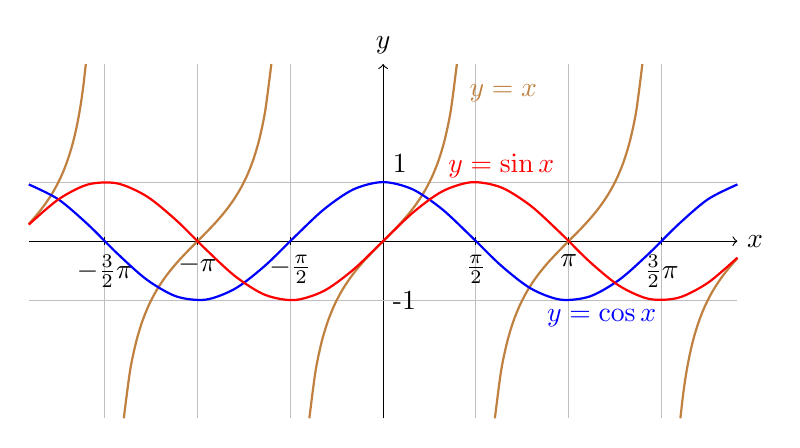
\begin{tikzpicture}[scale=0.75]
  \draw[->] (-6,0) -- (6,0) node[right] {$x$};
  \draw[->] (0,-3) -- (0,3) node[above] {$y$};
  \foreach \x/\xtext in
    {{pi/2}/{\frac \pi 2}, {pi}/{\pi}, {3*pi/2}/{\frac{3}{2}\pi},
    {-pi/2}/{-\frac \pi 2}, {-pi}/{-\pi}, {-3*pi/2}/{-\frac{3}{2}\pi}} {
    \draw[shift={(\x,0)},lightgray] (0,-3) -- (0,3);
    \draw[shift={(\x,0)}] (0pt,2pt) -- (0pt,-2pt) node[below] {$\xtext$};
  }
  \foreach \y in {1, -1} {
    \draw[shift={(0,\y)},lightgray] (-6,0) -- (6,0);
  }
  \draw (0,1) node [above right] {1};
  \draw (0,-1) node [right] {-1};
  \draw[domain=-rad(atan(3)):rad(atan(3)),smooth,variable=\x,brown,thick] plot ({\x},{tan(deg(\x))});
  \draw[domain=pi-rad(atan(3)):pi+rad(atan(3)),smooth,variable=\x,brown,thick] plot ({\x},{tan(deg(\x))});
  \draw[domain=-pi-rad(atan(3)):-pi+rad(atan(3)),smooth,variable=\x,brown,thick] plot ({\x},{tan(deg(\x))});
  \draw[domain=-6:-2*pi+rad(atan(3)),smooth,variable=\x,brown,thick] plot ({\x},{tan(deg(\x))});
  \draw[domain=2*pi-rad(atan(3)):6,smooth,variable=\x,brown,thick] plot ({\x},{tan(deg(\x))});
  \draw[domain=-6:6,smooth,variable=\x,blue,thick] plot ({\x},{cos(deg(\x))});
  \draw[domain=-6:6,smooth,variable=\x,red,thick] plot ({\x},{sin(deg(\x))});
  \draw (3.7,-1) node[blue,below] {$y=\cos x$};
  \draw (2,0.9)  node[red,above] {$y=\sin x$};
  \draw (1.3,2.5) node[brown,right] {$y=\tg x$};
  \end{tikzpicture}
  \caption{%
  I grafici delle funzioni $\sin$, $\cos$ e $\tg$.
  \ifwidemargin\\\\\fi%
  \usebox{\qrfigtrigo}}
\end{figure}

\subsection{funzioni trigonometriche inverse}

La funzione $\sin\colon[-\pi/2,\pi/2]\to [-1,1]$ 
risulta essere strettamente crescente e bigettiva. 
Dunque restringendo il dominio all'intervallo $[-\pi/2, \pi/2]$
e il codominio all'intervallo $[-1,1]$ la funzione risulta invertibile.
La funzione inversa
\[
  \arcsin\colon[-1,1]\to [-\pi/2, \pi/2]
\]
si chiama \emph{arco seno}. 
Per definizione di funzione inversa si ha
\[
  \arcsin(\sin x) = x, \qquad \forall x \in [-\pi/2, \pi/2]
\]
e
\[
  \sin(\arcsin x) = x, \qquad \forall x \in [-1, 1].
\]

La funzione $\cos \colon[0,\pi] \to [-1,1]$ risulta essere strettamente
decrescente e bigettiva.
La funzione inversa
\[
  \arccos\colon[-1,1] \to [0,\pi]
\]
si chiama \emph{arco coseno}. Per definizione si ha
\[
  \arccos(\cos x) = x, \qquad \forall x \in [0,\pi]
\]
e
\[
    \cos(\arccos x) = x, \qquad \forall x \in [-1,1].
\]

La funzione
\index{tangente!funzione trigonometrica}
\mymargin{$\tg x$}%
\index{$\tg x$}
\[
\tg x = \frac{\sin x}{\cos x}
\]
è definita quando $\cos x\neq 0$ ovvero:
\[
  \tg \colon \RR \setminus\ENCLOSE{\frac \pi 2+ k\pi\colon k\in \ZZ} \to \RR.
\]
Se restringiamo la funzione all'intervallo $\enclose{-\pi/2, \pi/2}$ possiamo
facilmente osservare che la funzione $\tg\colon(-\pi/2,\pi/2)\to \RR$ è strettamente crescente. Inoltre se $a_n \to \pi/2$, $a_n<\pi/2$ si ha $\cos(a_n)\to 0$ (per continuità del coseno) e $\sin(a_n)\to 1$ dunque $\tg a_n\to +\infty$. Analogamente per $a_n \to -\pi/2$ si trova $\tg a_n \to -\infty$. Dunque per il teorema dei valori intermedi possiamo affermare che la funzione $\tg\colon(-\pi/2,\pi/2)\to \RR$ è suriettiva. E' quindi invertibile
e la funzione inversa
\[
  \arctg \colon \RR \to (-\pi/2,\pi/2)
\]
si chiama \emph{arco tangente}. Per definizione si ha
\[
  \arctg \tg x = x, \qquad \forall x \in (-\pi/2, \pi/2)
\]
e
\[
  \tg\arctg x = x, \qquad \forall x \in \RR.
\]

Grazie al teorema~\ref{th:monotona_continua}
visto che queste funzioni sono monotone e bigettive
possiamo affermare che
le funzioni $\arcsin$, $\arccos$ e $\arctg$ 
sono tutte funzioni continue.

\begin{exercise}[funzioni misteriose]
  Si disegni il grafico delle seguenti funzioni
  \[
    f(x) = \arcsin \sin x, \qquad 
    g(x) = \arccos \cos x, \qquad 
    h(x) = \arctg \tg x.
  \]
  Si osservi che:
  \begin{enumerate} 
    \item $f$ e $g$ sono definite su tutto $\RR$,
  mentre $h$ è definita su $\RR\setminus\ENCLOSE{\frac{\pi}2+k\pi\colon k\in \ZZ}$;
    \item $f$ e $h$ hanno valori 
  in $\closeinterval{-\frac \pi 2}{\frac \pi 2}$
  mentre $g$ ha valori in $\closeinterval{0}{\pi}$;
    \item $f$ e $g$ hanno periodo $2\pi$,
  $h$ ha periodo $\pi$;
    \item tutte e tre sono funzioni continue (sul loro dominio).
  \end{enumerate}
\end{exercise}

\begin{exercise}
Dimostrare che per ogni $x>0$ si ha
\[
  \arctg \frac 1 x = \frac \pi 2 - \arctg x.
\]
\end{exercise}

\begin{exercise}[lunghezza della circonferenza]
Si osservi che un $n$-agono regolare iscritto a una circonferenza 
di raggio $r$ ha lati di lunghezza $l_n = 2r\sin \frac{\pi}{n}$
e quindi perimetro $p_n = n\cdot l_n$.
Si verifichi che 
\[
  \lim_{n\to +\infty} p_n = 2\pi r.
\]
\end{exercise}

\section{funzioni iperboliche}

\begin{definition}[funzioni iperboliche]
Le funzioni
\emph{coseno iperbolico} e \emph{seno iperbolico}
sono definite, per ogni $x\in \RR$,
come segue:
\mymargin{$\sinh$, $\cosh$}%
\index{$\sinh$, $\cosh$}%
\index{funzioni!iperboliche}%
\index{seno!iperbolico}%
\index{coseno!iperbolico}%
\index{$\sinh$}%
\index{$\cosh$}%
\begin{equation}
\label{eq:sinh_cosh}
  \cosh x = \frac{e^x + e^{-x}}{2},
  \qquad
  \sinh x = \frac{e^x - e^{-x}}{2}.
\end{equation}
\end{definition}

\begin{theorem}[proprietà delle funzioni iperboliche]
Valgono le seguenti proprietà.
\begin{enumerate}
\item
la funzione $\sinh$ è dispari, $\cosh$ è pari:
\[
\sinh(-x) = -\sinh(x),
\qquad
\cosh(-x) = \cosh(x);
\]

\item
i punti del piano con coordinate $(\cosh x, \sinh x)$
per $x\in \RR$
sono disposti su un ramo di iperbole in quanto vale:
\[
  \cosh^2 x - \sinh^2 x = 1;
\]

\item formule di addizione:
\begin{align*}
  \cosh(\alpha+\beta) &= \cosh \alpha \cosh \beta + \sinh \alpha \sinh \beta,\\
  \sinh(\alpha+\beta) &= \sinh \alpha \cosh \beta + \cosh \alpha \sinh \beta;
\end{align*}

% \item si ha
% \begin{align*}
%   \cosh x
%   &= \sum_{k=0}^{+\infty} \frac{x^{2k}}{(2k)!}
%   = 1 + \frac{x^2}{2} + \frac{x^4}{4!} + \frac{x^6}{6!} + \dots \\
%   \sinh x
%   &= \sum_{k=0}^{+\infty} \frac{x^{2k+1}}{(2k+1)!}
%   = x + \frac{x^3}{6} + \frac{x^5}{5!} + \frac{x^7}{7!} + \dots
% \end{align*}

\item
la funzione $\sinh$ è strettamente crescente su tutto $\RR$,
la funzione $\cosh$
è strettamente crescente sull'intervallo
$[0,+\infty)$ e strettamente decrescente
nell'intervallo $(-\infty,0]$;

\item per $x\to +\infty$ si ha $\sinh x \to +\infty$, $\cosh x \to +\infty$, 
per $x\to -\infty$ si ha $\sinh x \to -\infty$, $\cosh x \to +\infty$.

\end{enumerate}
\end{theorem}

\newsavebox{\qrfigiperb}\sbox{\qrfigiperb}{\myurlhere{figiperb}{funzioni iperboliche}}%
\begin{figure}
  \centering%
  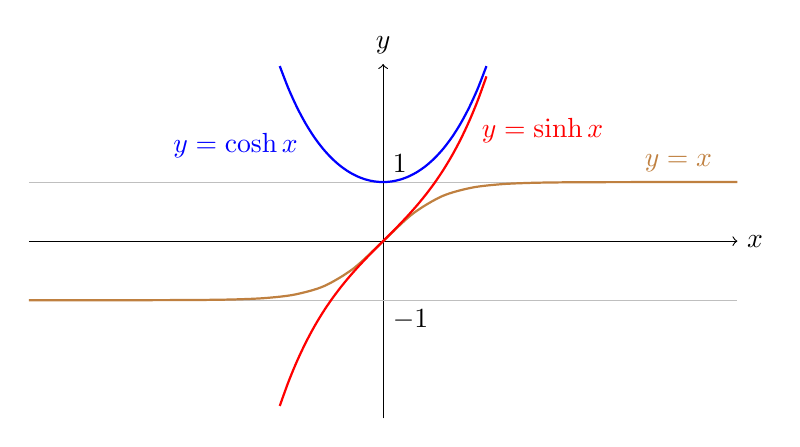
\begin{tikzpicture}[scale=0.75]
  \draw[->] (-6,0) -- (6,0) node[right] {$x$};
  \draw[->] (0,-3) -- (0,3) node[above] {$y$};
  \foreach \y in {1, -1} {
    \draw[shift={(0,\y)},lightgray] (-6,0) -- (6,0);
  }
  \draw (0,1) node [above right] {$1$};
  \draw (0,-1) node [below right] {$-1$};
  \draw[domain=-6:6,smooth,variable=\x,brown,thick] plot ({\x},{tanh(\x)});
  \draw[domain=-1.75:1.75,smooth,variable=\x,blue,thick] plot ({\x},{cosh(\x)});
  \draw[domain=-1.75:1.75,smooth,variable=\x,red,thick] plot ({\x},{sinh(\x)});
  \draw (-2.5,2) node[blue,below] {$y=\cosh x$};
  \draw (2.7,1.5)  node[red,above] {$y=\sinh x$};
  \draw (5,1) node[brown,above] {$y=\tgh x$};
  \end{tikzpicture}
  \caption{%
    I grafici delle funzioni $\sinh$, $\cosh$ e $\tgh$.
    \ifwidemargin\\\\\fi%
    \usebox{\qrfigiperb}%
  }
\end{figure}

\begin{proof}
I primi tre punti si dimostrano facilmente per verifica diretta,
utilizzando la definizione~\eqref{eq:sinh_cosh}.

% Gli sviluppi in serie si ottengono anch'essi sostituendo
% gli sviluppi dell'esponenziale nella definizione.
% Nel $\cosh$ i termini di grado dispari si cancellano, nel $\sinh$ si cancellano
% i termini di grado pari.

Per quanto riguarda la monotonia si osserva che se $x\ge 0$ ogni
addendo delle due serie esposte nel punto 4 è strettamente crescente
(in quanto i coefficienti sono tutti positivi) e dunque le somme delle serie,
cioè la funzione $\cosh$ e la funzione $\sinh$ sono strettamente crescenti
sull'intervallo $[0,+\infty)$. La funzione $\sinh$, essendo dispari,
risulta inoltre crescente anche sull'intervallo $(-\infty,0]$ e quindi
è crescente su tutto $\RR$.

Per l'ultima proprietà basterà usare la definizione~\eqref{eq:sinh_cosh}
e ricordare che (teorema~\ref{th:ordine_infinito})
se $x\to +\infty$ allora
$e^x\to +\infty$ ed $e^{-x}=\frac{1}{e^{x}} \to 0$.
\end{proof}

Osserviamo che $\cosh 0 = 1$ e, per le proprietà di monotonia viste nel teorema
precedente si ha $\cosh x \ge \cosh 0 = 1 > 0$. Dunque $\cosh x$ non si annulla
mai e si può definire per ogni $x\in \RR$ la \emph{tangente iperbolica}
\index{tangente!iperbolica}%
\mymargin{$\tgh$}%
\index{$\tgh$}%
\[
    \tgh x = \frac{\sinh x}{\cosh x}.
\]

La funzione $\sinh\colon \RR\to\RR$ è iniettiva in quanto strettamente crescente ed
è surgettiva in quanto è continua e quindi assume tutti i valori compresi tra
$\lim_{x\to+\infty} \sinh(x) = +\infty$ e $\lim_{x\to -\infty} \sinh(x) = -\infty$. 
Dunque $\sinh\colon \RR \to \RR$
è invertibile e la funzione inversa si chiama \emph{settore di seno iperbolico}
e si denota con
\mymargin{$\settsinh$}%
\index{$\settsinh$}
\index{settore!di seno iperbolico}
\[
    \settsinh \colon \RR \to \RR.
\]
Analogamente la funzione ristretta $\cosh\colon [0,+\infty)\to [1,+\infty)$ è
iniettiva in quanto strettamente crescente ed è surgettiva in quanto
è continua e assume su $[0,+\infty)$ tutti i valori compresi tra $\cosh(0)=1$ e
$\lim_{x\to +\infty} \cosh x = +\infty$.
Dunque la funzione $\cosh x$ ristretta a $[0,+\infty)\to [1,+\infty)$
è invertibile e la funzione inversa si chiama \emph{settore di coseno iperbolico}
\mymargin{$\settcosh$}%
\index{$\settcosh$}
\index{settore!di coseno iperbolico}
\[
    \settcosh \colon [1,+\infty)\to [0,+\infty).
\]

La funzione $\tgh x$ è strettamente crescente su tutto $\RR$ e assume tutti i valori strettamente compresi tra $-1$ e $1$.
La funzione inversa si chiama $\setttgh$.

\begin{exercise}
Fissato $y\in \RR$ si risolva l'equazione
\[
    \frac{e^x - e^{-x}}{2} = y
\]
riconducendola ad una equazione di secondo grado nella variabile $t=e^x$.
Si dimostri quindi che vale
\[
    \settsinh x = \ln\enclose{x + \sqrt{x^2 + 1}}.
\]
In modo analogo si dimostri che vale
\[
    \settcosh x = \ln\enclose{x + \sqrt{x^2 - 1}}
\]
e
\[
    \setttgh x = \ln \sqrt{\frac{1+x}{1-x}}.
\]
\end{exercise}

\section{l'esponenziale complesso}
\label{sec:esponenziale_complesso}%

L'esponenziale reale e le funzioni trigonometriche possono essere pensate 
come strumenti intermedi per definire un isomorfismo naturale 
da $\CC$ come gruppo additivo in $\CC$ come gruppo moltiplicativo.

Possiamo infatti definire la funzione $\exp \colon \CC \to \CC$ mediante 
la \emph{formula di Eulero}
\[
 \exp(x+iy) = e^x \cdot (\cos y + i \sin y).
\]
Questa funzione ha le seguenti proprietà:
\begin{enumerate}
  \item $\exp(z+w) = \exp z \cdot \exp w$;
  \item $\exp\bar z = \overline{\exp z}$;
  \item $\abs{\exp z} = e^{\Re z}$;
  \item $\exp x = e^x$ se $x\in \RR$.
\end{enumerate}
Visto che $\exp$ estende la funzione esponenziale reale $e^x$
sarà anche naturale usare la stessa notazione ponendo:
\mynote{%
La notazione $e^z$ non ci deve far pensare che abbiamo definito 
una operazione di elevamento a potenza tra numeri complessi. 
In effetti non è possibile definire in maniera sensata e univoca 
la potenza $z^w$ se la base $z$ non è un numero reale positivo.
Questo è legato al fatto che la funzione esponenziale $e^z$
non è univocamente invertibile e quindi non si può definire il 
logaritmo $\ln z$ se non come funzione \emph{multivoca}.
}%
\[
  e^z = \exp z = e^x\cdot (\cos y + i\sin y), \qquad \text{se $z=x+iy$}.  
\]

Si noti che la funzione esponenziale complessa è $2\pi i$ periodica, infatti 
se $z=x+iy$ si ha 
\[
\exp(z+2\pi i) 
= e^x\cdot (\cos(y+2\pi) + i\sin(y+2\pi)) 
= e^x\cdot (\cos y + i \sin y) 
= \exp(z).
\]

% Nel capitolo precedente abbiamo introdotto l'esponenziale complesso ed
% abbiamo osservato che la funzione $f\colon \RR \to \CC$ definita da
% $f(t) = e^{it}$ ha valori sulla circonferenza unitaria in quanto
% $\abs{e^{it}}=1$. Tramite la definizione~\ref{def:sincos}
% abbiamo introdotto le funzioni seno e coseno in
% modo che risulti $f(t) = \cos t + i \sin t$.
% Sappiamo che $f(0) = e^0 = 1$ e, per come abbiamo definito $\pi$,
% sappiamo che $f(\pi/2) = i$.

\subsection{rappresentazione polare dei numeri complessi}

Per come li abbiamo definiti i numeri complessi $z\in \CC$ si possono 
rappresentare nella forma:
\[
  z = x + i y.
\]
Questa rappresentazione dei numeri complessi viene chiamata \emph{cartesiana}
perché fa corrispondere ogni numero $z$ alle sue coordinate $(x,y)$ nel
piano complesso (piano di Gauss). 

Grazie alla definizione di esponenziale complesso possiamo anche 
dare una rappresentazione \emph{polare} dei numeri complessi.
Se $z=x+iy$ è un qualunque numero complesso possiamo definire 
$\rho = \abs{z} = \sqrt{x^2+y^2}$ il suo \emph{modulo} 
ovvero la distanza geometrica tra il punto $z$ del piano complesso 
e l'origine $0\in \CC$.
Se $z\neq 0$ possiamo definire la misura dell'angolo individuato 
da $z$ con l'asse delle $x$ come quell'unico 
$\theta \in \closeopeninterval{0}{2\pi}$ tale che
\[
  \begin{cases}
    x = \rho \cos \theta,\\
    y = \rho \sin \theta.
  \end{cases}
\]
Si ha quindi 
\[
  z = \rho \cdot (\cos \theta + i \sin \theta). 
\]
La coppia di numeri $(\theta,\rho)$ con $\rho>0$ e $\theta\in\closeopeninterval{0}{2\pi}$ 
si chiamano \emph{coordinate polari} del numero complesso $z$ 
e identificano univocamente $z$. 
Per la periodicità delle funzioni $\sin$ e $\cos$ risulta chiaro 
che l'angolo $\theta$ può essere sostitutito con $\theta +2k\pi$ 
per qualunque $k\in \ZZ$ lasciando invariato il punto $z$.
Se $z=0$ allora $\rho=\abs{z}=0$ e la coordinata $\theta$ è irrilevante.

La rappresentazione \emph{esponenziale} di un numero complesso 
è sostanzialmente identica alla rappresentazione polare 
ma utilizza l'esponenziale complesso invece che 
le funzioni trigonometriche. 
Essendo $e^{i\theta} = \cos \theta + i\sin \theta$
se $z=\rho\cdot (\cos \theta + i \sin \theta)$ potremo scrivere:
\[
  z = \rho \cdot e^{i\theta}.  
\]

Se $z=\rho e^{i\theta}$
il numero $\theta$ viene usualmente chiamato \emph{argomento}
del numero complesso $z$ e si denota a volte 
in questo modo:
\[
  \theta = \arg z.  
\]
La definizione di argomento è intrinsecamente ambigua 
in quanto $\theta$ non è univocamente determinato
(al posto di $\theta$ possiamo scegliere $\theta+2k\pi)$ 
con qualunque $k\in \ZZ$).
Per avere una definizione univoca si può imporre 
la condizione $\theta\in\closeopeninterval{0}{2\pi}$.
\mynote{Ma la condizione 
$\theta\in\closeinterval{-\pi}{\pi}$ 
andrebbe ugualmente bene.}
Se $z=0$ possiamo definire, arbitrariamente, 
$\arg z = 0$. 
In formule si ha:
\[
  \arg z =
  \begin{cases}
%   \arctg \frac y x & \text{se $x>0$,} \\
   \frac \pi 2 - \arctg \frac x y & \text{se $y>0$,} \\
   \frac 3 2 \pi- \arctg \frac x y & \text{se $y<0$,} \\
   \pi & \text{se $y=0$ e $x<0$,} \\
   0 & \text{se $y=0$ e $x\ge 0$.}
   \end{cases}
\]

\subsection{radici complesse $n$-esime}

Sia $c\in \CC$ un numero
complesso $c\neq 0$.
Ci poniamo il problema di determinare le soluzioni complesse
dell'equazione
\[
  z^n = c.
\]
Tali soluzioni saranno chiamate \emph{radici $n$-esime}%
\mymargin{radici $n$-esime}%
\index{radice!$n$-esima} di $c$.

Scriviamo $c$ e $z$ in forma esponenziale:
\[
  c = r e^{i\alpha}, \qquad
  z = \rho e^{i\theta}.
\]
Si avrà allora
\[
  z^n = \rho^n (e^{i\theta})^n = \rho^n e^{i n \theta}.
\]
Affinche sia $z^n = c$ si dovrà avere l'uguaglianza dei moduli, cioè $\rho^n = r$ e l'uguaglianza a meno di multipli interi di $2\pi$ degli argomenti:
$n \theta = \alpha + 2 k \pi$ con $k\in \ZZ$.
Dunque si trova
\[
  \theta = \frac{\alpha}{n} + k\frac{2\pi}{n}
\qquad k \in \ZZ.
\]
Osserviamo ora che per $k=0,\dots, n-1$ il secondo addendo
$k 2\pi /n$ assume $n$ valori distinti compresi in $[0,2\pi)$.
Per gli altri valori di $k$ si ottengono degli angoli che differiscono
da questi di un multiplo di $2\pi$ e quindi non si trovano
altre soluzioni.

Dunque l'equazione $z^n = c$ per $c\neq 0$ ha $n$ soluzioni distinte date
da
\[
z_k = \sqrt[n]{r} \cdot e^{i\alpha/n + 2k\pi i /n},
\qquad k=0,1, \dots, n-1
\]
dove $\alpha = \arg(c)$ e $r = \abs{c}$.
Dal punto di vista geometrico si osserva che
$z_0$ è il numero complesso con modulo la radice $n$-esima del numero
dato $c$ e argomento pari ad un $n$-esimo dell'argomento di $c$.
Tutte le altre soluzioni si trovano sulla circonferenza centrata in $0$
e passante per $z_0$ e risultano essere, insieme ad $z_0$, i vertici
di un $n$-agono regolare.

In particolare nel caso $c=1$ si osserva che le radici $n$-esime dell'unità
si rappresentano geometricamente come i vertici dell'$n$-agono regolare iscritto
nella circonferenza unitaria e con un vertice in $z_0=1$.

\begin{exercise}
Si trovino le soluzioni $z \in \CC$ delle seguenti equazioni.
Scrivere le soluzioni in forma polare e cartesiana.
\begin{gather*}
   z^4 = -4 \\
   z^6 = i\\
   z^3 = -8i \\
   z^4 = z\\
   z^2 + 1 = i\sqrt{3} \\
   (z-i)^4 = 1\\
   1 + z + z^2 + z^3 = 0\\
   z^{14} - z^6 - z^8 + 1 = 0
\end{gather*}
\end{exercise}

\section{polinomi complessi}
\label{ch:ancora_polinomi}

\subsection{il teorema fondamentale dell'algebra}

Il teorema fondamentale dell'algebra afferma che ogni polinomio non costante 
si annulla in almeno un punto del piano complesso.
\mynote{si vedano le note storiche a fine capitolo}
Per dimostrare il teorema dobbiamo estendere il teorema 
di Weierstrass alle funzioni di una variabile complessa.
Nel teorema di Weierstrass reale la funzione per ipotesi è definita su un intervallo
chiuso e limitato. 
Nel piano complesso non esiste il concetto di \emph{intervallo} in quanto non abbiamo 
un ordinamento ma vedremo che comunque il teorema di Weierstrass rimane valido per 
le funzioni continue definite su insiemi chiusi e limitati secondo le seguenti definizioni.

\begin{definition}[chiusura sequenziale]
Un insieme $A\subset \CC$ si dice
essere \emph{sequenzialmente chiuso}
\mymargin{sequenzialmente chiuso}%
\index{sequenzialmente!chiuso}%
se presa una qualunque successione
di punti $a_n\in A$ se $a_n \to a$ per qualche $a\in \CC$
allora $a\in A$.
\end{definition}

\begin{definition}[limitatezza]
Un insieme $A\subset \CC$ si dice essere \emph{limitato}%
\mymargin{limitato}%
\index{limitato}
se
\[
  \sup \ENCLOSE{ \abs{z}\colon z \in A} < +\infty.
\]
\end{definition}

Si noti che una successione $a_n\in \CC$ 
è limitata (si veda capitolo~\ref{sec:successione_limitata})
se e solo se la sua immagine $\ENCLOSE{a_n\colon n\in \NN}\subset \CC$
è un insieme limitato.

% \begin{theorem}[Bolzano-Weierstrass complesso]
% Se $z_n\in \CC$ è una successione limitata allora
% è possibile estrarre una sottosuccessione $z_{n_k}$ convergente:
% $z_{n_k} \to z$ con $z\in \CC$.
% \end{theorem}
% %
% \begin{proof}
% Siano $x_n$ e $y_n$ la parte reale ed immaginaria di $z_n$: $z_n = x_n + i y_n$. Visto che $\abs{x_n} =\sqrt{x_n^2}\le \sqrt{x_n^2+y_n^2} = \abs{z_n}$ e, allo stesso modo $\abs{y_n} \le \abs{z_n}$,
% possiamo affermare che entrambe le successioni $x_n$ e $y_n$ sono limitate (ma stavolta in $\RR$).
% Dunque possiamo applicare il teorema di Bolzano-Weierstrass (reale) alla successione $x_n$ per trovare una sottosuccessione $x_{n_j}\to x$ convergente. E possiamo applicare di nuovo il teorema di Bolzano-Weierstrass alla sottosuccessione $y_{n_j}$ per trovare una sotto-sottosuccessione $y_{n_{j_k}}\to y$ anch'essa convergente.
% Posto $n_k = n_{j_k}$ avremo dunque trovato una sottosuccessione $z_{n_k} = x_{n_k} + i y_{n_k} \to x+iy$ convergente.
% \end{proof}

\begin{theorem}[Weierstrass complesso]
Sia $A\subset \CC$ un insieme non vuoto, sequenzialmente chiuso e limitato e sia $f\colon A \to \RR$ una funzione continua.
Allora $f$ ha massimo e minimo su $A$.
\end{theorem}
%
\begin{proof}
Dimostriamo l'esistenza del minimo: per il massimo la dimostrazione è perfettamente analoga.
Sia $m=\inf f(A)$.
Essendo $A$ non vuoto, per il lemma sull'esistenza delle successioni minimizzanti sappiamo esistere una successione $z_n \in A$ tale che $f(z_n) \to m$.
Essendo $A$ limitato possiamo applicare il teorema di Bolzano-Weierstrass per trovare $z\in \CC$ e una sottosuccessione $z_{n_k} \to z$. Essendo $A$ sequenzialmente chiuso possiamo quindi affermare che $z\in A$. Essendo $f$ continua concludiamo che
\[
f(z) = \lim_{k\to+\infty} f(z_{n_k}) = m
\]
e dunque $z$ è un punto di minimo per $f$.
\end{proof}

\begin{theorem}[esistenza del minimo per funzioni coercive]
Sia $f\colon \CC \to \RR$ una funzione continua tale che per ogni
successione $z_n \to \infty$ (ovvero $\abs{z_n}\to +\infty$)
si abbia $f(z_n) \to +\infty$.
Allora $f$ ha minimo.
\end{theorem}
%
\begin{proof}
Consideriamo l'insieme
\[
  A = \ENCLOSE{z \in \CC \colon f(z) \le f(0)}.
\]
Chiaramente $0\in A$ e quindi $A$ non è vuoto.
L'insieme $A$ è anche sequenzialmente chiuso in quanto se $z_k\in A$ allora $f(0) - f(z_k)\ge 0$,
per continuità $f(0)-f(z_k)\to f(0)-f(z)$
e per il teorema della permanenza del segno si ottiene $f(0)-f(z) \ge 0$ cioè $z \in A$.
Dimostriamo ora che $A$ è anche limitato. 
Se non lo fosse esisterebbe, per assurdo, una successione $z_n \in A$ tale che $\abs{z_n}\to +\infty$ cioè $z_n \to \infty$. 
Ma allora, per ipotesi su $f$, si avrebbe $f(z_n)\to +\infty$ che contraddice la condizione $f(z_n) \le f(0)$. 
Essendo $A$ non vuoto, sequenzialmente chiuso e limitato ed essendo $f\colon A \to \RR$ continua, 
possiamo applicare il teorema di Weierstrass complesso per dedurre che $f$ ha minimo su $A$ in un punto $w \in A$. 
Ma essendo $0\in A$ si avrà sicuramente $f(w)\le f(0)$ e per ogni $z\in \CC \setminus A$ si ha invece $f(z) > f(0)$ per come è stato definito $A$. 
Dunque $w$ è minimo di $f$ su tutto $\CC$, non solo su $A$.
\end{proof}

\begin{theorem}[teorema fondamentale dell'algebra]
\label{th:fondamentale_algebra}
\mymargin{teorema fondamentale dell'algebra}%
\index{teorema!fondamentale dell'algebra}%
Sia $f(z)$ un polinomio di grado $N\ge 1$ a coefficienti complessi:
\[
  f(z) = \sum_{j=0}^N a_j \cdot z^j
\]
con $a_j\in \CC$ per $j=0,\dots,N$ e $a_N \neq 0$.
Allora esiste $w\in \CC$ tale che $f(w) = 0$.
\end{theorem}
%
\begin{proof}
  Osserviamo innanzitutto che $\abs{f(z)}$ è coerciva cioè che
  se $z_n \to \infty$ allora $\abs{f(z_n)}\to +\infty$.
  Infatti si ha
  \begin{align*}
    \abs{f(z_n)}
    &= \abs{\sum_{j=0}^N a_j z_n^j}
    = \abs{a_N z_n^N  + \sum_{j=0}^{N-1} a_j z_n^j}\\
    &= \abs{z_n}^N \cdot \abs{a_N + \sum_{j=0}^{N-1} \frac{a_j}{z_n^{N-j}}}
    \to +\infty
  \end{align*}
  se $z_n \to \infty$.
  
  Sappiamo che tutti i polinomi sono funzioni continue in quanto somme di 
  prodotti di funzioni continue e il modulo è anch'esso una funzione continua 
  dunque $\abs{f(z)}$ è certamente una funzione continua.
  
  Dunque possiamo applicare il teorema di esistenza del minimo per le funzioni 
  coercive: esiste $w\in \CC$ tale che $\abs{f(w)}$ è minimo.
  
  Per concludere il teorema basterà dimostrare che $f(w)=0$.
  L'idea che vogliamo sviluppare è che i polinomi complessi se assumono un valore
  $f(w)$ in un punto $w\in \CC$ allora assumono anche tutti i valori vicini
  ad esso in quanto \emph{localmente} il polinomio assomiglia ad una potenza $z^n$
  e l'equazione $z^n=c$ ha sempre soluzione, come abbiamo già visto.
  Dunque vicino a $w$ ci saranno dei punti in cui $f$ assume valori che in modulo 
  sono minori a $f(w)$: a meno che non sia proprio $f(w)=0$, nel qual caso 
  ovviamente non è possibile avere numeri con modulo inferiore a $0$.
  
  Possiamo scrivere il polinomio $f(z)$ nella forma
  \[
    f(z) = \sum_{j=0}^N b_j (z-w)^j
  \]
  in quanto la traslazione di un polinomio è ancora un polinomio dello stesso 
  grado.
  Dimostrare che $f(w)=0$ è quindi equivalente a dimostrare che $b_0=0$.
  Supponiamo allora per assurdo che sia $b_0\neq 0$. 
  L'andamento del polinomio vicino al punto $w$ è dominato dai termini di grado 
  più basso: alcuni di questi potrebbero essere nulli, ma possiamo considerare 
  il primo indice $k>0$ per cui si ha $b_k\neq 0$. Allora potremo scrivere:
  \[
      f(z) = b_0 + b_k(z-w)^k + \sum_{j=k+1}^N b_j (z-w)^j.
  \]
Ora scriviamo $z-w$, $b_0$ e $b_k$ in forma esponenziale:
$z - w = \rho e^{i\theta}$, $b_0 = r_0 e^{i \alpha_0}$,
$b_k = r_k e^{i\alpha_k}$ 
e applichiamo la disuguaglianza triangolare
  \begin{align*}
    \abs{f(z)} 
    &= \abs{r e^{i\alpha} + r_k \rho^k e^{i(\theta k+\alpha_k)} 
    + \sum_{j=k+1}^N b_j \rho^j e^{i\theta j}} \\
    &\le \abs{r e^{i\alpha} + r_k \rho^k e^{i(\theta k + \alpha_k )}} 
    + \sum_{j=k+1}^N \abs{b_j} \rho^j.
  \end{align*}
Per raggiungere un assurdo vogliamo dimostrare che esiste $z$ (cioè esistono $\rho$ e $\theta$)
per cui il valore della funzione risulti in modulo minore di $r = \abs{b_0} = \abs{f(w)}$.
Innanzitutto se $\rho$ è sufficientemente piccolo possiamo rendere arbitrariamente piccole 
le potenze $\rho^j$ con $\rho>k$: basta scegliere $\rho\le 1$ 
e $\rho \le r_k/(2\sum \abs{b_j})$
cosicché si avrà 
\[
  \sum_{j=k+1}^N \abs{b_j} \rho^j
  \le \rho^{k+1} \sum_{j=k+1}^N \abs{b_j} \le r_k\frac{\rho^{k}}{2}.
\]
Per quanto riguarda il termine
$r e^{i\alpha} + r_k \rho^k e^{i(\theta k + \alpha_k)}$ 
sarà sufficiente scegliere $\theta = (\pi + \alpha - \alpha_k) /k$ 
in modo che i due addendi 
abbiano fase opposta e la somma sia distruttiva:
\[
  \abs{r e^{i\alpha} + r_k \rho^k e^{i(\theta k + \alpha_k)}}
  = \abs{e^{i\alpha}(r + r_k \rho^k e^{i\pi})}
  = r - r_k\rho^k.
\]
In definitiva abbiamo
\[
\abs{f(z)} = \abs{f(w+\rho e^{i\theta}} 
\le r - r_k\rho^k + r_k\frac{\rho^k}{2} 
< r = \abs{f(w)}
\]
che è assurdo in quanto $\abs{f(w)}$ doveva essere il valore minimo.
\end{proof}
  
\subsection{fattorizzazione dei polinomi}

\begin{theorem}[fattorizzazione dei polinomi complessi]
\index{decomposizione!dei polinomi complessi}%
\index{fattorizzazione!dei polinomi complessi}%
\index{polinomio!fattorizzazione complessa}%
Sia $p(z)$ un polinomio non nullo. Allora posto $n=\deg p$ esistono dei numeri complessi $z_1, z_2, \dots, z_n$ ed un numero complesso $c\neq 0$ tali che
\begin{equation}\label{eq:34985}
  p(z) = c \prod_{k=1}^n (z-z_k).
\end{equation}
Gli $z_k$ sono unici a meno dell'ordine e $c$ pure è univocamente determinato.
\end{theorem}
%
\begin{proof}
Dimostriamo il teorema per induzione su $n=\deg p$. Se $n=0$ il polinomio $p$ è costante: $p(z) = c$. Ricordando che un prodotto di $n=0$ fattori è uguale a $1$ si ottiene quindi il risultato voluto.

Sia ora $p(z)$ un qualunque polinomio di grado $n>0$. Per il teorema fondamentale dell'algebra sappiamo che esiste un numero complesso $z_n$ tale che $p(z_n)=0$. Per il teorema di Ruffini si ha allora
\[
  p(z) = (z-z_n) q(z)
\]
con $q$ un qualche polinomio di grado $n-1$. Per ipotesi induttiva possiamo dunque supporre che esistano $z_1, \dots, z_{n-1}$ e $c$ numeri complessi tali che
\[
   q(z) = c \prod_{k=1}^{n-1} (z-z_k)
\]
e la tesi segue.
\end{proof}

Nella fattorizzazione~\eqref{eq:34985} le \emph{radici} $z_k$ possono
anche ripetersi. Se mettiamo insieme i fattori corrispondenti alla stessa radice
si ottiene una decomposizione della forma
\begin{equation}\label{eq:358925}
P(z) = c \prod_{k=1}^m (z-z_k)^{p_k}
\end{equation}
con $z_1, \dots, z_m$ numeri complessi distinti (le radici del polinomio $P$)
e $p_k$ interi positivi.
L'esponente $p_k$ si chiama
\emph{molteplicità}%
\mymargin{molteplicità}%
\index{molteplicità} della radice $z_k$ e risulta
\[
  p_1 + \dots + p_m = n.
\]
Questa uguaglianza si esprime dicendo che un polinomio $P\in \CC[z]$
di grado $n$ ha sempre $n$ radici contate con la loro molteplicità.
Le radici distinte sono invece $m\le n$.

Se invece $P\in \RR[x]$ è un polinomio a coefficienti reali
non è detto che $P$ abbia radici: ad esempio il
polinomio $x^2+1$ non ha radici reali in quanto $x^2+1>0$
come succede in ogni campo ordinato.
Potrà allora essere utile pensare a $P$ come ad un polinomio
in $\CC[x]$ con coefficienti reali.

Se $P\in \RR[x]$ è un polinomio a coefficienti reali
\[
  P = \sum_{k=0}^n a_k x^k, \qquad a_k\in \RR
\]
possiamo pensare a $P$ anche come un polinomio in
$\CC[x]$, visto che $a_k\in \RR\subset \CC$.
Il seguente teorema ci dà un criterio per distinguere
i polinomi a coefficienti reali dentro a $\CC[x]$.

\begin{theorem}
\label{th:caratterizzazione_polinomi_reali}%
Se $P\in \CC[x]$ è un polinomio a coefficienti complessi
\[
  P = \sum_{k=0}^n a_k x^k,\qquad a_k\in \CC
\]
e se esiste un insieme infinito $A\subset \RR$
tale che per ogni $x\in A$ si abbia $P(x)\in \RR$
allora $a_k\in\RR$ per ogni $k=0,\dots,n$ e dunque $P\in \RR[x]$.

In particolare se la funzione polinomiale associata a
$P\in\CC[x]$ manda $\RR$ in $\RR$ allora $P$ è un polinomio
a coefficienti reali.
\end{theorem}
%
\begin{proof}
Consideriamo il polinomio:
\[
  Q = \sum_{k=0}^n (a_k-\bar a_k) x^k.
\]
Allora per ogni $x\in A$ si ha
\[
  Q(x) = \sum_{k=0}^n a_k x^k - \sum_{k=0}^n \bar a_k x^k
     = P(x) - \overline{P(x)} = P(x) - P(x) = 0
\]
in quanto se $x\in \RR$ risulta
$\overline{x^k} = {\bar x}^k = x^k$.
Visto che $A$ è infinito,
per il principio di annullamento dei polinomi
(teorema~\ref{th:annullamento_polinomi})
deduciamo che $Q=0$.
Ma allora tutti i coefficienti di $Q$ devono
essere nulli e cioè $\bar a_k = a_k$.
Ne consegue che $a_k\in \RR$ per ogni $k=0,\dots,n$.
\end{proof}

Rifacendoci alla fattorizzazione dei polinomi a coefficienti
complessi possiamo fattorizzare anche i polinomi a coefficienti
reali se ci accontentiamo di avere fattori quadratici
invece che lineari.

\begin{theorem}[fattorizzazione dei polinomi reali]
  \label{th:fattorizzazione_polinomio_reale}%
Se $P\in \RR[x]$ è un polinomio a coefficienti reali
potremo scrivere
\begin{equation}\label{eq:35549}
  P = a \cdot \prod_{k=1}^n (x-x_k)^{p_k} \cdot \prod_{j=1}^m (x^2 + \alpha_j x + \beta_j)^{q_j}
\end{equation}
dove $a\in \RR$, $x_k\in \RR$, $p_k\in \NN\setminus\ENCLOSE{0}$,
$\alpha_j,\beta_j\in \RR$, $q_j\in \NN\setminus\ENCLOSE{0}$
con $\alpha_j^2 - 4 \beta_j < 0$
e
\[
  \sum_{k=1}^n p_k + 2 \sum_{j=1}^m q_j = \deg P.
\]

La fattorizzazione~\eqref{eq:35549} è unica a meno
dell'ordine dei fattori.

I numeri $x_1,\dots,x_n$ sono tutte le radici reali distinte
del polinomio $P$ con rispettive molteplicità
$p_1,\dots,p_n$ mentre tutte le radici complesse (non reali)
distinte saranno $\mu_1,\dots, \mu_m$
e $\bar \mu_1, \dots, \bar \mu_m$ con
\[
  x^2 + \alpha_j x + \beta_j = (x-\mu)\cdot(x-\bar \mu)
\]
da cui
\[
  \alpha_j = -2\Re \mu_j, \qquad \beta_j=\abs{\mu_j}^2
\]
e $q_j$ saranno le molteplicità delle radici $\mu_j$
 e $\bar \mu_j$.
\end{theorem}
%
\begin{proof}
Osserviamo innanzitutto che se $P$ è a coefficienti reali
si ha
\[
  \overline{P(z)} = P(\bar z), \qquad \forall z\in \CC
\]
dunque se $\mu$ è una radice di $P$ anche $\bar \mu$
è una radice di $P$.
Ora se $\mu$ è una radice non reale di $P$ sappiamo
che in campo complesso $P$ risulta divisibile
per $x-\mu$ (teorema~\ref{th:Ruffini} di Ruffini):
\[
  P = (x-\mu) \cdot P_1.
\]
Ma anche $\bar \mu$ è radice di $P$ ed essendo
$\bar \mu \neq \mu$ si dovrà avere
\[
Q(\bar \mu) = \frac{P(\bar \mu)}{\bar \mu - \mu} = 0
\]
e dunque applicando nuovamente il teorema di Ruffini
\[
 P = (x-\mu)\cdot (x-\bar \mu)\cdot P_2.
\]
Ora osserviamo che
\[
(x-\mu)\cdot(x-\bar \mu) = x^2 - (\mu + \bar \mu) x + \mu \bar \mu
 = x^2 - 2 (\Re \mu)\cdot x + \abs{\mu}^2
\]
è un polinomio a coefficienti reali e
visto che $P_2$ si ottiene dividendo $P$ per tale polinomio,
anche $P_2$ è un polinomio a coefficienti reali.

Ripetendo lo stesso procedimento sul polinomio $P_2$
potremo fattorizzare $P$ diminuendo il grado a passi
di $2$ finché non si esauriscono tutte le radici complesse
non reali accoppiandole a due a due.
Dunque se $\mu$ è una radice complessa
del polinomio reale $P$ la molteplicità di $\mu$ è
uguale alla molteplicità di $\bar \mu$.

Dopodiché
si potrà completare la fattorizzazione dividendo
per i fattori lineari $x-x_k$ corrispondenti
alle radici reali del polinomio $P$.
Si otterrà quindi la fattorizzazione desiderata.
\end{proof}


\section{note storiche}

\subsection{il numero $e$}

\begin{figure}
  \begin{center}
  \includegraphics[width=10cm]{napier_tables.jpg}
  \end{center}
  \caption{Una pagina delle tavole calcolate da John Napier
  con i valori della funzione $\sin$ (Sinus) e del suo logaritmo
  (Logarithmi).
  In questa pagina ci sono i valori 
  per gli angoli dai 9 gradi (Gr.) ai 9 gradi e mezzo (i gradi 
  sessagesimali sono suddivisi in 60 minuti) e 
  dei loro complementari dagli 80 gradi e mezzo agli 81 gradi.
  Il codice scritto a pag.~\pageref{code:napier} permette
  di calcolare in pochi centesimi di secondo gli stessi valori
  mettendo anche in evidenza alcuni errori sulle ultime cifre decimali.
  Napier ci mise 20 anni a completare la stesura 
  delle tavole da 0 a 90 gradi.
  Se ad esempio volessimo calcolare il valore della tangente di $\alpha=9$ gradi 
  potremmo osservare che il logaritmo di $\tg \alpha$ 
  è la differenza tra il logaritmo di $\sin \alpha$ e il 
  logaritmo di $\cos \alpha$.
  Essendo il $\cos$ uguale al seno dell'angolo complementare 
  troviamo questo valore nella tabella in figura, 
  riga 0, colonna 
  \emph{Differenti\ae}: $1.8427293$ 
  (tutti i valori sono moltiplicati per $10^7$).
  Il valore cercato è l'esponenziale di questo 
  logaritmo e possiamo quindi calcolarlo cercando 
  lo stesso valore nella colonna \emph{Logarithmi}
  e prendendo il corrispondente valore nella colonna 
  \emph{Sinus}. Il valore è compreso tra i valori 
  della riga 6 e della riga 7. Più precisamente 
  differisce dal valore nella riga 7 
  $\frac{3842}{18143}$ volte quanto differisce il valore 
  della riga 6 dal valore della riga 7. 
  Applicando lo stesso rapporto ai valori trovati 
  nella colonna \emph{Sinus} si ottiene
  per interpolazione che al valore 
  della riga 7 (pari a 1.584453) và 
  sottratto 608 ottenendo quindi $\tg \alpha \approx 0.1583845$
  che differisce dal valore 
  esatto per meno di $10^{-7}$.
  }
  \label{fig:napier}
\end{figure}

\label{nota:Nepero}%
\index{Napier!John}%
\index{Nepero}%
\label{Euler!Leonhard}%
\label{Eulero}%
Nepero è l'italianizzazione del nome del
matematico scozzese \emph{John Napier} (1550-1617)
che per compilare le tavole della funzione seno
con una precisione di 7 cifre decimali ha introdotto 
per primo la funzione logaritmo (si veda la figura~\ref{fig:napier}).
E' interessante notare che Napier ha definito direttamente 
il logaritmo naturale senza introdurre il numero $e$ 
e senza fare alcun collegamento con la funzione esponenziale.
% https://archive.org/details/johnnapierinvent00hobsiala/page/18/mode/2up

\label{note:Bernoulli}%
\index{Bernoulli!Jacob}%
L'individuazione della costante $e$
è dovuta a \emph{Jacob Bernoulli} (1655--1705) nel 1683.
Bernoulli si chiedeva qual è l'interesse annuo effettivo
che si ottiene da un capitale che dia una rendita
giornaliera.
Se investo un capitale $c$ ad un tasso di interesse annuo 
pari a $r$, alla fine dell'anno mi viene restituito 
il capitale $c$ più un interesse $rc$.
Se divido il guadagno $rc$ per il numero di giorni che ci sono in 
un anno, posso considerare di aver avuto un guadagno giornaliero
pari a $\frac{r}{365} c$.
Se il guadagno giornaliero $\frac{r}{365} c$ mi venisse restituito 
immediatamente ogni giorno dell'anno, potrei reinvestire immediatamente 
il guadagno facendo aumentare il capitale durante l'anno.
In tal modo se parto con un capitale $c$ ogni giorno il mio capitale 
aumenterebbe di un fattore $1+\frac{r}{365}$ e
alla fine dell'anno avrei quindi un guadagno
pari a $\enclose{1+\frac{r}{365}}^{365} \approx e^r$ 
volte il capitale iniziale (interesse composto).

Il nome $e$ è stato introdotto da Eulero (Leonhard Euler 1707-1783).
%http://eulerarchive.maa.org//docs/originals/E853.pdf

\subsection{il teorema fondamentale dell'algebra}

La formula risolutiva per determinare le radici di un polinomio di secondo grado 
era già nota ai Babilonesi e sebbene i numeri complessi non erano noti 
(e neanche i numeri negativi) la stessa formula si applica 
nel caso generale e fornisce le radici complesse.

Lo studio delle equazioni di grado superiore al secondo si sviluppa invece 
nel 1500 ad opera dei matematici italiani Scipione del Ferro, 
Gerolamo Cardano, Niccolò Tartaglia e Lodovico Ferrari.
Essi determinano le formule risolutive per determinare le radici 
dei polinomi di terzo e quarto grado. 
Nell'applicare la formula risolutiva per l'equazione di terzo grado 
può capitare di dover calcolare la radice quadrata di un numero negativo
anche in situazioni in cui tutte le soluzioni alla fine risultano reali.
Ed è proprio in questo contesto che nascono i numeri complessi, come 
mero artificio matematico utilizzato per portare a termine il conto.

Successivamente Paolo Ruffini (1765-1822) e Niels Abel (1802-1829) dimostrarono che le equazioni 
di grado maggiore del quarto non ammettono una formula risolutiva 
esprimibile mediante radicali. 
Il criterio per determinare se un polinomio
ammette o meno formule risolutive è dovuto al matematico francese Évariste Galois
(1811-1832) che è considerato il fondatore della teoria dei gruppi.

Il teorema fondamentale dell'algebra, e cioè l'esistenza di radici 
complesse per polinomi di grado qualunque, viene dimostrato dal 
matematico tedesco Carl Friedrich Gauss (1777--1855). 
Questo teorema opera una svolta nel pensiero matematico in quanto 
per la prima volta si dà rilevanza ad un risultato astratto di esistenza 
slegato da una formula risolutiva. 
Il teorema non era affatto scontato, basti pensare che sia Leibniz 
che Nikolas Bernoulli erano convinti di aver trovato dei polinomi 
di quarto grado che non possono essere fattorizzati in contrasto 
con il teorema~\ref{th:fattorizzazione_polinomio_reale}.

\subsection{il problema isoperimetrico}

\label{note:isoperimetrico}%
\index{problema!isoperimetrico}%
Probabilmente già dal IX secolo a.C.\ era noto ai greci che 
la circonferenza, tra tutte le linee piane di lunghezza prefissata, 
è quella che racchiude la maggiore area (proprietà isoperimetrica).
Nell'Eneide Virgilio racconta che Didone si trovò ad affrontare 
un problema simile nella fondazione di Cartagine.
\index{Didone}%
\index{isoperimetrico!problema}%
\index{problema!isoperimetrico}%
\index{problema!di Didone}%
Salendo alla dimensione $n=3$ è naturale immaginare che 
la superficie che racchiude il volume maggiore con area fissata 
sia la sfera. 
Questo spiega il motivo per cui una goccia d'acqua, in assenza di gravità,
dovrebbe assumere una forma sferica: a causa della tensione superficiale, 
infatti, la superficie della goccia tenderà ad avere l'area minima.
Eulero (\emph{Leonhard Euler} 1707--1783)
\index{Euler!Leonhard}%
\index{Eulero}%
pensò di aver
trovato una dimostrazione
che si fondava su questo risultato:
presa una qualunque superficie chiusa nello spazio,
se questa non è una sfera è possibile
farne una piccola modifica in modo da ottenere una nuova superficie
che racchiude lo stesso volume ma che ha area strettamente inferiore.
Fu proprio Karl Weiestrass (1815--1897)
\index{Weiestrass!Karl}%
ad accorgersi che quanto dimostrato da Eulero 
(e poi successivamente da Steiner) 
non è sufficiente a garantire la minimalità della sfera. 
Infatti Eulero dimostra che non ci può essere un minimo che non sia la sfera, 
ma non dimostra che il minimo esiste e quindi non è detto che la sfera sia il minimo: 
potrebbero esserci infinite superfici $S_1, S_2, \dots, S_n, \dots$ 
ognuna con area minore di quella della sfera e ognuna con area maggiore della successiva: 
$A(S_{n+1})< A(S_n)$. 
Per concludere il ragionamento di Eulero era necessario dimostrare 
che in una situazione del genere le superifici $S_n$ debbano, in qualche senso, 
tendere alla superficie sferica e che le loro aree debbano
tendere all'area della sfera. 
In astratto questo è quanto viene enunciato nel teorema di Weierstrass 
che così completò la dimostrazione della proprietà isoperimetrica
in dimensione $n=2$ (in realtà il risultato è comunque attribuito a Steiner che,
pur non avendo colto il problema obiettato da Weierstrass, aveva in effetti 
dimostrato tutte le proprietà necessarie per giungere alla conclusione).
La prima dimostrazione formale per $n\ge 3$ 
è dovuta al matematico italiano Ennio De Giorgi (1928--1996)
\index{De Giorgi!Ennio}%
che formalizzò il concetto di perimetro introdotto
da Renato Caccioppoli (1904--1959).%
\index{Caccioppoli!Renato}%
\index{Caccioppoli!perimetro}%
